\chapter[Réseaux et environnement]{Réseaux et environnement}
\label{chap:IX}

\lettrine{L}{e \href{https://eduscol.education.fr/cid143713/snt-bac-2021.html}{programme officiel SNT} fait mention de trois thèmes} sur les réseaux qui viennent compléter les quatre champs d'investigation relatifs aux données et aux objets exposés dans le chapitre précédent. Il s'agit de l'Internet et ses réseaux adossés, du Web et de la diffusion d'information et des réseaux sociaux en tant que tels. 

À ces trois sujets, vient se greffer ici celui de la problématique environnementale dérivée de l'utilisation du numérique et de tous ces réseaux. Bien que cela ne soit pas partie directement prenante du programme officiel, la consommation d'énergie et de matériaux rares pose en effet nombre de questions de transition écologique à résoudre.

Comme pour le chapitre précédent, chaque thématique possède le même canevas commun : « Découvrir la thématique » et « Réaliser des activités ». Si la première de ces sections vise la présentation du sujet, la seconde est ouverte aux suggestions et amenée à intégrer les contributions des enseignants. 

Il est clair que chaque thème énoncé s'alimente des contenus exposés dans les autres parties du document, notamment \qnameref{part:I} et \qnameref{part:II}.



%----------
\section[Internet et les réseaux]{Internet et les réseaux}
\label{sec:IX.1}


\subsection[Découvrir la thématique]{Découvrir la thématique}
\label{sub:IX.1.1}

\subsubsection[Ancrage dans le réel]{Ancrage dans le réel}
\label{subsub:IX.1.1.1}

\overparagraph{Points-clés}

\begin{jazzitemize}
\item Internet est un réseau de réseaux : il interconnecte près de 50\,000 réseaux autonomes.
\item Internet est possible parce que les pays du monde entier, même en conflit, respectent les standards de communication. 
\item La gouvernance internationale d'Internet est l’élaboration et l’application conjointes, par les États, le secteur privé, la société civile et les organisations internationales, des principes, normes, règles et procédures de fonctionnement d'Internet.
\item Aujourd'hui Internet rassemble bien plus d'objets connectés que d'interfaces humaines (\textit{smartphone}, ordinateur, tablette).
\end{jazzitemize}

\overparagraph{Mots-clés}

\begin{jazzitemize}
\item \href{https://fr.wikipedia.org/wiki/Internet}{Internet} : le réseau des réseaux.
\item La \href{https://fr.wikipedia.org/wiki/Neutralit\%C3\%A9_du_r\%C3\%A9seau}{neutralité du Net}.
\item La \href{https://fr.wikipedia.org/wiki/Gouvernance_d\%27Internet}{gouvernance d'Internet}.
\item Statistiques sur \href{https://fr.wikipedia.org/wiki/Internet_dans_le_monde}{Internet dans le monde} et sur les \href{https://www.blogdumoderateur.com/chiffres-internet/}{chiffres en 2018}.
\end{jazzitemize}

\begin{marginvideo}
	[\label{vid:IX.1}Internet et les réseaux.]%
	\movie[width=\marginparwidth,showcontrols]%
		{
\includegraphics[width=\marginparwidth]{./Images/Pictograms/film-strip-dark-electric-blue.png}}%
		{./Videos/Chapter09/vidIX-01-mooc-snt-internet.mp4}%
	\launchvideo{./Videos/Chapter09/vidIX-01-mooc-snt-internet.mp4}
\end{marginvideo}

\overparagraph{Ce que dit le programme}

\begin{tcolorbox}[title={Introduction}, toprule=0pt, leftrule=0pt, rightrule=0pt, arc=0pt, fonttitle=\scshape\boxtitlefont,
                  colbacktitle=white, coltitle=firstcolor, colframe=firstcolor, colback=firstcolor!10,
                  breakable, enhanced jigsaw]
Grâce à sa souplesse et son universalité, Internet est devenu le moyen de communication principal entre hommes et machines.\end{tcolorbox}

\begin{tcolorbox}[title={Impacts sur les pratiques humaines}, toprule=0pt, leftrule=0pt, rightrule=0pt, arc=0pt,
                  fonttitle=\scshape\boxtitlefont,
                  colbacktitle=white, coltitle=firstcolor, colframe=firstcolor, colback=firstcolor!10,
                  breakable, enhanced jigsaw]
Internet a fait progressivement disparaître beaucoup des moyens de communication précédents : télégramme, télex, courrier postal pour une bonne partie et bientôt le téléphone fixe grâce à VoIP (voix sur IP).
Son trafic prévu pour 2021 est de trois mille trois cents milliards de milliards d’octets (3,3 × $10^{21}$ octets).

Internet a aussi ses problèmes : absence de garantie temporelle sur l’arrivée des paquets et possibilité d’attaques par saturation en envoyant un très grand nombre de messages à un site donné, pour y provoquer un déni de service.

La neutralité du Net, présente dès l’origine du réseau, exprime l’idée que les routeurs doivent transmettre les paquets indépendamment du type de leur contenu : texte, vidéo, etc. Mais elle est constamment remise en cause par certains \textit{lobbies} industriels. 
\end{tcolorbox}

\subsubsection[Volet historique]{Volet historique}
\label{subsub:IX.1.1.2}

\begin{marginvideo}
	[\label{vid:IX.2}Naissance de l'Internet.]%
	\movie[width=\marginparwidth,showcontrols]%
		{
\includegraphics[width=\marginparwidth]{./Images/Pictograms/film-strip-dark-electric-blue.png}}%
		{./Videos/Chapter09/vidIX-02-mooc-snt-naissance-internet.mp4}%
	\launchvideo{./Videos/Chapter09/vidIX-02-mooc-snt-naissance-internet.mp4}
\end{marginvideo}

L’histoire d'Internet remonte au développement des premiers réseaux de télécommunication. L’idée d’un réseau informatique, permettant aux utilisateurs de différents ordinateurs de communiquer, se développa par étapes successives, jusqu'à ce « réseau des réseaux » que nous connaissons aujourd’hui en tant qu'Internet. Il est le fruit à la fois de développements technologiques et du regroupement d’infrastructures réseau existantes et de systèmes de télécommunications.

Consulter la vidéo \cref{vid:IX.2} et le \href{https://openclassrooms.com/fr/courses/4297411-connecter-le-reseau/4304641-comprenez-l-evolution-des-reseaux#r-4358261}{chapitre sur les réseaux d'OpenClassrooms} pour disposer d'un historique de l'Internet. 


\noindent Source : module 4, \href{https://pixees.fr/classcode/formations/module4/}{formation Class'Code}.

\overparagraph*{Ce que dit le programme}

\begin{tcolorbox}[title={Repères historiques}, toprule=0pt, leftrule=0pt, rightrule=0pt, arc=0pt,
                  fonttitle=\scshape\boxtitlefont,
                  colbacktitle=white, coltitle=firstcolor, colframe=firstcolor, colback=firstcolor!10,
                  breakable, enhanced jigsaw]
Dès les années cinquante, les ordinateurs ont été mis en réseau pour échanger des informations, mais de façon très liée aux constructeurs d’ordinateurs ou aux opérateurs téléphoniques. Les réseaux généraux indépendants des constructeurs sont nés aux États-Unis avec ArpaNet (1970) et en France avec Cyclades (1971). Cet effort a culminé avec Internet, né en 1983.
\end{tcolorbox}


\subsubsection[Explication des notions]{Explication des notions}
\label{subsub:IX.1.1.3}

\overparagraph{Idées-forces}

\begin{jazzitemize}
\item Ce qui fait fonctionner Internet c'est la notion de protocole, qui est à la fois un standard de communication et un algorithme distribué sur plusieurs machines.
\item Les grands mécanismes sous-jacents à l'Internet sont l'identification et la connexion entre les machines et le transfert de paquets d'information entre elles.
\item Les solutions  qui fonctionnent à grande échelle sont basées sur des protocoles qui peuvent engendrer des erreurs qui sont ensuite corrigées par les logiciels qui les utilisent.
\end{jazzitemize}

\overparagraph{Mots-clefs}

\begin{jazzitemize}
\item La notion de protocole \href{https://fr.wikipedia.org/wiki/Suite_des_protocoles_Internet}{TCP/IP}, le service de \href{https://fr.wikipedia.org/wiki/Domain_Name_System}{DNS}.
\item La notion de \href{https://fr.wikipedia.org/wiki/Pair-%C3%A0-pair}{réseau pair à pair}.
\end{jazzitemize}

\sidefigure[\label{fig:IX.1}Typologie des réseaux.]{%
\addtocounter{figure}{-1}% BIDOUILLE! WHY? BUG, BUG, BUG!
\begin{subfigure}{\linewidth}
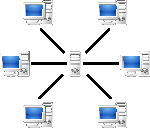
\includegraphics[width=\linewidth]{./Images/Chapter09/figIX-02a-server-based-network.pdf}
\caption{\label{fig:IX.1a}Réseau « client-serveur ».}
\end{subfigure}\\[6pt]
\begin{subfigure}{\linewidth}
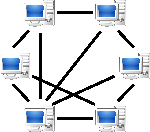
\includegraphics[width=\linewidth]{./Images/Chapter09/figIX-02b-p2p-network.pdf}
\caption{\label{fig:IX.1b}Réseau « pair-à-pair ».}
\end{subfigure}
}

%--- BUG: NO AUTOMATIC DETECTION BUT IT WORKS WITH \sidefigure!!! WHY???
%\begin{marginfigure}
%\begin{subfigure}{\linewidth}
%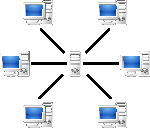
\includegraphics[width=\linewidth]{./Images/Chapter09/figIX-02a-server-based-network.pdf}
%\caption{\label{fig:IX.1a}Réseau « client-serveur ».}
%\end{subfigure}\\[6pt]
%\begin{subfigure}{\linewidth}
%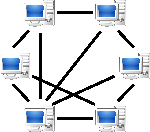
\includegraphics[width=\linewidth]{./Images/Chapter09/figIX-02b-p2p-network.pdf}
%\caption{\label{fig:IX.1b}Réseau « pair-à-pair ».}
%\end{subfigure}
%\caption{\label{fig:IX.1}Typologie des réseaux.}
%\end{marginfigure}


\overparagraph{Ce que dit le programme}

%\pagebreak

\begin{tcolorbox}[title={Protocole TCP/IP}, toprule=0pt, leftrule=0pt, rightrule=0pt, arc=0pt,
                  fonttitle=\scshape\boxtitlefont,
                  colbacktitle=white, coltitle=firstcolor, colframe=firstcolor, colback=firstcolor!10,
                  breakable, enhanced jigsaw]
Internet est défini par le protocole IP (\textit{Internet Protocol}), ensemble de normes qui permettent d’identifier et de nommer de façon uniforme tous les ordinateurs ou objets qui lui sont connectés. IP est accompagné de protocoles de transmission pour transférer l’information par \emph{paquets}, le principal étant TCP/IP (\textit{Transmission Control Protocol}). De nature logicielle, Internet s’appuie sur une grande variété de réseaux physiques où IP est implémenté. Il uniformise l’accès à tous les ordinateurs, les téléphones et les objets connectés.
\end{tcolorbox}

\begin{tcolorbox}[title={Données et information}, toprule=0pt, leftrule=0pt, rightrule=0pt, arc=0pt,
                  fonttitle=\scshape\boxtitlefont,
                  colbacktitle=white, coltitle=firstcolor, colframe=firstcolor, colback=firstcolor!10,
                  breakable, enhanced jigsaw]
Internet manipule deux types d’information : les contenus envoyés et les adresses du destinataire et de l’émetteur. Ces deux types d’information sont regroupés dans des paquets de taille fixe, de façon uniforme et indépendante du type de données transportées : texte, images, sons, vidéos, etc. Les adresses sont numériques et hiérarchiques, comme \texttt{78.109.84.114}, mais l’utilisateur connaît surtout des adresses symboliques normalisées, comme \url{wikipedia.fr}. Le système DNS (\textit{Domain Name System}) transforme une adresse symbolique en adresse numérique. Il est réalisé par un grand nombre d’ordinateurs répartis sur le réseau et constamment mis à jour.
\end{tcolorbox}

\begin{tcolorbox}[title={Algorithmes et programmes}, toprule=0pt, leftrule=0pt, rightrule=0pt, arc=0pt,
                  fonttitle=\scshape\boxtitlefont,
                  colbacktitle=white, coltitle=firstcolor, colframe=firstcolor, colback=firstcolor!10,
                  breakable, enhanced jigsaw]
Lors du routage, un paquet peut ne pas arriver pour deux raisons : une panne matérielle d’une ligne ou d’un routeur, ou sa destruction. Chaque paquet contient l’information d’un nombre maximal de routeurs à traverser : pour ne pas encombrer le réseau, il est détruit si ce nombre est atteint. C’est le protocole TCP qui fiabilise la communication en redemandant les paquets manquants. Il garantit que tout paquet finira par arriver, sauf panne matérielle incontournable. TCP réordonne aussi les paquets arrivés dans le désordre et diminue la congestion du réseau en gérant au mieux les redemandes. Mais ni Internet ni TCP ne possèdent de garantie temporelle d’arrivée des paquets, ce qui nuit à la qualité de la diffusion du son ou des vidéos et de la téléconférence. En effet, dans une vidéo on peut perdre une image isolée, mais pas le fil du temps.

D’autres protocoles s’appuient sur ceux d’Internet, par exemple les protocoles du Web (HTTP et HTTPS) et le protocole NTP (\textit{Network Time Protocol}) qui permet de synchroniser finement les heures des ordinateurs et objets connectés.
\end{tcolorbox}

\begin{jazzfigure*}
\Centering
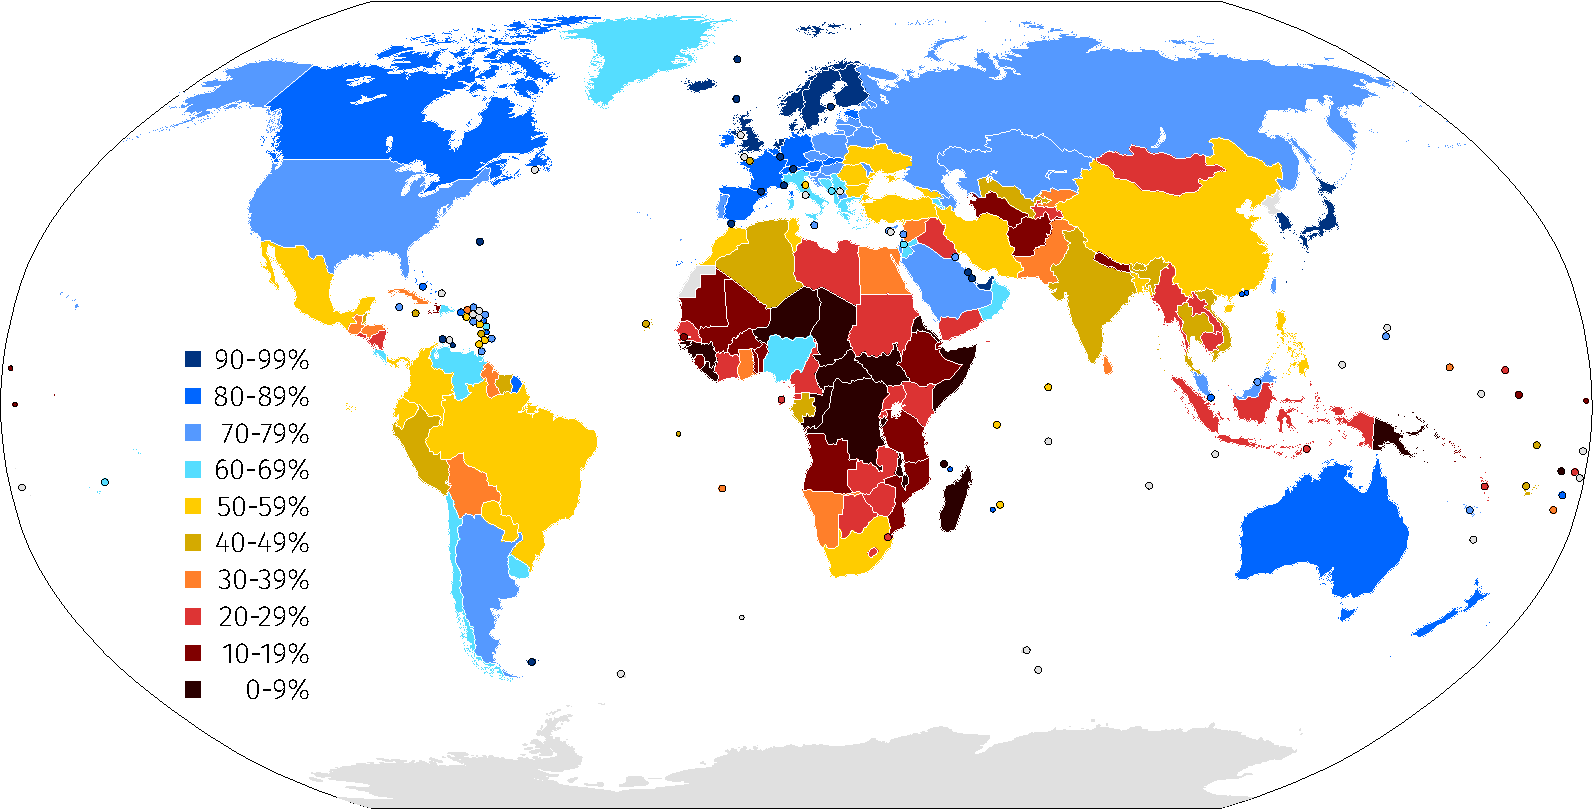
\includegraphics[width=\linewidth]{./Images/Chapter09/figIX-01-internet-penetration-map-2016-update.pdf}
\caption{\label{fig:IX.2}Taux de pénétration de l'Internet par pays (mise à jour 2016).}
\end{jazzfigure*}
\vspace*{-16pt}


\begin{tcolorbox}[title={Machines}, toprule=0pt, leftrule=0pt, rightrule=0pt, arc=0pt,
                  fonttitle=\scshape\boxtitlefont,
                  colbacktitle=white, coltitle=firstcolor, colframe=firstcolor, colback=firstcolor!10,
                  breakable, enhanced jigsaw]
Réseau mondial, Internet fonctionne au moyen de routeurs, de lignes de transmissions à très hauts débits (fibres optiques) entre routeurs, de réseaux de téléphonie mobile, et de réseaux locaux. Ses protocoles étant logiciels, il peut s’appuyer \emph{sur n’importe quel réseau physique} qui les implémente : 4G, Ethernet, ADSL, Wi-Fi, Bluetooth, etc. TCP/IP n’est pas implémenté dans l’infrastructure, mais dans chacun des ordinateurs connectés et un serveur DNS est aussi un ordinateur connecté. Des mécanismes complexes assurent la continuité de la connexion, par exemple pour passer sans interruption de téléphonie 4G au Wi-Fi ou son ubiquité, par exemple pour passer de façon invisible d’antenne à antenne avec un téléphone portable quand on voyage.

Dans les \emph{réseaux pair-à-pair} s’appuyant sur Internet et souvent utilisé pour le transport de vidéos, chaque ordinateur sert à la fois d’émetteur et de récepteur.
\end{tcolorbox}

\overparagraph{Web-conférence}

\begin{marginvideo}
	[\label{vid:IX.3}Internet et les réseaux, Benoît \textsc{Parrein}.]%
	\movie[width=\marginparwidth,showcontrols]%
		{
\includegraphics[width=\marginparwidth]{./Images/Pictograms/film-strip-dark-electric-blue.png}}%
		{./Videos/Chapter09/vidIX-03-conf-snt-internet-benoit-parrein.mp4}%
	\launchvideo{./Videos/Chapter09/vidIX-03-conf-snt-internet-benoit-parrein.mp4}
\end{marginvideo}

\textsc{Class'Code} \textsc{Pays-de-Loire} a organisé des conférences qui abordent les sept thématiques du programme SNT. Leur objectif est de fournir une vue d’ensemble et de poser les bases nécessaires à l’appropriation de ces grands domaines sous deux angles définis par le programme :
\begin{itemize}
\item une présentation historique (30 à 45 minutes) : grandes étapes de création/développement, acteurs majeurs, contexte général, histoire des idées et mise en contexte suffisamment fiable pour être réutilisée en cours ;
\item des exemples concrets de ce qui est étudié ou produit dans ces domaines et une réflexion sur les besoins et enjeux actuels et à venir à travers un débat (45 à 60 minutes) qui laisse la parole à des personnes travaillant dans ces champs de spécialité  (chercheurs, enseignants, étudiants, entreprises...), que ce soit en recherche ou en entreprise.
\end{itemize}

La conférence sur la thématique Internet a eu lieu le 12 mars 2019 dans le cadre du projet \textsc{Class'Code} à l’Université de Nantes. Elle a été retransmise en ligne et est maintenant disponible sur \textsc{YouTube}.

\begin{gofurther}{Ressources complémentaires}
\lightbf{Se former}
\begin{itemize}\jazzitem
\item La Partie 2 de la \href{https://pixees.fr/classcode/formations/module4/\#partie2}{formation \textsc{Class´Code} sur les réseaux} permet de \href{https://openclassrooms.com/fr/courses/4297411-connecter-le-reseau/4304576-decouvrez-comment-l-information-circule-sur-le-reseau}{comprendre comment l’information circule} sur le réseau, et de \href{https://openclassrooms.com/fr/courses/4297411-connecter-le-reseau/4304581-partez-a-la-decouverte-des-acteurs-du-net}{découvrir les acteurs du Net}.
\item La Partie 3 de la \href{https://pixees.fr/classcode/formations/module4/\#partie3}{formation \textsc{Class´Code} sur les réseaux} permet de \href{https://openclassrooms.com/fr/courses/4297411-connecter-le-reseau/4304631-mais-qu-est-ce-qu-un-protocole}{comprendre ce qu'est un protocole} et d'appréhender l'\href{https://openclassrooms.com/fr/courses/4297411-connecter-le-reseau}{évolution des réseaux}.
\item Pour les enseignants : la \href{https://magistere.education.fr/dgesco/}{conférence de Christine \textsc{Gaubert-Macon} sur le Web, Internet et les réseaux sociaux}, lors des formations nationales, accès par m@gistere (réservé aux enseignant·e·s).
\item Une \href{https://interstices.info/dossier/snt-internet/}{sélection d'articles} du site \textsc{Interstices}.
\end{itemize}

\vspace{2pt}
\lightbf{Ouvrages}
\begin{itemize}\jazzitem
\item Fabien \textsc{Tarissan} (2019) « Au cœur des réseaux : des sciences aux citoyens », Édition le Pommier. Il traite de science, plus particulièrement des réseaux (informatiques et autres), des algorithmes qui y opèrent et de l'impact qu'ils ont sur notre manière de nous informer en ligne (\textit{fake news}, publicité ciblée, données personnelles, etc.), et de l'économie sous-jacente.
\item Valérie \textsc{Schafer} (2018) « En construction : La fabrique française d'Internet et du Web dans les années 1990 », INA.
\item Stéphane \textsc{Bortzmeyer} (2018) « Cyberstructure : L'Internet, un espace politique », C{\&}F Édition.
\end{itemize}

\vspace{2pt}
\lightbf{Créer son cours}
\begin{itemize}\jazzitem
\item La \href{https://www.isoloir.net/}{ressource « isoloir »} propose une activité sur la régulation d'Internet, ces \href{https://pixees.fr/informatique-et-societe-du-jeu-serieux-au-document-pedagogique/}{documents} sont librement réutilisables.
\item Comment \href{http://www.adjectif.net/spip/spip.php?article294}{relier la notion d'URL avec les couches réseaux d'Internet}.
\item Une \href{https://www.isoloir.net/documents01/videos/ISOLOIR_CN_ALL_Trala01_ok_Bases.mp4}{vidéo explicative d'Internet} pour les lycéen·ne·s.
\item Le \href{https://pixees.fr/le-numerique-la-loi-et-notre-vie-privee-2/}{numérique, la loi et notre vie privée}.
\end{itemize}
\end{gofurther}


\subsection[Réaliser des activités]{Réaliser des activités}
\label{sub:IX.1.2}

\overparagraph*{Exemple d'activités}

Les activités proposées\caution[t]<firstcolor>{%
Toutes les fiches actuellement collectées sont disponibles à l'URL : \url{http://tinyurl.com/yx9qce8s} et on peut aussi proposer des activités.}{Note de la rédaction}
sont disponibles sous forme de fiches à télécharger (format ODT de la suite bureautique libre \textsc{LibreOffice}).

\begin{jazzitemize}
\item \textdoc{./Documents/Chapter09/cardIX-01-snt-internet-david-roche.odt}{Introduction à Internet : réseau de réseaux, adresse IP}.
\item \textdoc{./Documents/Chapter09/cardIX-02-snt-tcp-ip-david-roche.odt}{Notion de protocole, TCP/IP, encapsulation des données}.
\item \textdoc{./Documents/Chapter09/cardIX-03-snt-routing-david-roche.odt}{Notion de routage des paquets}.
\item \textdoc{./Documents/Chapter09/cardIX-04-snt-net-simulation-david-roche.odt}{Prise en main du logiciel de simulation réseau Filius}.
\item \textdoc{./Documents/Chapter09/cardIX-05-snt-dns-david-roche.odt}{Introduction à la notion de DNS (\textit{Domain Name Server})}.
\item \textdoc{./Documents/Chapter09/cardIX-06-snt-p2p-david-roche.odtacti}{Introduction aux réseaux pair-à-pair}.
\item \textdoc{./Documents/Chapter09/}{Activité déconnectée/connectée, routage entre routeurs}.
\end{jazzitemize}

\noindent Fiche d'activité élève :
\begin{jazzitemize}
\item \pdfdoc{./Documents/Chapter09/activityIX-01-snt-ethernet-lan.pdf}{Observer une communication en réseau Ethernet}.
\end{jazzitemize}

%\overparagraph{Ce que propose le programme}

\begin{tcolorbox}[title={Ce que propose le programme}, toprule=0pt, leftrule=0pt, rightrule=0pt, arc=0pt,
                  fonttitle=\scshape\boxtitlefont,
                  colbacktitle=white, coltitle=firstcolor, colframe=firstcolor, colback=firstcolor!10,
                  breakable, enhanced jigsaw]
\begin{jazzitemize}
\item Illustrer le fonctionnement du routage et de TCP par des activités  débranchées ou à l’aide de logiciels dédiés, en tenant compte de la destruction de paquets.   
\item Déterminer l’adresse IP d’un équipement et l’adresse du DNS sur un réseau. 
\item Analyser son réseau local pour observer ce qui y est connecté. 
\item Suivre le chemin d’un courriel en utilisant une commande du protocole IP. 
\end{jazzitemize}
\end{tcolorbox}

\begin{jazztable*}
\caption{\label{tab:IX.1}Internet : compétences attendues chez les élèves.}
\Centering
\begingroup
\small
\renewcommand*{\arraystretch}{1.6}
\rowcolors{2}{tableLineOne}{tableLineTwo}
\begin{tabularx}{\linewidth}{lX}
\rowcolor{secondcolor}
\multicolumn{2}{c}{\Gape[6pt]{\textcolor{white}{\textbf{Internet}}}} \\
\rowcolor{firstcolor}
\multicolumn{1}{c}{\scshape\titlingfont\textcolor{white}{Contenus}} 
	&	\multicolumn{1}{c}{\scshape\titlingfont\textcolor{white}{Capacités attendues}} \\
Protocole  TCP/IP : paquets, routage des paquets
  & Distinguer le rôle des protocoles IP et TCP.\newline
    Caractériser les principes du routage et ses limites.\newline
    Distinguer la fiabilité de transmission\newline et l’absence de garantie temporelle. \\
Adresses symboliques et serveurs DNS 
  & Sur des exemples réels, retrouver une adresse IP\newline à partir d’une adresse symbolique et inversement.\\
Réseaux pair-à-pair &
  Décrire l’intérêt des réseaux pair-à-pair\newline ainsi que les usages illicites qu’on peut en faire.\\
Indépendance d’Internet par rapport au réseau physique &
  Caractériser quelques types de réseaux physiques :\newline obsolètes ou actuels, rapides ou lents, filaires ou non.\newline
  Caractériser l’ordre de grandeur du trafic de données\newline sur internet et son évolution.
\end{tabularx}%
\endgroup
\end{jazztable*}



%----------
\section[Web et information]{Web et information}
\label{sec:IX.2}

\subsection[Découvrir la thématique]{Découvrir la thématique}
\label{sub:IX.2.1}

\subsubsection[Ancrage dans le réel]{Ancrage dans le réel}
\label{subsub:IX.2.1.1}

\overparagraph{Points-clés}

\begin{marginvideo}
	[\label{vid:IX.4}Web et information.]%
	\movie[width=\marginparwidth,showcontrols]%
		{
\includegraphics[width=\marginparwidth]{./Images/Pictograms/film-strip-dark-electric-blue.png}}%
		{./Videos/Chapter09/vidIX-04-mooc-snt-web.mp4}%
	\launchvideo{./Videos/Chapter09/vidIX-04-mooc-snt-web.mp4}
\end{marginvideo}

\begin{jazzitemize}
\item Le Web est à la fois un \emph{espace documentaire} dans lequel on trouve de l'information (Web 1.0), un \emph{espace social et participatif} dans lequel on crée soi-même de l'information pour la partager (Web 2.0),  et un \emph{espace applicatif} dans lequel on interagit avec des logiciels qui offrent un certain nombre de fonctionnalités.
\item Le \emph{Web dit sémantique} (Web 3.0) est un \emph{espace où la connaissance est structurée} de manière à être manipulée par des algorithmes qui interagissent à travers le Web pour proposer des services et un espace (Web 4.0) dans lequel les \emph{objets connectés} eux-mêmes peuvent interagir entre eux.
\item Cette révolution génère de \emph{nouveaux métiers} et de \emph{nouvelles façons de travailler}, et conduit à la \emph{dématérialisation} des services (administratifs, etc…). Contrairement à une idée reçue \href{https://fr.wikipedia.org/wiki/D\%C3\%A9mat\%C3\%A9rialisation\#Aspects_environnementaux}{elle génère plus qu'elle ne réduit} les impacts environnementaux.
\item \href{https://fr.wikipedia.org/wiki/Tim_Berners-Lee}{Tim Berners-Lee} disait récemment que le Web, « \textit{conçu comme un outil ouvert, collaboratif et émancipateur, a été détourné par des escrocs et des \textup{trolls}, qui l’ont utilisé pour manipuler le reste des internautes à travers le monde} » et « \textit{il n'est pas trop tard pour changer le Web} » conclut-il positivement.
\item Il faut aussi comprendre le Web non référencé, \href{https://fr.wikipedia.org/wiki/Web_profond}{Web profond} à également distinguer du \href{https://fr.wikipedia.org/wiki/Dark_web}{\textit{Dark Web}}. Ce dernier, sans fantasmer, est un phénomène important de société en lien avec une réalité socio-économi\-que à connaître.
\end{jazzitemize}

%\sidegraphic{
\includegraphics[width=\linewidth]{./Images/Chapter09/wikipedia-logo-v2-fr.pdf}}{Wikimedia Foundation}%
\begin{margingraphic}{-20pt}

\includegraphics[width=\linewidth]{./Images/Chapter09/wikipedia-logo-v2-fr.pdf}
\end{margingraphic}


\overparagraph{Mots-clés}

\begin{jazzitemize}
\item Le \href{https://fr.wikipedia.org/wiki/World_Wide_Web}{Web}, une des applications d'\href{https://fr.wikipedia.org/wiki/Internet}{Internet},
\item L'encyclopédie \href{https://fr.wikipedia.org/wiki/Wikip\%C3\%A9dia}{Wikipédia}.
\item La \href{https://fr.wikipedia.org/wiki/D\%C3\%A9mat\%C3\%A9rialisation}{dématérialisation} d'une organisation.
\end{jazzitemize}

\overparagraph{Ce que dit le programme}

\begin{tcolorbox}[title={Introduction}, toprule=0pt, leftrule=0pt, rightrule=0pt, arc=0pt, fonttitle=\scshape\boxtitlefont,
                  colbacktitle=white, coltitle=firstcolor, colframe=firstcolor, colback=firstcolor!10,
                  breakable, enhanced jigsaw]
Le Web (toile ou réseau) désigne un système donnant accès à un ensemble de données (page, image, son, vidéo) reliées par des liens hypertextes et accessibles sur le réseau Internet.
\end{tcolorbox}

\begin{jazzgraphic*}
%\begin{tikzpicture}[remember picture, overlay]
%\node[anchor=east, inner sep=0pt, rotate=-90, xshift=0pt, yshift=(\linewidth+6pt)] 
%	at (0,0) {\scriptsize\faCopyright\space Gerd Altmann \textit{via} \href{https://pixabay.com}{Pixabay}};
%\end{tikzpicture}%
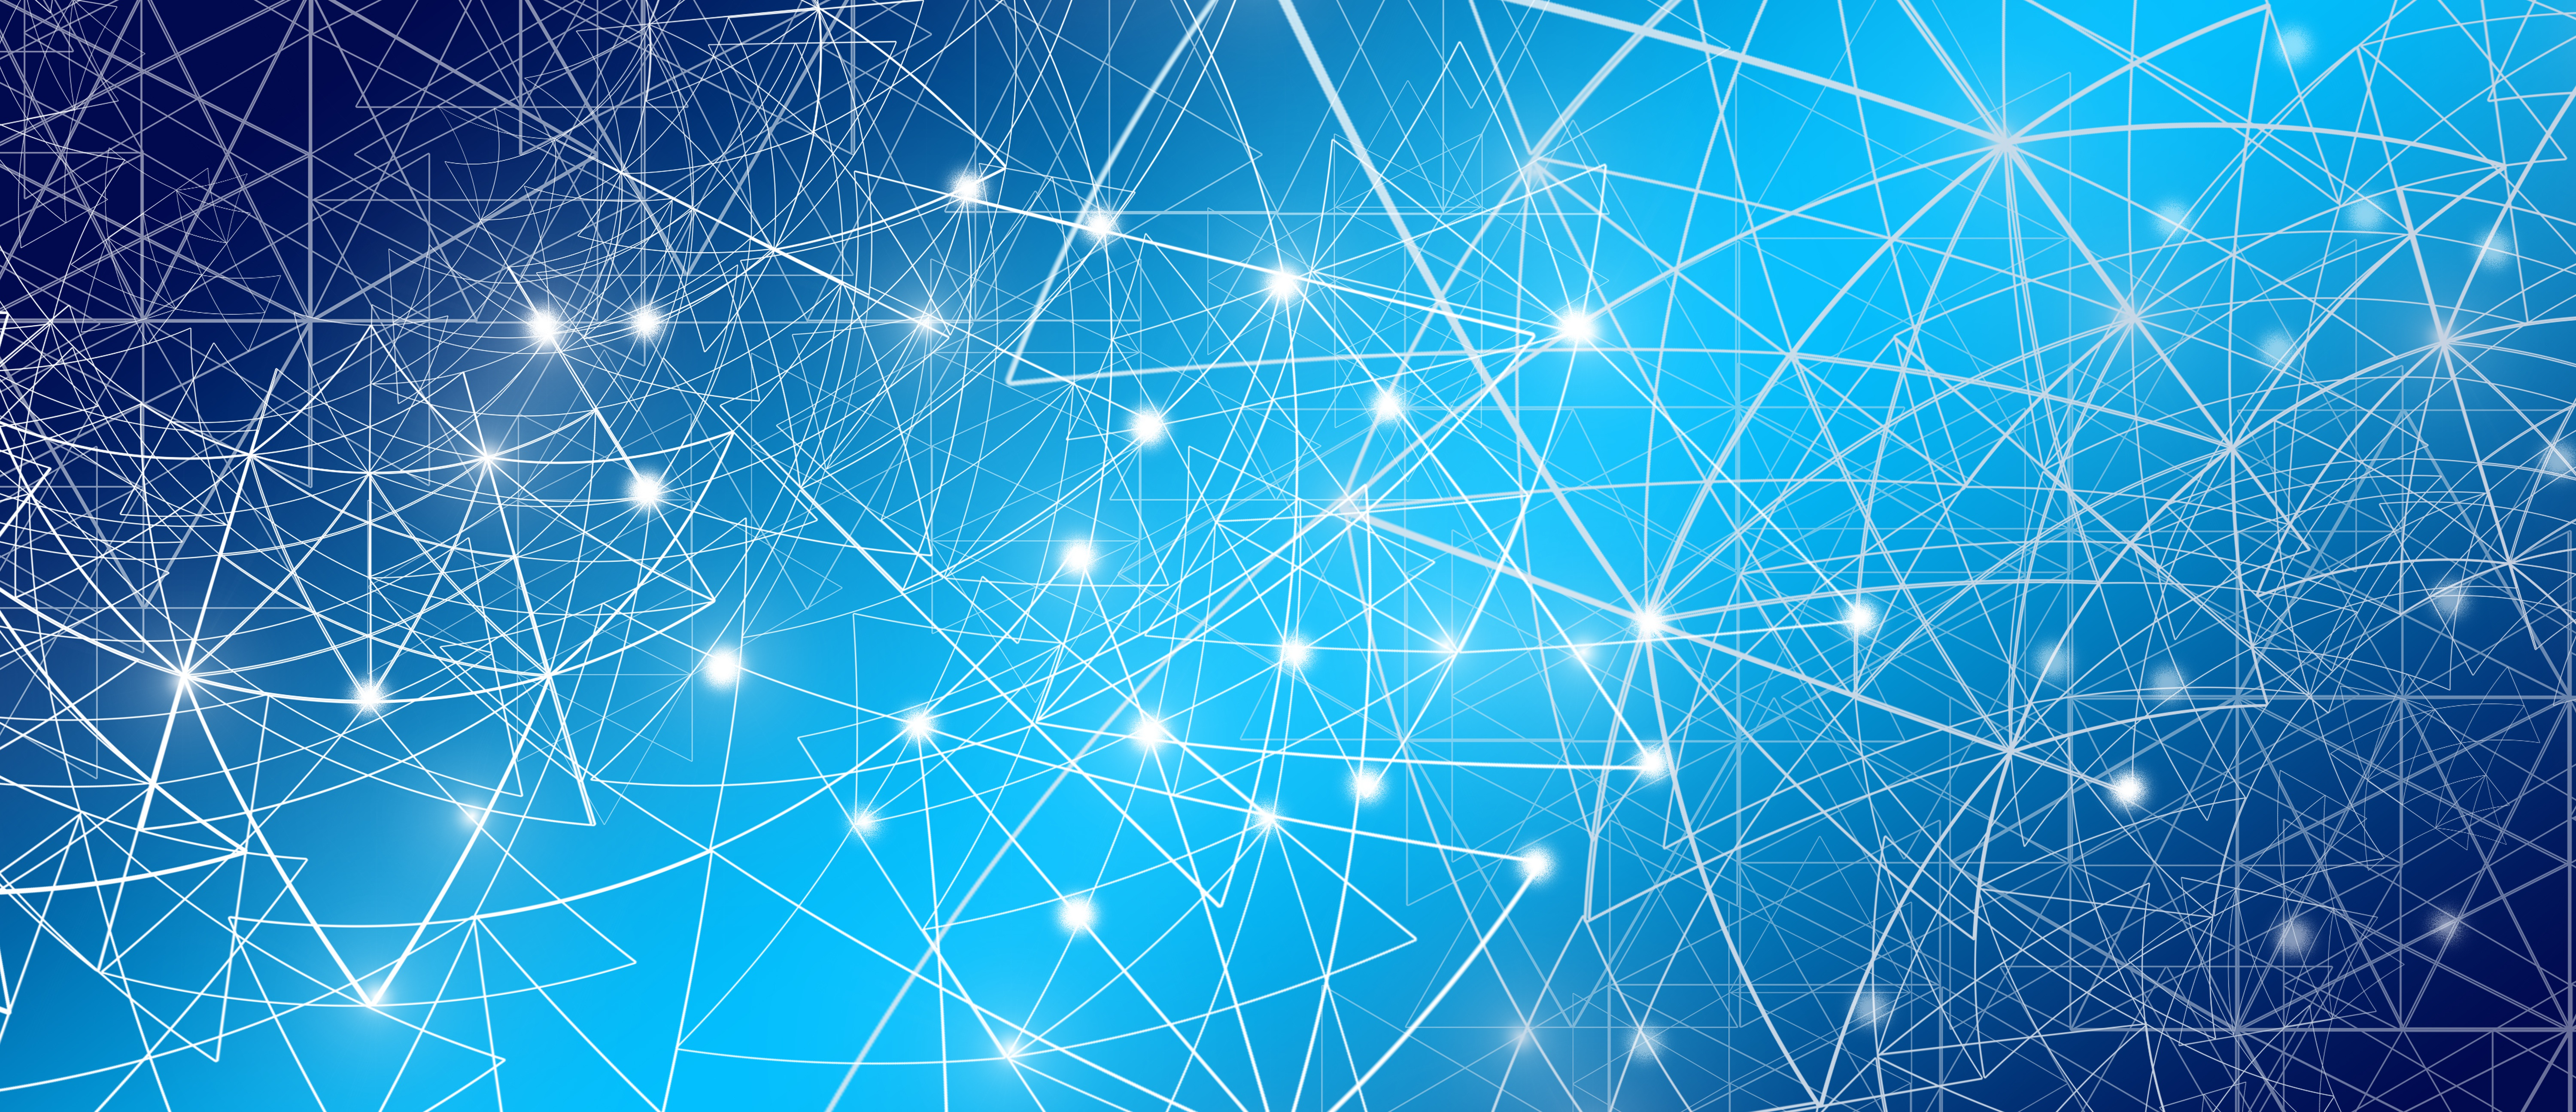
\includegraphics[width=\linewidth]{./Images/Chapter09/network-gerd-altmann-pixabay.jpg}%
\begin{tikzpicture}[remember picture, overlay]
\node[anchor=west, inner sep=0pt, rotate=90, xshift=0pt, yshift=(\linewidth+6pt)] 
	at (0,0) {\scriptsize\faCopyright\space Gerd Altmann \textit{via} \href{https://pixabay.com}{Pixabay}};
\end{tikzpicture}%
\end{jazzgraphic*}

\begin{tcolorbox}[title={Impacts sur les pratiques humaines}, toprule=0pt, leftrule=0pt, rightrule=0pt, arc=0pt,
                  fonttitle=\scshape\boxtitlefont,
                  colbacktitle=white, coltitle=firstcolor, colframe=firstcolor, colback=firstcolor!10,
                  breakable, enhanced jigsaw]
Dans l’histoire de la communication, le Web est une révolution : il a ouvert à tous la possibilité et le droit de publier ; il permet une coopération d’une nature nouvelle entre individus et entre organisations : commerce en ligne, création et distribution de logiciels libres multi-auteurs, création d’encyclopédies mises à jour en permanence, etc. ; il devient universel pour communiquer avec les objets connectés.

Le Web permet aussi de diffuser toutes sortes d’informations dont ni la qualité, ni la pertinence, ni la véracité ne sont garanties et dont la vérification des sources n’est pas toujours facile. Il conserve des informations, parfois personnelles, accessibles partout sur de longues durées sans qu’il soit facile de les effacer, ce qui pose la question du droit à l’oubli. Il permet une exploitation de ses données, dont les conséquences sociétales sont encore difficiles à estimer : recommandation à des fins commerciales, bulles informationnelles, etc. En particulier, des moteurs de recherche permettent à certains sites d’acquérir de la visibilité sur la première page des résultats de recherche en achetant de la publicité qui apparaîtra parmi les liens promotionnels. 
\end{tcolorbox}

\subsubsection[Volet historique]{Volet historique}
\label{subsub:IX.2.1.2}

\begin{marginvideo}
	[\label{vid:IX.5}Naissance du Web.]%
	\movie[width=\marginparwidth,showcontrols]%
		{
\includegraphics[width=\marginparwidth]{./Images/Pictograms/film-strip-dark-electric-blue.png}}%
		{./Videos/Chapter09/vidIX-05-mooc-snt-naissance-web.mp4}%
	\launchvideo{./Videos/Chapter09/vidIX-05-mooc-snt-naissance-web.mp4}
\end{marginvideo}

C’est en 1990 que Tim \textsc{Berners-Lee} et Robert \textsc{Cailliau}, chercheurs au \textsc{Cern} (Organisation européenne pour la recherche nucléaire), conçoi\-vent le premier site Internet en HTML (langage informatique utilisé pour développer les sites Web) et inventent le protocole HTTP. En bref, le Web est issu d’un croisement d’idées qui ont bien progressé depuis sa création : pour que le Web reste un lieu libre et ouvert, nous devons nous l'approprier !

Consulter la vidéo \cref{vid:IX.5} et le \href{https://openclassrooms.com/fr/courses/4297411-connecter-le-reseau/4304506-assistez-a-la-naissance-du-web#r-4344123}{chapitre sur le Web d'OpenClassrooms} pour disposer d'un historique du Web. 


\noindent Source : module 4, \href{https://pixees.fr/classcode/formations/module4/}{formation Class'Code}.

\overparagraph*{Ce que dit le programme}


\begin{tcolorbox}[title={Repères historiques}, toprule=0pt, leftrule=0pt, rightrule=0pt, arc=0pt,
                  fonttitle=\scshape\boxtitlefont,
                  colbacktitle=white, coltitle=firstcolor, colframe=firstcolor, colback=firstcolor!10,
                  breakable, enhanced jigsaw]
\begin{jazzitemize}
\item 1965 : invention du concept d’hypertexte par Ted \textsc{Nelson}.
\item 1989 : naissance au CERN par Tim \textsc{Berners-Lee}.
\item 1993 : mise dans le domaine public, disponibilité du premier navigateur Mosaic.
\item 1995 : mise à disposition de technologies pour le développement de site Web interactif (JavaScript) et dynamique (PHP).
\item 2001 : pages standardisées grâce au \textit{Document Object Model}.
\item 2010 : mise à disposition de technologies pour le développement  d’applications sur mobiles.
\end{jazzitemize}
\end{tcolorbox}

\subsubsection[Explication des notions]{Explication des notions}
\label{subsub:IX.2.1.3}

\overparagraph{Idées-forces}

\begin{margingraphic}
\Centering

\includegraphics[width=.75\linewidth]{./Images/Chapter09/html5-logo.pdf}\\

\includegraphics[width=.75\linewidth]{./Images/Chapter09/css-logo.pdf}\\

\includegraphics[width=.75\linewidth]{./Images/Chapter09/javascript-logo.pdf}
\end{margingraphic}

\begin{jazzitemize}
\item Le langage HTML5  permet de définir une page Web, ses métadonnées qui sont dans l'entête (balise \texttt{<head>}) et son contenu dans le corps de la page (balise \texttt{<body>}),  la mise en page est elle déléguée aux directives du CSS.
\item Dans une page Web on peut mettre des éléments d'interaction, par exemple des champs de formulaire ou des éléments cliquables, du code JavaScript va alors permettre de rendre ces éléments actifs.
\item Les adresses internet, ou URL (Localisation de Ressources Universelles), constituent un petit langage qui permet de localiser un conte\-nu,  mais aussi de faire une requête sur ce contenu.  Chaque partie de l'URL correspond à un paramètre.
\item Le protocole HTTP  permet de faire une requête Web et d'obtenir la réponse, c'est le mécanisme standard qui permet d'utiliser le Web.
\end{jazzitemize}

\overparagraph{Mots-clefs}

\begin{jazzitemize}
\item Trois langages principaux des pages Web : \href{https://fr.wikipedia.org/wiki/HTML5}{HTML5}, \href{https://fr.wikipedia.org/wiki/Feuilles_de_style_en_cascade\#CSS3}{CSS3}, \href{https://fr.wikipedia.org/wiki/JavaScript}{JavaScript}.
\item Protocole \href{https://fr.wikipedia.org/wiki/Hypertext_Transfer_Protocol}{HTTP} du Web et sa variante sécurisée \href{https://fr.wikipedia.org/wiki/HyperText_Transfer_Protocol_Secure}{HTTPS}.
\item Notion de \href{https://fr.wikipedia.org/wiki/Moteur_de_recherche}{moteur de recherche}.
\item Environnement \href{https://fr.wikipedia.org/wiki/Client-serveur}{client-serveur}.
\end{jazzitemize}

\overparagraph{Ce que dit le programme}

\begin{tcolorbox}[title={Normalisation de la présentation}, toprule=0pt, leftrule=0pt, rightrule=0pt, arc=0pt,
                  fonttitle=\scshape\boxtitlefont,
                  colbacktitle=white, coltitle=firstcolor, colframe=firstcolor, colback=firstcolor!10,
                  breakable, enhanced jigsaw]
Sur le Web, les textes, photos, vidéos, graphiques, sons, programmes sont exprimés et assemblés dans divers formats normalisés par un consortium mondial (W3C : \textit{World Wide Web Consortium}), ce qui permet une circulation standardisée de toutes ces informations.

Les pages Web sont écrites dans le langage de balises HTML (Hypertext Markup Language). Leur style graphique est défini dans le langage CSS (\textit{Cascading Style Sheets}).

Les pages ont une adresse unique, nommée URL (\textit{Uniform Ressource Locator}). Elles sont accessibles \textit{via} Internet en utilisant le protocole HTTP (Hypertext Transfer Protocol) ou sa version sécurisée HTTPS qui crypte les échanges. L’affichage des pages est réalisé chez l’utilisateur par un programme appelé navigateur.

Un hypertexte est un texte augmenté de renvois automatiques à des textes, des images ou des sons. Initialement, un hypertexte se restreignait à la mémoire d’un seul ordinateur. Dans une page Web, ce renvoi se fait sur n’importe quelle machine du réseau internet, par le truchement de l’adresse de la page Web du texte (URL) auquel il fait référence. La toile d’araignée construite par les liens peut être représentée sous forme d’un graphe qui matérialise la structure du Web.
\end{tcolorbox}

\begin{jazzgraphic*}
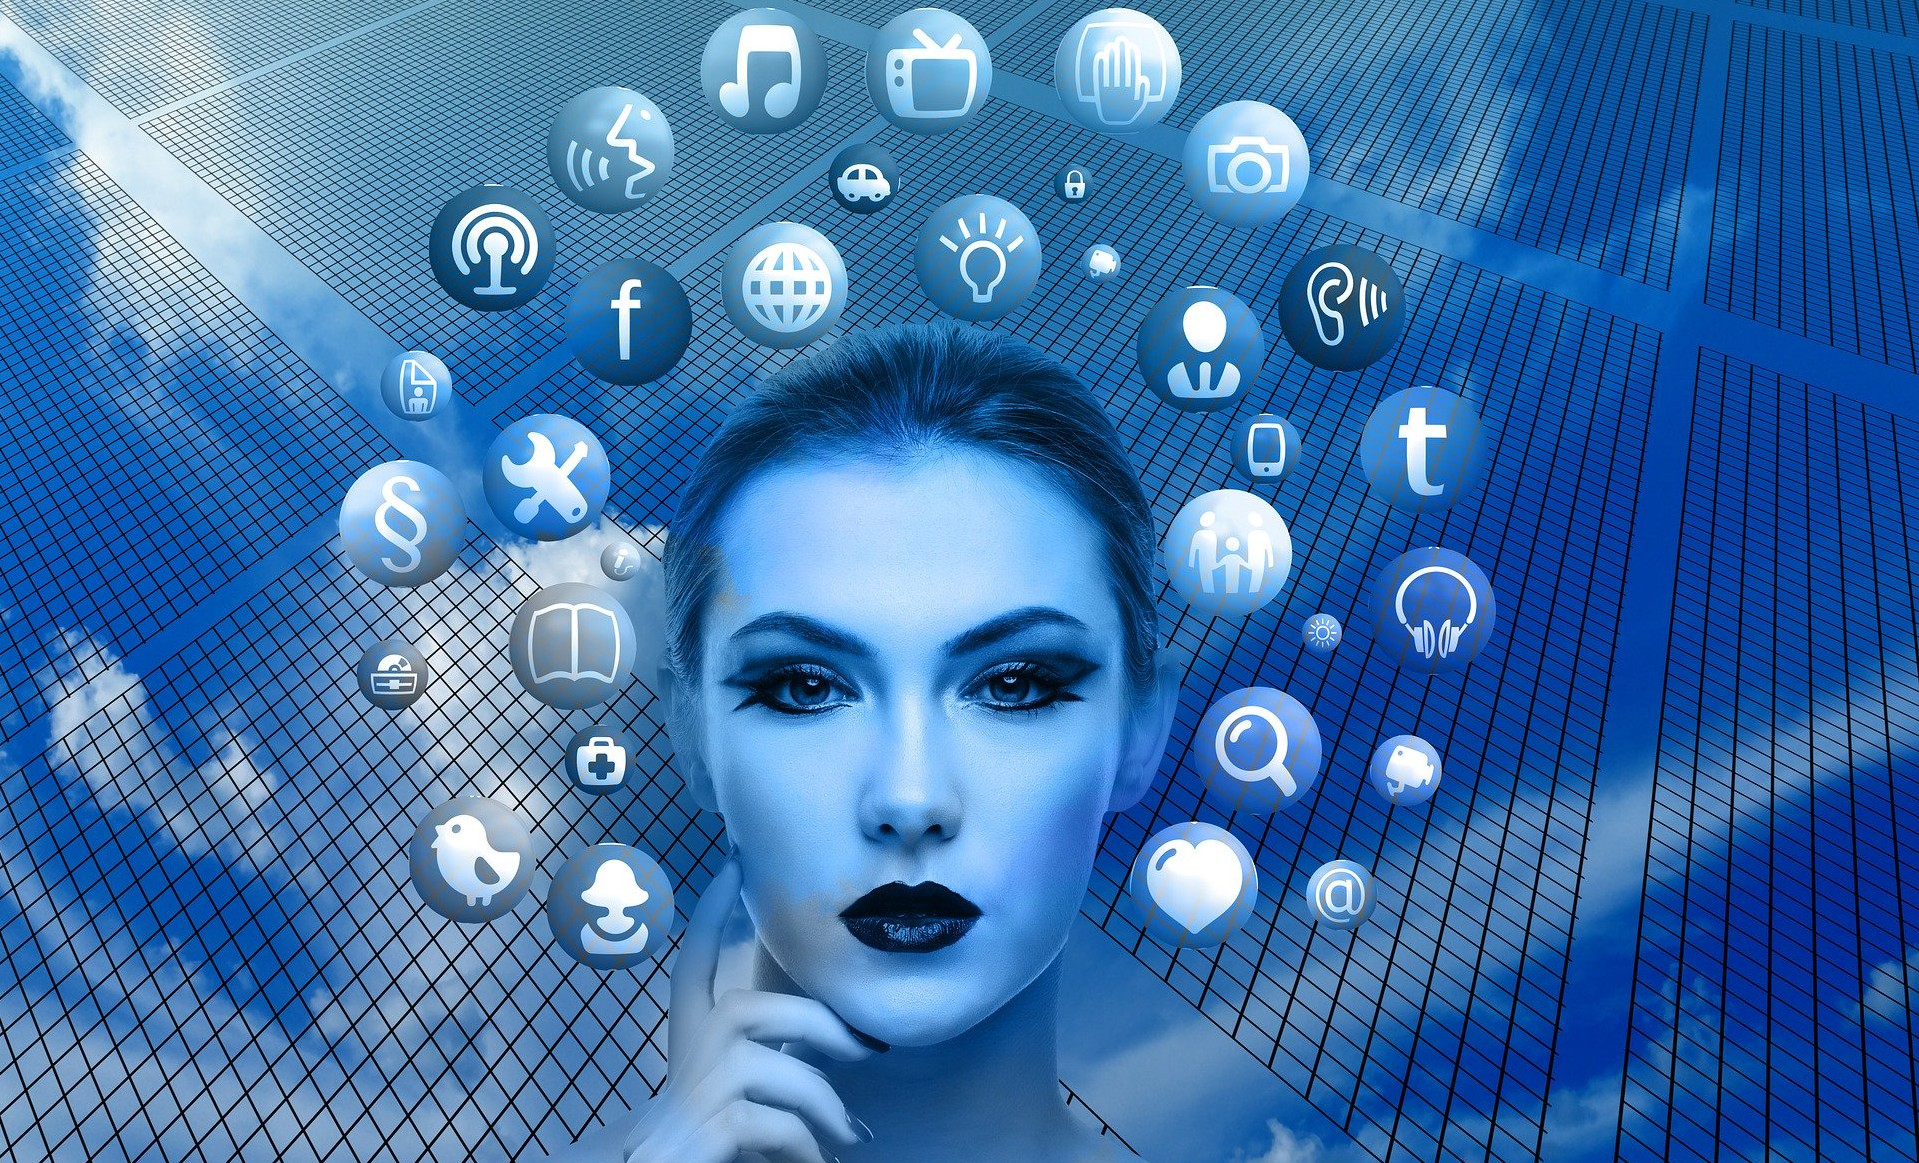
\includegraphics[width=\linewidth]{./Images/Chapter09/woman-applications-gerd-altmann-pixabay.jpg}%
\begin{tikzpicture}[remember picture, overlay]
\node[anchor=west, inner sep=0pt, rotate=90, xshift=0pt, yshift=(\linewidth+6pt)] 
	at (0,0) {\scriptsize\faCopyright\space Gerd Altmann \textit{via} \href{https://pixabay.com}{Pixabay}};
\end{tikzpicture}
\end{jazzgraphic*}

\begin{tcolorbox}[title={Moteurs de recherche}, toprule=0pt, leftrule=0pt, rightrule=0pt, arc=0pt,
                  fonttitle=\scshape\boxtitlefont,
                  colbacktitle=white, coltitle=firstcolor, colframe=firstcolor, colback=firstcolor!10,
                  breakable, enhanced jigsaw]
 Les moteurs de recherche permettent de trouver des informations dans des pages dont on ne connaît pas l’adresse, voire dont on ignore l’existence. La méthode de recherche appelée référencement naturel se décompose en trois grandes activités, réalisées par les moteurs de recherche : (1) le parcours automatique du Web pour collecter les pages visitées (aspiration des pages Web effectuée par des robots) ; (2) l’analyse du contenu des pages et leur indexation sur les mots qu’elles contiennent (constitution d’un annuaire inversé qui associe à chaque terme les URL des pages où il apparaît) ; (3) la troisième activité, réalisée à chaque fois qu’un internaute fait une requête, construit une liste ordonnée des pages (classement) comportant les mots clés de la requête. Leur ordre dépend notamment de leur popularité (principe des liens), de leur pertinence (aux mots de la requête), et de l’ordre des termes de la requête.

Les concepteurs de site Web peuvent améliorer le référencement de leurs pages en choisissant bien les mots et en les plaçant à des endroits stratégiques dans les pages.
\end{tcolorbox}

\begin{tcolorbox}[title={Interaction client/serveur}, toprule=0pt, leftrule=0pt, rightrule=0pt, arc=0pt,
                  fonttitle=\scshape\boxtitlefont,
                  colbacktitle=white, coltitle=firstcolor, colframe=firstcolor, colback=firstcolor!10,
                  breakable, enhanced jigsaw]
Le Web s’appuie sur le dialogue entre clients et serveurs. L’interaction est à l’initiative des clients (les applications qui se connectent au Web, dont les navigateurs), qui envoient des requêtes HTTP aux serveurs. Ces derniers renvoient leur résultat : des pages qu’ils ont stockées ou qu’ils créent dynamiquement en fonction de la requête formulée. Les pages reçues par les clients peuvent contenir des codes exécutables (souvent en JavaScript) qui permettent aux clients d’effectuer des traitements en accédant aux ressources de son ordinateur et en interagissant avec les serveurs.
Les applications peuvent être paramétrées pour autoriser ou interdire l’accès à des ressources locales aux programmes téléchargés par les pages.
\end{tcolorbox}


\begin{tcolorbox}[title={Sécurité et confidentialité}, toprule=0pt, leftrule=0pt, rightrule=0pt, arc=0pt,
                  fonttitle=\scshape\boxtitlefont,
                  colbacktitle=white, coltitle=firstcolor, colframe=firstcolor, colback=firstcolor!10,
                  breakable, enhanced jigsaw]
En formulant des requêtes sur des sites Web dynamiques et en laissant des programmes s’exécuter sur sa machine, l’utilisateur prend des risques : il peut communiquer des informations personnelles à son insu à des serveurs qui en gardent une trace, à distance ou localement par des \textit{cookies}, ou encore charger des pages contenant des programmes malveillants, par exemple permettant d’espionner en continu les actions de l’utilisateur. 

Par ailleurs, un navigateur peut garder un historique de toutes les interactions et le laisser accessible aux sites connectés. L’utilisateur peut utiliser des services qui s’engagent à ne pas garder de traces, comme certains moteurs de recherche. Il peut aussi \emph{paramétrer son navigateur} de façon à ce qu'il n’enregistre pas d’historique des interactions. De fausses pages peuvent encore être utilisées pour l’hameçonnage des utilisateurs. Un nom de lien pouvant cacher une adresse Web malveillante, il faut examiner cette adresse avant de l’activer par un clic.
\end{tcolorbox}

\overparagraph{Web-conférence}

\begin{marginvideo}
	[\label{vid:IX.6}Web et information, Julien \textsc{Pierre}.]%
	\movie[width=\marginparwidth,showcontrols]%
		{
\includegraphics[width=\marginparwidth]{./Images/Pictograms/film-strip-dark-electric-blue.png}}%
		{./Videos/Chapter09/vidIX-06-conf-snt-web-julien-pierre.mp4}%
	\launchvideo{./Videos/Chapter09/vidIX-06-conf-snt-web-julien-pierre.mp4}
\end{marginvideo}

\textsc{Class'Code} \textsc{Pays-de-Loire} a organisé des conférences qui abordent les sept thématiques du programme SNT. Leur objectif est de fournir une vue d’ensemble et de poser les bases nécessaires à l’appropriation de ces grands domaines sous deux angles définis par le programme :
\begin{itemize}
\item une présentation historique (30 à 45 minutes) : grandes étapes de création/développement, acteurs majeurs, contexte général, histoire des idées et mise en contexte suffisamment fiable pour être réutilisée en cours ;
\item des exemples concrets de ce qui est étudié ou produit dans ces domaines et une réflexion sur les besoins et enjeux actuels et à venir à travers un débat (45 à 60 minutes) qui laisse la parole à des personnes travaillant dans ces champs de spécialité  (chercheurs, enseignants, étudiants, entreprises...), que ce soit en recherche ou en entreprise.
\end{itemize}

La conférence sur \textit{Le Web et son information} a eu lieu le 26 mars 2019  dans le cadre du projet \textsc{Class'Code} à l’Université de Nantes. Elle a été retransmise en ligne et est maintenant disponible sur \textsc{YouTube}.

\begin{gofurther}{Ressources complémentaires}
\lightbf{Se former}
\begin{itemize}\jazzitem
\item La Partie 1 de la \href{https://pixees.fr/classcode/formations/module4/\#partie1}{formation \textsc{Class´Code} sur les réseaux} permet de se familiariser avec la création d'un site Web, au moyen d'un outil libre et facilement réutilisable.
\item La conférence de Fabien \textsc{Gandon} \href{http://www.mshsud.tv/spip.php?article632}{Les (r)évolutions de la planète Web}, 29 avril 2015.
\item Pour les enseignants : la \href{https://magistere.education.fr/dgesco/}{conférence de Christine \textsc{Gaubert-Macon} sur le Web, Internet et les réseaux sociaux}, lors des formations nationales, accès par m@gistere (réservé aux enseignant·e·s).
\item Le module 1 « Protéger ses données et son identité numérique~» et le module 4 « Navigation et traçage sur le Web » du \href{https://www.fun-mooc.fr/courses/course-v1:inria+41015+session03/about}{\textsc{Mooc} \textit{Protection de la vie privée dans le monde numérique}}, produit par l'\textsc{Inria} sur la plateforme FUN.
\item Une \href{https://interstices.info/dossier/snt-web/}{sélection d'articles} du site \textsc{Interstices}.
\end{itemize}

\vspace{2pt}
\lightbf{Créer son cours}
\begin{itemize}\jazzitem
\item Des animations intéressantes sur les réseaux sociaux et le web en général (les \textit{cookies}...) sur le site d'\href{https://donottrack-doc.com/fr/episodes/}{Arte}.
\item On dispose aussi sur \url{pixees.fr} d'une \href{https://pixees.fr/decouvrir-le-html/}{initiation à HTML} (avec une \href{https://pixees.fr/les-dessous-de-html-css-js-en-deux-idees-simples/}{présentation permettant de prendre du recul} et un \href{https://pixees.fr/quels-sont-les-droits-et-les-devoirs-des-webmestres/}{document sur les droits et devoirs à prendre en compte}).
\item \href{./Documents/Chapter09/memento_xhtml.pdf}{Memento HTML} et \href{./Documents/Chapter09/memento_css3.pdf}{memento CSS} pour les élèves.
\item \href{https://www.lemonde.fr/blog/binaire/2018/04/17/et-le-web-devint-semantique/}{\textit{Le Web devint sémantique}}, article de popularisation, revue en ligne \textsc{Binaire} sur le site du Monde, 17 avril 2018.
\end{itemize}
\end{gofurther}


\subsection[Réaliser des activités]{Réaliser des activités}
\label{sub:IX.2.2}

\overparagraph*{Exemple d'activités}

Les activités proposées\caution[t]<firstcolor>{%
Toutes les fiches actuellement collectées sont disponibles à l'URL : \url{http://tinyurl.com/yx9qce8s} et on peut aussi proposer des activités.}{Note de la rédaction}
sont disponibles sous forme de fiches à télécharger (format ODT de la suite bureautique libre \textsc{LibreOffice}).

\begin{jazzitemize}
\item \textdoc{./Documents/Chapter09/cardIX-08-snt-web-david-roche.odt}{Introduction à la notion de Web}.
\item \textdoc{./Documents/Chapter09/cardIX-09-snt-url-david-roche.odt}{Introduction à la notion d’URL}.
\item \textdoc{./Documents/Chapter09/cardIX-10-snt-url-david-roche.odt}{Introduction au HTML et au CSS}.
\item \textdoc{./Documents/Chapter09/cardIX-11-snt-web-david-roche.odt}{Principe du modèle client-serveur}.
\item \textdoc{./Documents/Chapter09/cardIX-12-snt-http-david-roche.odt}{Le protocole HTTP, une première approche}.
\item \textdoc{./Documents/Chapter09/cardIX-13-snt-cookies-david-roche.odt}{Comprendre les cookies, paramétrer son navigateur web}.
\item \textdoc{./Documents/Chapter09/cardIX-14-snt-research-david-roche.odt}{Les moteurs de recherche}.
\item \textdoc{./Documents/Chapter09/}{Fonctionnement d'un moteur de recherche}.
\end{jazzitemize}

\noindent Fiche d'activité élève :
\begin{jazzitemize}
\item \pdfdoc{./Documents/Chapter09/activityIX-02-snt-html-css.pdf}{Découvrir HTML et CSS}, avec mementos \href{memento_xhtml.pdf}{HTML} et \href{memento_css3.pdf}{CSS} pour les élèves.
\item \pdfdoc{./Documents/Chapter09/activityIX-03-snt-web-security.pdf}{Le Web sécurité et confidentialité}.
\item \pdfdoc{https://ababsurdo.fr/blog/20190426-le-web/}{Exemple de séquence sur le Web}.
\end{jazzitemize}

%\overparagraph{Ce que propose le programme}

\begin{tcolorbox}[title={Ce que propose le programme}, toprule=0pt, leftrule=0pt, rightrule=0pt, arc=0pt,
                  fonttitle=\scshape\boxtitlefont,
                  colbacktitle=white, coltitle=firstcolor, colframe=firstcolor, colback=firstcolor!10,
                  breakable, enhanced jigsaw]
\begin{jazzitemize}
\item Construire une page Web simple contenant des liens hypertextes, la mettre en ligne.   
\item Modifier une page Web existante, changer la mise en forme en modifiant son CSS. Insérer un lien dans une page Web. 
\item Comparer les paramétrages de différents navigateurs.
\item Utiliser plusieurs moteurs de recherche, comparer les résultats et s’interroger sur la pertinence des classements.
\item Réaliser à la main l’indexation de quelques textes sur quelques mots puis choisir les textes correspondant à une requête.
\item Calculer la popularité d’une page à l’aide d’un graphe simple puis programmer l’algorithme.
\item Paramétrer un navigateur de manière qu’il interdise l’exécution d’un programme sur le client.
\item Comparer les politiques des moteurs de recherche quant à la conservation des informations sur les utilisateurs.
\item Effacer l’historique du navigateur, consulter les cookies, paramétrer le navigateur afin qu’il ne garde pas de traces.
\item Utiliser un outil de visualisation tel que \textsc{Cookieviz} pour mesurer l’impact des \textit{cookies} et des traqueurs lors d’une navigation.
\end{jazzitemize}
\end{tcolorbox}

\begin{jazztable*}
\caption{\label{tab:IX.2}Web : compétences attendues chez les élèves.}
\Centering
\begingroup
\small
\renewcommand*{\arraystretch}{1.6}
\rowcolors{2}{tableLineOne}{tableLineTwo}
\begin{tabularx}{\linewidth}{lX}
\rowcolor{secondcolor}
\multicolumn{2}{c}{\Gape[6pt]{\textcolor{white}{\textbf{Internet}}}} \\
\rowcolor{firstcolor}
\multicolumn{1}{c}{\scshape\titlingfont\textcolor{white}{Contenus}} 
	&	\multicolumn{1}{c}{\scshape\titlingfont\textcolor{white}{Capacités attendues}} \\
Repères historiques
  & Définir les étapes du développement du Web. \\
Hypertexte 
  & Maîtriser les renvois d’un texte à différents contenus.\\
Langages HTML et CSS
  & Distinguer clairement ce qui relève du contenu d’une page\newline et de son style de présentation.\newline
    Étudier et modifier une page HTML simple.\\
URL
  & Décomposer l’URL d’une page. \newline
    Reconnaître les pages sécurisées. \\
Requête HTTP
  & Décomposer le contenu d’une requête HTTP\newline et identifier les paramètres qui sont passés. \\
Modèle client/serveur
  & Inspecter le code d’une page hébergée par un serveur\newline et distinguer ce qui est exécuté par le client et par le serveur. \\
Moteurs de recherche : principes et usages
  & Mener une analyse critique des résultats fournis\newline par un moteur de recherche. \\
Paramètres de sécurité d’un navigateur
  & Maîtriser les réglages les plus importants concernant la gestion\newline des cookies, la sécurité et la confidentialité d’un navigateur. \\
\end{tabularx}%
\endgroup
\end{jazztable*}

%\begin{jazzgraphic*}
%\Centering
%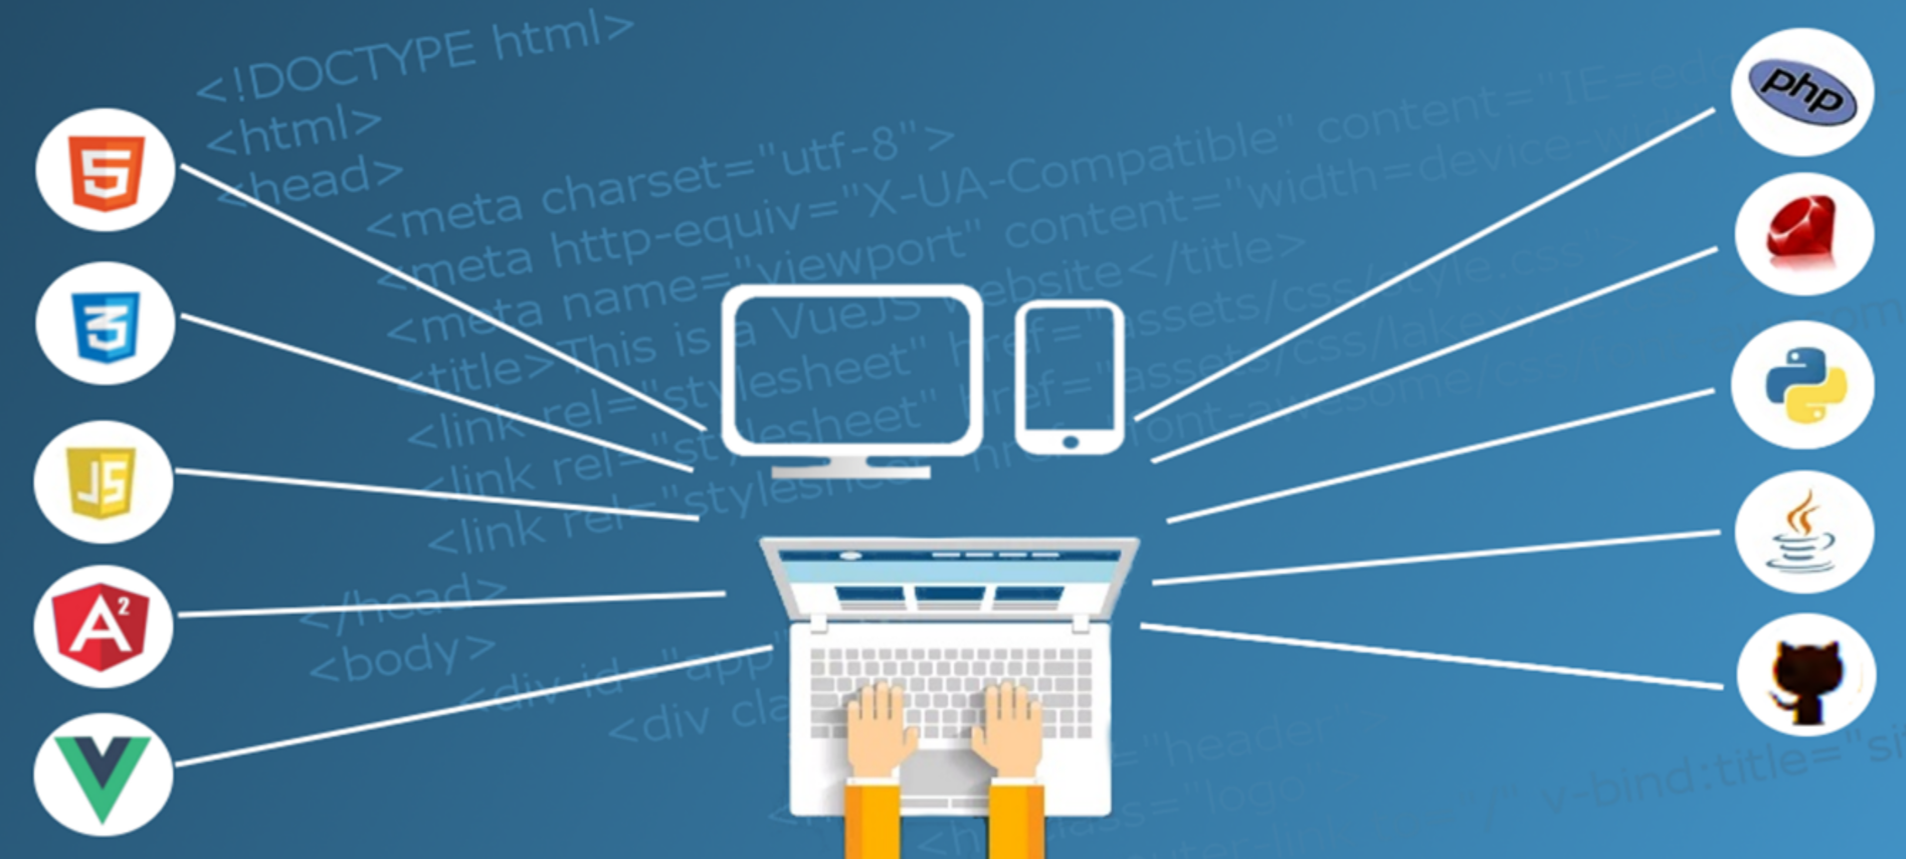
\includegraphics[width=.9\linewidth]{./Images/Chapter09/web-coding-olalekan-oladipupo-pixabay.png}
%\end{jazzgraphic*}



%----------
\section[Réseaux sociaux]{Réseaux sociaux}
\label{sec:IX.3}

\subsection[Découvrir la thématique]{Découvrir la thématique}
\label{sub:IX.3.1}


\subsubsection[Ancrage dans le réel]{Ancrage dans le réel}
\label{subsub:IX.3.1.1}

\overparagraph{Points-clés}

\begin{marginvideo}
	[\label{vid:IX.7}Réseaux sociaux.]%
	\movie[width=\marginparwidth,showcontrols]%
		{
\includegraphics[width=\marginparwidth]{./Images/Pictograms/film-strip-dark-electric-blue.png}}%
		{./Videos/Chapter09/vidIX-07-mooc-snt-social-networks.mp4}%
	\launchvideo{./Videos/Chapter09/vidIX-07-mooc-snt-social-networks.mp4}
\end{marginvideo}

\begin{jazzitemize}
\item La notion de réseau social est bien antérieure aux réseaux sociaux Internet,  elle est étudiée dès la fin du IXX\frup{e} siècle, et est un champ d'étude humaine qui se fonde sur des modèles informatiques.
\item On distingue la notion de communauté (personnes partageant des valeurs et des convictions communes) de la notion de société (personnes regroupées pour des raisons extérieures).
\item Le réseau social pour un individu a une taille maximale d'environ 150 personnes,  au-delà, sa perception est celle d'une foule.
\item Au sein d'un réseau, la chaîne des connaissances sociales liant une personne à n'importe quelle autre est généralement courte, toute personne est reliée à n'importe quelle autre par une chaîne de six maillons maximum ; cela est vrai même pour les très grands réseaux.
\item Il faut bien distinguer l'expérience de \textsc{Milgram} sur l'\href{https://fr.wikipedia.org/wiki/Exp\%C3\%A9rience_de_Milgram}{obéissance} de celle sur les \href{https://fr.wikipedia.org/wiki/\%C3\%89tude_du_petit_monde\#Exp\%C3\%A9riences_men\\%C3\%A9es_par_Milgram}{petits mondes} et distinguer cette idée du \href{https://fr.wikipedia.org/wiki/R\%C3\%A9seau_\%C2\%AB_petit_monde_\%C2\%BB}{concept mathématique} éponyme.
\end{jazzitemize}

%\sidegraphic{
\includegraphics[width=\linewidth]{./Images/Chapter09/wikipedia-logo-v2-fr.pdf}}{Wikimedia Foundation}%
\begin{margingraphic}{-20pt}
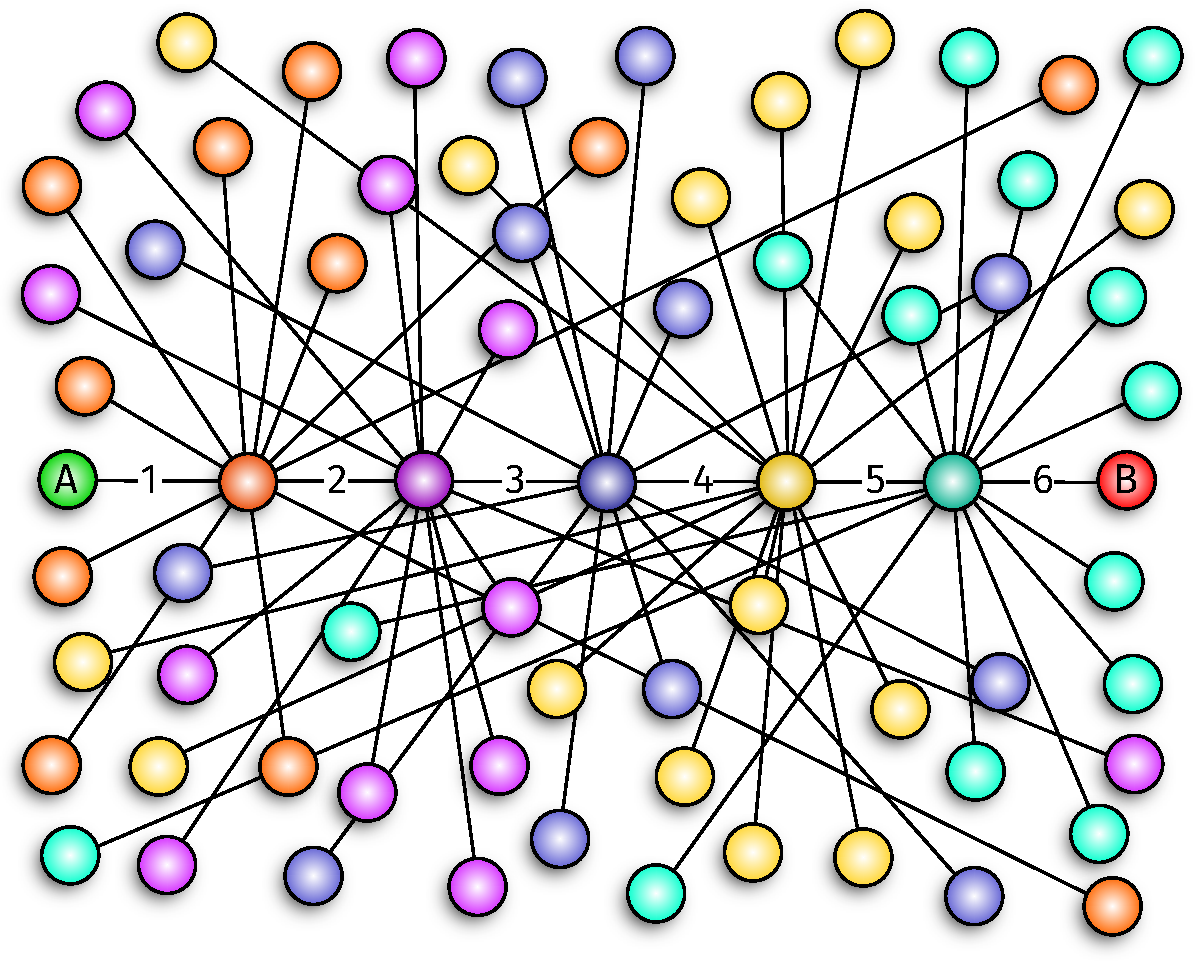
\includegraphics[width=\linewidth]{./Images/Chapter09/milgram-six-degrees-of-separation.pdf}
\caption{Illustration des six niveaux de séparation de la théorie des petits mondes.}
\end{margingraphic}


\overparagraph{Mots-clés}

\begin{jazzitemize}
\item Notion de \href{https://fr.wikipedia.org/wiki/Analyse_des_r\%C3\%A9seaux_sociaux}{réseau social}.
\item \href{https://interstices.info/routage-dans-les-petits-mondes/}{Routage dans les petits mondes}.
\item Notion de \href{https://fr.wikipedia.org/wiki/M\%C3\%A9dia_social}{média social}.
\end{jazzitemize}

\overparagraph{Ce que dit le programme}

\begin{tcolorbox}[title={Introduction}, toprule=0pt, leftrule=0pt, rightrule=0pt, arc=0pt, fonttitle=\scshape\boxtitlefont,
                  colbacktitle=white, coltitle=firstcolor, colframe=firstcolor, colback=firstcolor!10,
                  breakable, enhanced jigsaw]
Les réseaux sociaux sont des applications basées sur les technologies du Web qui offrent un service de mise en relation d’internautes pour ainsi développer des communautés d’intérêts.

\end{tcolorbox}

\begin{tcolorbox}[title={Impacts sur les pratiques humaines}, toprule=0pt, leftrule=0pt, rightrule=0pt, arc=0pt,
                  fonttitle=\scshape\boxtitlefont,
                  colbacktitle=white, coltitle=firstcolor, colframe=firstcolor, colback=firstcolor!10,
                  breakable, enhanced jigsaw]
Le développement des réseaux sociaux introduit un nouveau type de liens sur le Web, qui ne relève pas de l’hypertexte : il s’agit de l’abonnement à des relations/des amis et de la possibilité de recommander de l’information en fonction du réseau ainsi constitué.

L’objectif annoncé des applications de réseautage social est de mettre les individus en relation les uns avec les autres. Quelle est la réalité ? L’\emph{expérience de Milgram} (1967) semble indiquer la constitution de « \emph{petits mondes} » où chacun est au plus à six liens de distance d’un autre. Peut-on éviter les phénomènes de communautés liés à des recommandations se renforçant les unes les autres pouvant aller jusqu’à un appauvrissement de la pensée critique ? Ces questions font référence au concept de \textit{bonding} (renforcement de liens existants au sein d’un même groupe) versus \textit{bridging} (construction de nouveaux liens non redondants).

Les affaires de fuite de données personnelles mettent en avant les questions liées aux modèles économiques des applications de réseautage social symbolisés par le slogan « \textit{quand c’est gratuit, c’est vous le produit} ».

Les réseaux sociaux peuvent être le support d’un \emph{harcèlement numérique}, par le biais de photographies partagées sans consentement ou impossibles à retirer, par la diffusion de fausses nouvelles, de dénonciations ou de calomnies. Des pratiques, des outils et des services permettent de se protéger, lutter et dénoncer de tels agissements.
\end{tcolorbox}


\subsubsection[Volet historique]{Volet historique}
\label{subsub:IX.3.1.2}

À la fin des années 1890, Émile \textsc{Durkheim} et Ferdinand \textsc{Tönnies} ont laissé entrevoir l'idée de réseaux sociaux dans leurs théories et leurs recherches sur les groupes sociaux. \textsc{Tönnies} a fait valoir que les groupes sociaux peuvent exister en tant que liens sociaux personnels et directs liant des individus partageant des valeurs et des convictions communes (« communauté »), ou des liens sociaux impersonnels, formels et instrumentaux (« société »). \textsc{Durkheim} a donné une explication non individualiste des faits sociaux, affirmant que les phénomènes sociaux surviennent lorsque les individus en interaction constituent une réalité qui ne peut plus s'expliquer à l'aide des propriétés d'acteurs individuels.

\begin{margingraphic}
\Centering
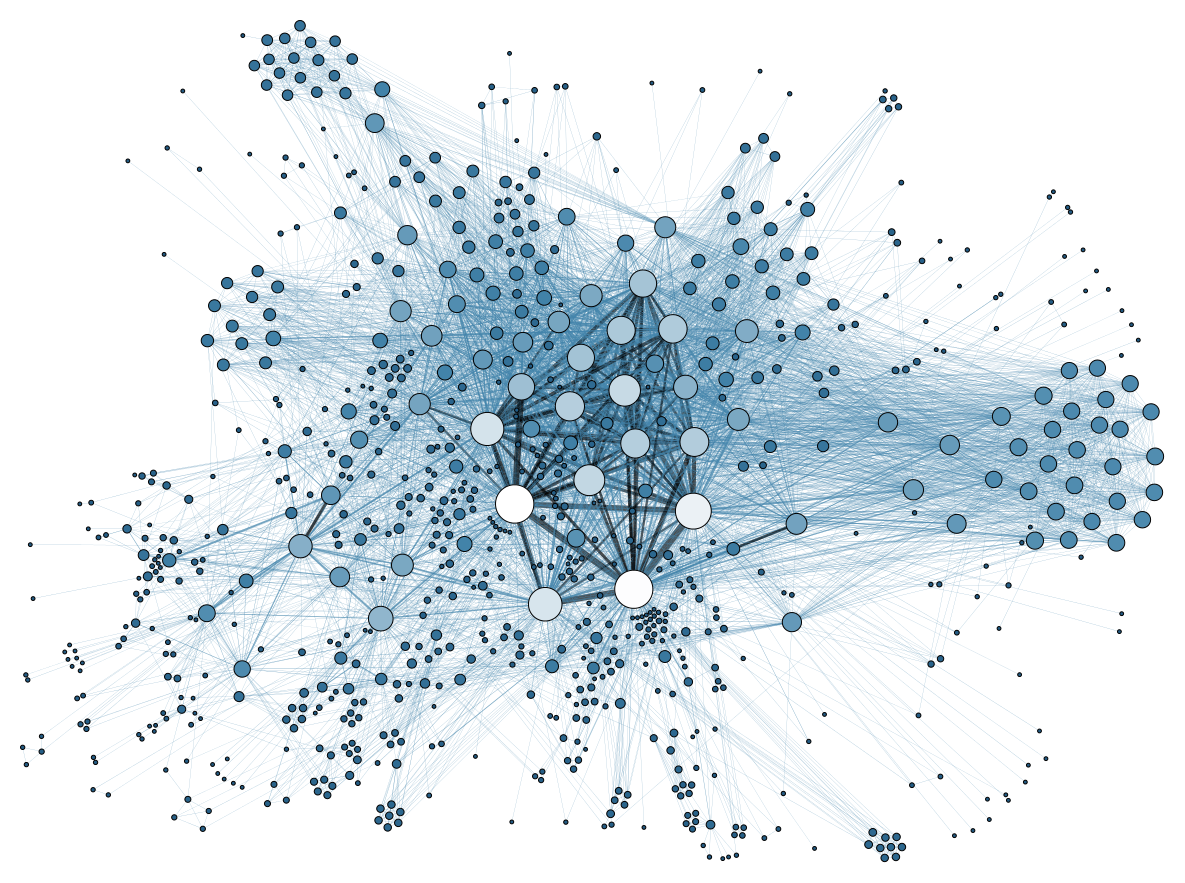
\includegraphics[width=\linewidth]{./Images/Chapter09/social-network-analysis-visualization.png}
\caption{Visualisation d'un réseau social.}
\end{margingraphic}

Des développements majeurs dans le domaine sont observés dans les années 1930 par plusieurs groupes de psychologie, d'anthropologie et de mathématiques. En psychologie, dans les années 1930, Jacob L. \textsc{Moreno} a commencé l’enregistrement et l’analyse systématiques des interactions sociales en petits groupes, en particulier les salles de classe et les groupes de travail. En anthropologie, les travaux théoriques et ethnographiques sont à la base de la théorie des réseaux sociaux.  En sociologie, les travaux de Talcott \textsc{Parsons} (dans les années 1930) ont ouvert la voie à une approche relationnelle de la compréhension de la structure sociale.

Dans les années 1970, un nombre croissant d'érudits ont travaillé pour combiner les différentes pistes et traditions. Un des groupes était constitué du sociologue Harrison \textsc{White} et de ses étudiants du département des relations sociales de l’Université de Harvard. Stanley \textsc{Milgram}, qui développa la thèse des « six degrés de séparation », était également au sein du département des relations sociales de Harvard à l'époque. Mark \textsc{Granovetter} et Barry \textsc{Wellman} font partie des anciens élèves de \textsc{White} qui ont élaboré et défendu l'analyse des réseaux sociaux.

À partir de la fin des années 1990, des sociologues, des politologues et des physiciens tels que Duncan J. \textsc{Watts}, Albert-László \textsc{Barabási}, Peter \textsc{Bearman}, Nicholas A. \textsc{Christakis} et James H. \textsc{Fowler}, ainsi que d’autres, ont analysé les réseaux sociaux. Les « traces numériques » et toutes les données émergentes disponibles sur les réseaux sociaux en ligne ont permis de créer de nouveaux modèles et méthodes d'analyse.

\overparagraph*{Ce que dit le programme}

\begin{tcolorbox}[title={Repères historiques}, toprule=0pt, leftrule=0pt, rightrule=0pt, arc=0pt,
                  fonttitle=\scshape\boxtitlefont,
                  colbacktitle=white, coltitle=firstcolor, colframe=firstcolor, colback=firstcolor!10,
                  breakable, enhanced jigsaw]
\begin{jazzitemize}
\item 1995 : \textsc{Classmates} est l’un des premiers réseaux sociaux qui permettent aux étudiants de rester en relation.
\item 2003 : apparition de \textsc{Myspace}, aujourd’hui en perte de vitesse et de \textsc{LinkedIn} (racheté depuis par \textsc{Microsoft}), à vocation professionnelle.
\item 2004 : apparition de \textsc{Facebook}, d’abord réservé aux étudiants de l’université Harvard, puis ouvert au grand public en 2006.   
\item 2006 : apparition de \textsc{Twitter}, qui permet l’échange de courts messages, limités au départ à 140 puis à 280 caractères (on parle de microblogage).
\item 2009 : lancement de la messagerie instantanée \textsc{WhatsApp} (rachetée depuis par \textsc{Facebook}) qui se substitue à l’utilisation des SMS et MMS chez beaucoup d’utilisateurs.
\item 2010 : arrivée d’\textsc{Instagram} (racheté depuis par \textsc{Facebook}), qui permet le partage de photos et de vidéos. 
\item 2011 : début de \textsc{Snapchat} qui permet, sur plateformes mobiles, le partage de photos et de vidéos, avec une limitation de durée.
\item 2018 : on estime à 3,2 milliards le nombre d’utilisateurs actifs des réseaux sociaux.
\end{jazzitemize}

En 2018, les réseaux sociaux utilisés en France sont états-uniens, toutefois il en existe bien d’autres : en Chine, par exemple, apparaît en 2009 l’application de microblogage \textsc{Weibo} avec plus de 350 millions d’utilisateurs actifs en 2018 ; en 2012 naît l’application de messagerie \textsc{Weixin} (développée par \textsc{Tencent}) qui compte en 2018 plus d’un milliard de comptes utilisateurs.
\end{tcolorbox}


\subsubsection[Explication des notions]{Explication des notions}
\label{subsub:IX.3.1.3}

\overparagraph{Idées-forces}

\begin{jazzitemize}
\item Les réseaux sociaux s'étudient à l'aide de graphes, un modèle mathématique majeur (relations entre des personnes, entre des lieux, entre des actions, etc.).
\item Beaucoup de problèmes concrets peuvent se ramener à des questions sur des graphes avec, selon les cas, des solutions connues ou non, calculables facilement ou pas.
\item Ce qui nous est accessible sur les réseaux sociaux est présélectionné par des algorithmes de recommandation, par exemple en lien avec nos recherches précédentes. Cela biaise le résultat et tend à restreindre le champ de ce qui est accessible.
\end{jazzitemize}

\overparagraph{Mots-clefs}

\begin{jazzitemize}
\item Notion de \href{https://fr.wikipedia.org/wiki/Th\%C3\%A9orie_des_graphes}{graphe}.
\item \href{https://fr.wikipedia.org/wiki/Syst\%C3\%A8me_de_recommandation}{Systèmes de recommandation}.
\end{jazzitemize}

\overparagraph{Ce que dit le programme}

\begin{tcolorbox}[title={Données et information}, toprule=0pt, leftrule=0pt, rightrule=0pt, arc=0pt,
                  fonttitle=\scshape\boxtitlefont,
                  colbacktitle=white, coltitle=firstcolor, colframe=firstcolor, colback=firstcolor!10,
                  breakable, enhanced jigsaw]
Les différents réseaux sociaux permettent l’échange d’informations de natures différentes : textes, photos, vidéos. Certains limitent strictement la taille des informations, d’autres autorisent la publication, mais de façon limitée dans le temps. Certains permettent l’adjonction d’applications tierces (greffons ou \textit{plug-ins}) qui peuvent ajouter des fonctionnalités supplémentaires.

Toutes les applications de réseautage social utilisent d’importantes bases de données qui gèrent leurs utilisateurs, l’ensemble des données qu’ils sont amenés à partager, mais aussi celles qu’ils consentent à fournir (sans toujours le savoir), y compris sur leur vie personnelle.
\end{tcolorbox}

\begin{tcolorbox}[title={Algorithmes et programmes}, toprule=0pt, leftrule=0pt, rightrule=0pt, arc=0pt,
                  fonttitle=\scshape\boxtitlefont,
                  colbacktitle=white, coltitle=firstcolor, colframe=firstcolor, colback=firstcolor!10,
                  breakable, enhanced jigsaw]
De très nombreux algorithmes sont mis en œuvre par les applications de réseautage social.
Toutes les applications s’appuient sur la mise en relation avec des internautes membres du réseau, relations ou amis communs : des algorithmes opérant sur les \emph{graphes} et les bases de données sont au cœur de ces services.

À l’aide d’algorithmes de recommandation, les réseaux sociaux suggèrent aux utilisateurs des amis, des contenus, des annonces promotionnelles. Ils permettent aussi aux plateformes sociales d’étudier les comportements de leurs utilisateurs à des fins commerciales, politiques ou d’amélioration du service.
\end{tcolorbox}


\overparagraph{Web-conférence}

\begin{marginvideo}
	[\label{vid:IX.8}Réseaux sociaux.]%
	\movie[width=\marginparwidth,showcontrols]%
		{
\includegraphics[width=\marginparwidth]{./Images/Pictograms/film-strip-dark-electric-blue.png}}%
		{./Videos/Chapter09/vidIX-08-conf-snt-social-networks-unknown.mp4}%
	\launchvideo{./Videos/Chapter09/vidIX-08-conf-snt-social-networks-unknown.mp4}
\end{marginvideo}

\textsc{Class'Code} \textsc{Pays-de-Loire} a organisé des conférences qui abordent les sept thématiques du programme SNT. Leur objectif est de fournir une vue d’ensemble et de poser les bases nécessaires à l’appropriation de ces grands domaines sous deux angles définis par le programme :
\begin{itemize}
\item une présentation historique (30 à 45 minutes) : grandes étapes de création/développement, acteurs majeurs, contexte général, histoire des idées et mise en contexte suffisamment fiable pour être réutilisée en cours ;
\item des exemples concrets de ce qui est étudié ou produit dans ces domaines et une réflexion sur les besoins et enjeux actuels et à venir à travers un débat (45 à 60 minutes) qui laisse la parole à des personnes travaillant dans ces champs de spécialité  (chercheurs, enseignants, étudiants, entreprises...), que ce soit en recherche ou en entreprise.
\end{itemize}

La conférence sur les \textit{réseaux sociaux} a eu lieu le 5 mars 2019 dans le cadre du projet \textsc{Class'Code} à l’Université de Nantes. Elle a été retransmise en ligne et est maintenant disponible sur \textsc{YouTube}.

\begin{jazzgraphic*}
\begin{tikzpicture}[remember picture, overlay]
\node[anchor=east, inner sep=0pt, rotate=-90, xshift=0pt, yshift=(\linewidth+6pt)] 
	at (0,0) {\scriptsize\faCopyright\space Gerd Altmann \textit{via} \href{https://pixabay.com}{Pixabay}};
\end{tikzpicture}%
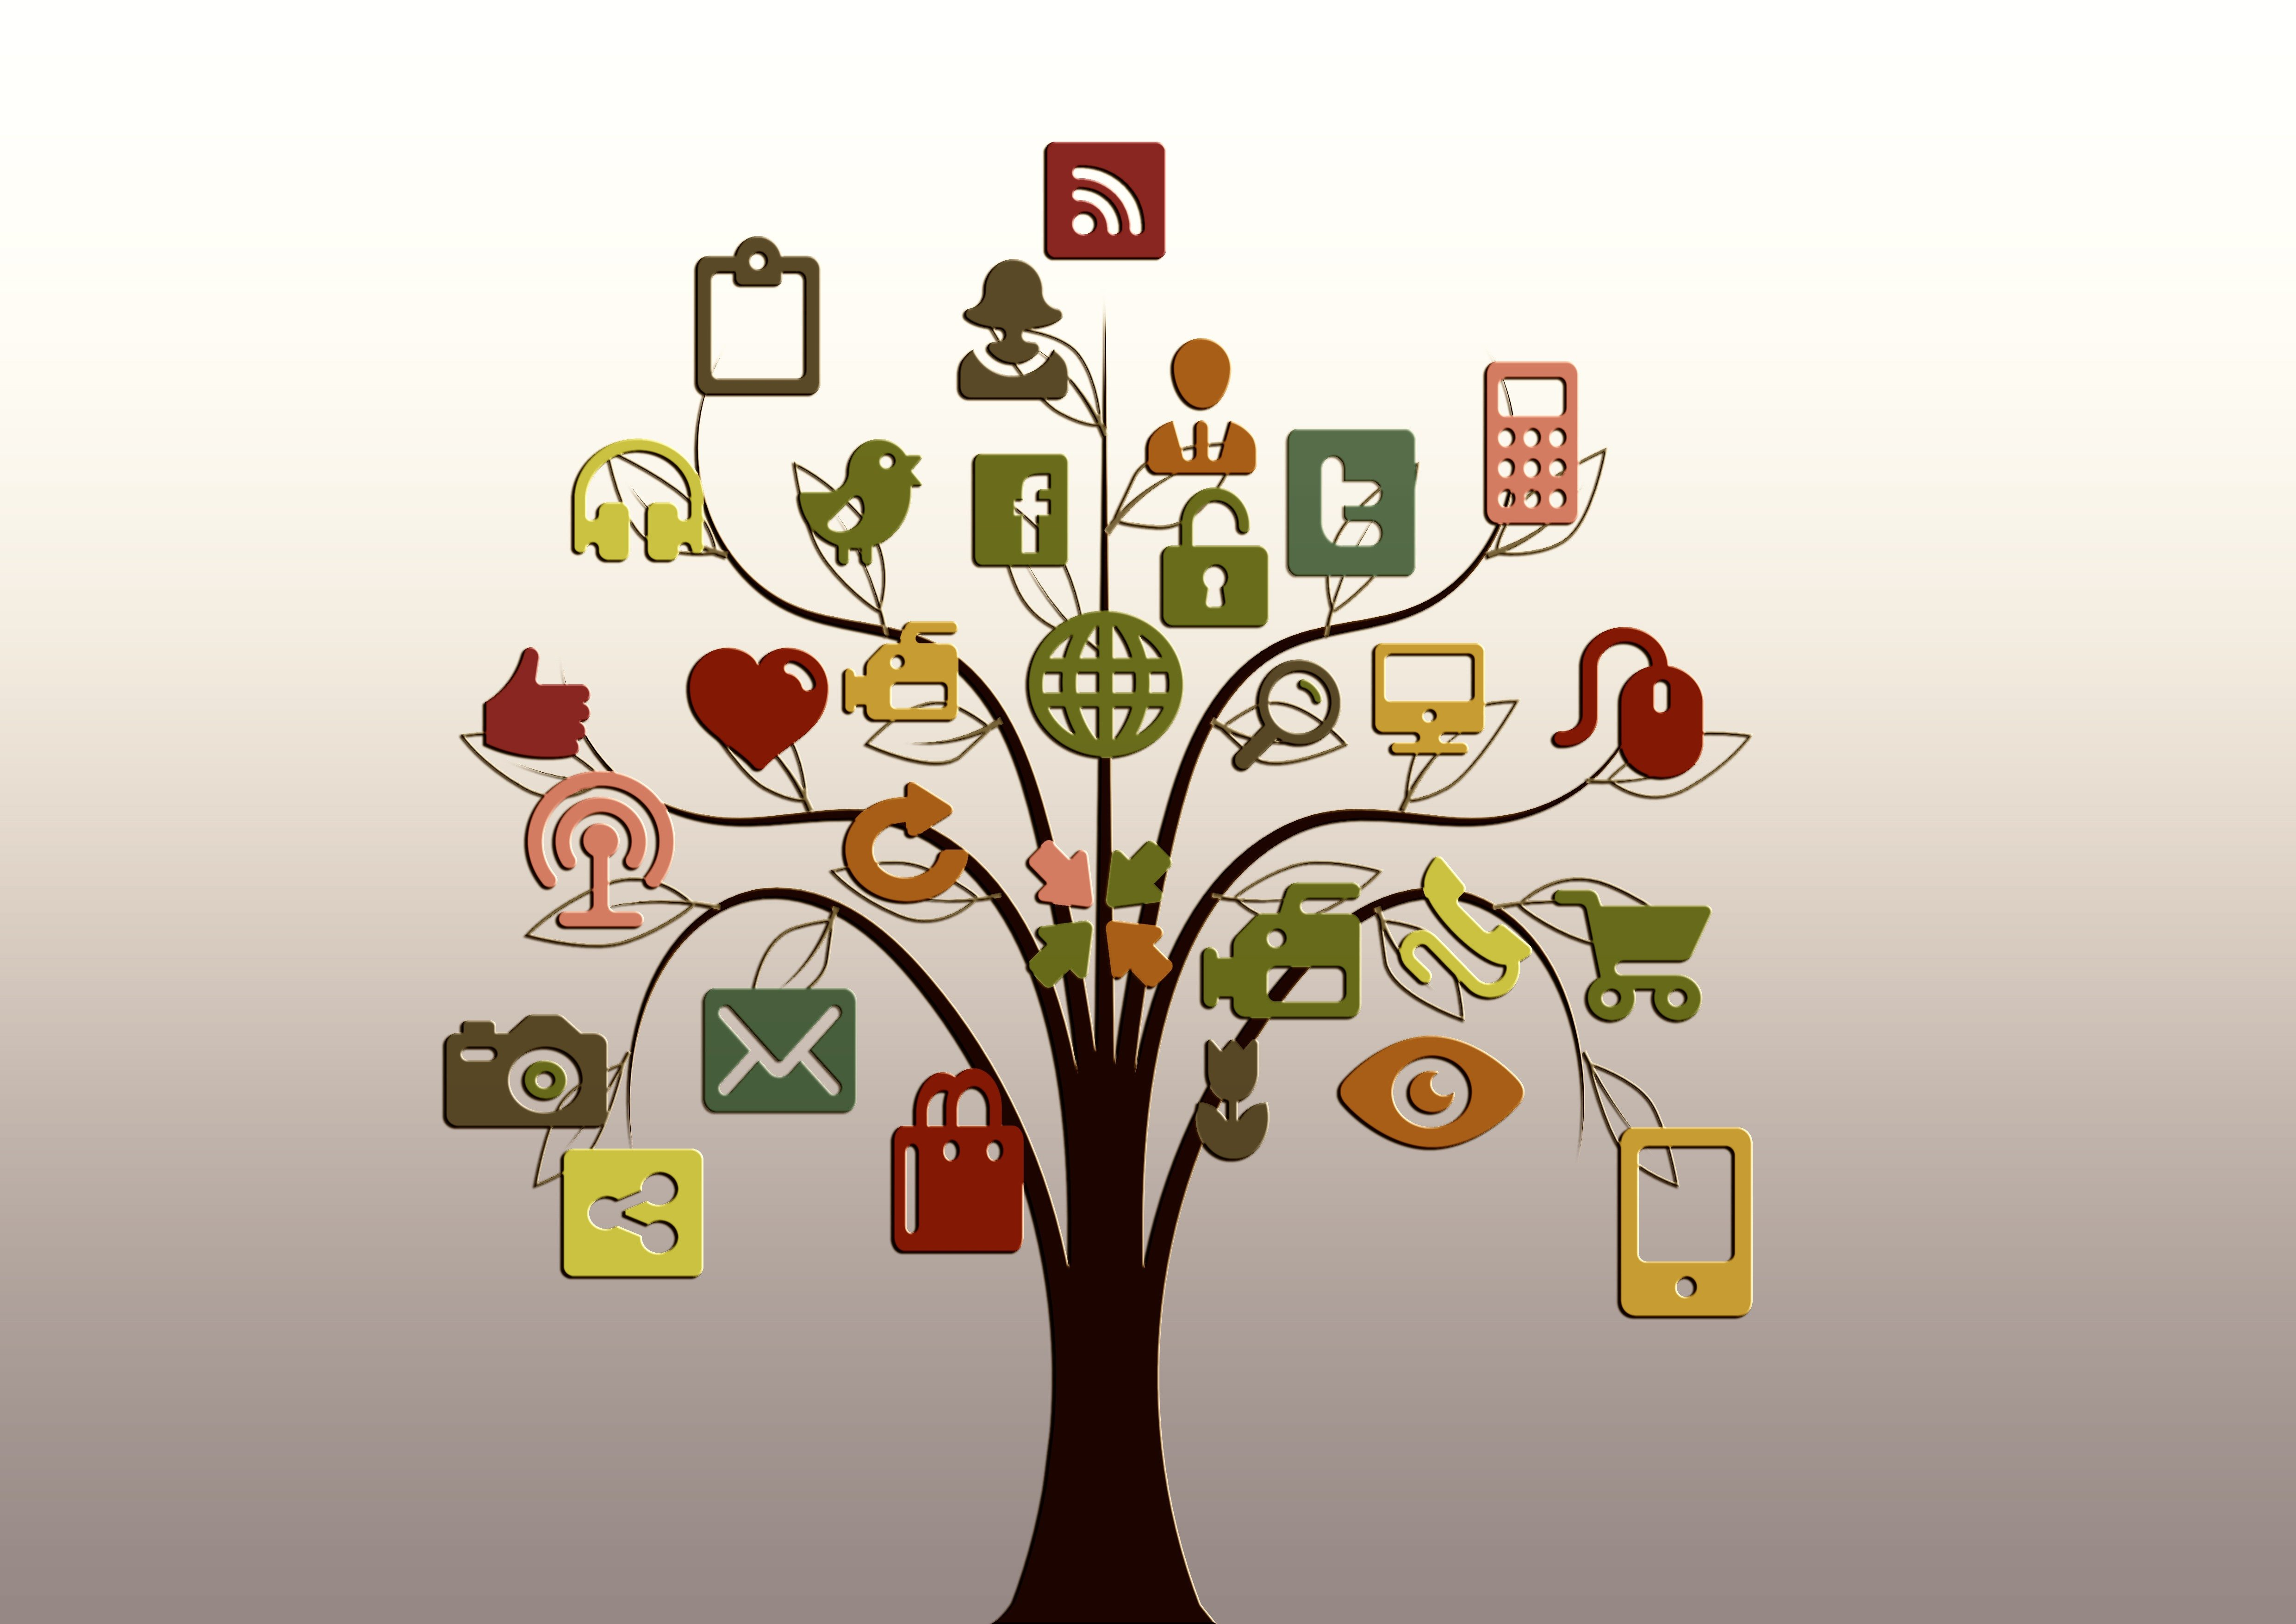
\includegraphics[width=\linewidth]{./Images/Chapter09/tree-gerd-altmann-pixabay.jpg}%
%\begin{tikzpicture}[remember picture, overlay]
%\node[anchor=west, inner sep=0pt, rotate=90, xshift=0pt, yshift=(\linewidth+6pt)] 
%	at (0,0) {\scriptsize\faCopyright\space Gerd Altmann via \href{https://pixabay.com}{Pixabay}};
%\end{tikzpicture}%
\end{jazzgraphic*}

\vspace{4pt}

\begin{gofurther}{Ressources complémentaires}
\lightbf{Se former}
\begin{itemize}\jazzitem
\item Pour les enseignants : la \href{https://magistere.education.fr/dgesco/}{conférence de Christine \textsc{Gaubert-Macon} sur le Web, Internet et les réseaux sociaux}, lors des formations nationales, accès par m@gistere (réservé aux enseignant·e·s).
\item Présentation du \href{https://pixees.fr/du-web-aux-reseaux-sociaux/}{Web au réseaux sociaux} par Fabien \textsc{Gandon}.
\item Une \href{https://interstices.info/dossier/snt-reseaux-sociaux/}{sélection d'articles} du site \textsc{Interstices}.
\end{itemize}

\vspace{2pt}
\lightbf{Ouvrages}
\begin{itemize}\jazzitem
\item Fabien \textsc{Tarissan} (2019) « Au cœur des réseaux : des sciences aux citoyens », Édition le Pommier. Il traite de science, plus particulièrement des réseaux (informatiques et autres), des algorithmes qui y opèrent et de l'impact qu'ils ont sur notre manière de nous informer en ligne (\textit{fake news}, publicité ciblée, données personnelles, etc.), et de l'économie sous-jacente.
\end{itemize}

\vspace{2pt}
\lightbf{Créer son cours}
\begin{itemize}\jazzitem
\item Des animations intéressantes sur les réseaux sociaux et le web en général (les \textit{cookies}...) sur le site d'\href{https://donottrack-doc.com/fr/episodes/}{Arte}.
\item La ressource librement utilisable « \href{https://www.isoloir.net/}{isoloir} » propose une activité sur l'identité numérique et la liberté d'expression, à faire en classe en semi-autonomie, ces \href{https://pixees.fr/informatique-et-societe-du-jeu-serieux-au-document-pedagogique/}{documents} sont librement réutilisables.
\item Dynamique des groupes de partage dans les réseaux sociaux : des recherches ont analysé comment les utilisateurs des réseaux sociaux font et défont les communautés au fil du temps, voir cet article en français : \href{https://hal.archives-ouvertes.fr/hal-00815680}{De la difficulté de garder ses amis (quand on a des ennemis) !}
\item Comment fonctionnent les systèmes de recommandation (article du Blog Binaire du Monde.fr) revue en ligne \textsc{Binaire} sur le site du Monde, 27 décembre 2016.
\item \href{https://interstices.info/les-systemes-de-recommandation-categorisation/}{Les systèmes de recommandation : une catégorisation}, Elsa Negre, \textsc{Interstices}, 20 septembre 2018.
\item \href{https://www.arte.tv/fr/videos/RC-017841/dopamine/}{Dopamine}, une websérie sur \textsc{Arte} qui décortique notre addiction aux applis : \textsc{Tinder}, \textsc{Facebook}, \textsc{Candy Crush}, \textsc{Instagram}, \textsc{YouTube}, \textsc{Snapchat}, \textsc{Uber}, \textsc{Twitter}, Léo Favier, Coproduction ARTE France, Les Bons Clients, Réseau Canopé, 8 vidéos.
\end{itemize}
\end{gofurther}


\subsection[Réaliser des activités]{Réaliser des activités}
\label{sub:IX.3.2}

\overparagraph*{Exemple d'activités}

Les activités proposées\caution[t]<firstcolor>{%
Toutes les fiches actuellement collectées sont disponibles à l'URL : \url{http://tinyurl.com/yx9qce8s} et on peut aussi proposer des activités.}{Note de la rédaction}
sont disponibles sous forme de fiches à télécharger (format ODT de la suite bureautique libre \textsc{LibreOffice}).

\begin{jazzitemize}
\item \textdoc{./Documents/Chapter09/cardIX-15-snt-social-net-david-roche.odt}{Faire des recherches sur différents réseaux sociaux}.
\item \textdoc{./Documents/Chapter09/cardIX-16-snt-social-net-graphs-david-roche.odt}{Possibilité de modéliser les réseaux sociaux par des graphes}.
\item \textdoc{./Documents/Chapter09/cardIX-17-snt-social-net-milgram-david-roche.odt}{Découverte de la notion de « petit monde »}.
\end{jazzitemize}

\noindent Fiche d'activité élève :
\begin{jazzitemize}
\item \pdfdoc{./Documents/Chapter09/activityIX-04-snt-social-net-graphs.pdf}{Tracer un graphe de réseau social}.
\end{jazzitemize}

%\overparagraph{Ce que propose le programme}

\begin{tcolorbox}[title={Ce que propose le programme}, toprule=0pt, leftrule=0pt, rightrule=0pt, arc=0pt,
                  fonttitle=\scshape\boxtitlefont,
                  colbacktitle=white, coltitle=firstcolor, colframe=firstcolor, colback=firstcolor!10,
                  breakable, enhanced jigsaw]
\begin{jazzitemize}
\item Construire ou utiliser une représentation du graphe des relations d’un utilisateur. S’appuyer sur la densité des liens pour identifier des groupes, des communautés.   
\item Sur des exemples de graphes simples, en informatique débranchée, étudier les notions de rayon, diamètre et centre d’un graphe, de manière à illustrer la notion de « petit monde ». 
\item Comparer les interfaces et fonctionnalités de différents réseaux sociaux.
\item Dresser un comparatif des formats de données, des possibilités d’échange ou d’approbation (bouton like), de la persistance des données entre différents réseaux sociaux.
\item Analyser les paramètres d’utilisation d’un réseau social. Analyser les autorisations données aux applications tierces.
\item Discuter des garanties d’authenticité des comptes utilisateurs ou des images.
\item Lire et expliquer les conditions générales d’utilisation d’un réseau social.
\item Consulter le site \url{nonauharcelement.education.gouv.fr}.
\end{jazzitemize}
\end{tcolorbox}

\begin{jazztable*}
\caption{\label{tab:IX.3}Réseaux sociaux : compétences attendues chez les élèves.}
\Centering
\begingroup
\small
\renewcommand*{\arraystretch}{1.6}
\rowcolors{2}{tableLineOne}{tableLineTwo}
\begin{tabularx}{\linewidth}{lX}
\rowcolor{secondcolor}
\multicolumn{2}{c}{\Gape[6pt]{\textcolor{white}{\textbf{Internet}}}} \\
\rowcolor{firstcolor}
\multicolumn{1}{c}{\scshape\titlingfont\textcolor{white}{Contenus}} 
	&	\multicolumn{1}{c}{\scshape\titlingfont\textcolor{white}{Capacités attendues}} \\
Réseaux sociaux existants
  & Distinguer plusieurs réseaux sociaux selon leurs caractéristiques,\newline y compris un ordre de grandeur de leurs nombres d’abonnés.\newline
    Paramétrer des abonnements pour assurer la confidentialité\newline de données personnelles. \\
Modèle économique des réseaux sociaux 
  & Identifier les sources de revenus des entreprises de réseautage social.\\
Rayon, diamètre et centre d’un graphe
  & Déterminer ces caractéristiques sur des graphes simples.\\
Notion de « petit monde » (\textsc{Milgram})
  & Décrire  comment l’information présentée par les réseaux sociaux\newline est conditionnée par le choix préalable de ses amis. \\
Harcèlement numérique
  & Analyser l’\href{https://www.legifrance.gouv.fr/codes/id/LEGIARTI000037289658/2018-08-06/}{article 222-33-2-2} du code pénal. \\
\end{tabularx}%
\endgroup
\end{jazztable*}



%----------
\section[Enjeux environnementaux]{Enjeux environnementaux}
\label{sec:IX.4}

L’enseignement des sciences numériques et technologie doit également permettre aux élèves de comprendre le poids croissant du numérique et les enjeux qui en découlent. Pour cette raison, ont été récoltées des ressources au sujet du numérique et de l'environnement afin d'offrir aux enseignants de la matière pour une prise de conscience par les élèves des impacts environnementaux du numérique, que ce soit pour la fabrication, la consommation et le recyclage.

Suite à la présentation de la thématique, une intervention de Françoise \textsc{Berthoud} est proposée issue des conférences \textit{Comprendre et Agir}, Inria, juin 2018. Ensuite, des fiches de synthèse des ressources récoltées donnent quelques pistes de réflexion avec des exemples con\-crets et des schémas éloquents. Toutes les références à ces ressources sont données au fur et à mesure, ne pas hésiter pas à aller les consulter. Cette partie est en construction permanente au vu des impacts grandissant du numérique dans l'environnement.



\subsection[Découvrir la thématique]{Découvrir la thématique}
\label{sub:IX.4.1}

Il est important de comprendre\caution[t]<secondcolor>{Attention, les données sur ce sujet sont plus ou moins disponibles, en général imprécises mais surtout très évolutives. Toutes les sources de cette séquence sont précisées.}{Avertissement}
 les impacts environnementaux du numérique, en pensant notamment aux trois facettes suivantes :
\begin{itemize}
\item fabrication (extraction des ressources, production, transport),
\item utilisation (consommation électrique et de données),
\item recyclage.
\end{itemize}

Qu'entend-on par numérique dans cette séquence ? On parle ici des équipements terminaux (PC, \textit{laptop}, tablette, \textit{smartphone}, mobile, etc.), des écrans (moniteurs), des serveurs et de leur environnement, des équipements réseaux passifs et actifs (filaire, Wi-Fi, GSM, xG, etc.) et de la télévision numérique ou connectée.

\subsubsection[Ancrage dans le réel]{Ancrage dans le réel}
\label{subsub:IX.4.1.1}

\overparagraph{Points-clefs}

\begin{jazzitemize}
\item Le secteur du numérique a un taux de croissance particulièrement important (+8\,\% par an). À l'échelle mondiale, il est responsable d’environ 10\,\% de la consommation électrique, tout cela sans compter les objets connectés et les systèmes embarqués.   
\item Au niveau planétaire, les technologies du numérique sont responsables d’environ 4\,\% des émissions de gaz à effet de serre (GES), soit plus que celles engendrées par l’aviation civile !
\item L’extraction et le raffinage des métaux puis la production des composants nécessaires à la réalisation des équipements électroniques ainsi que leur recyclage, lorsqu’il n’est pas fait dans les règles de l’art, sont aussi des sources considérables de pollution.
\item Le numérique est à l'origine de gros problèmes sanitaires dans plusieurs pays africains et asiatiques où des sites de recyclages « informels » inondent les sols, air et eau de métaux lourds et de substances chimiques très polluantes.
\item L'extraction des métaux est également responsable de conflits d'accès à l'eau et de conflits armés ; par exemple en Afrique du Nord, en Amérique du Sud, en République Démocratique du Congo...
\item Le développement des technologies numériques participe aussi de manière importante à l’épuisement de certaines ressources.
\item Le recyclage représente un espoir pour amortir l’épuisement des ressources, mais actuellement les taux de récupération des métaux dans les appareils électroniques sont faibles  : sur la cinquantaine de métaux présents dans un \textit{smartphone}, dans le meilleur des cas seuls vingt sont recyclés.
\item Sans remettre en cause les apports réels des technologies numériques dans la société, participant notamment à notre confort --- à savoir communication, diffusion des savoirs, technologie GPS, etc. ---, il est important de garder à l’esprit les coûts environnementaux associés (pollution, destruction des écosystèmes, réchauffement climatique, etc.) dont la croissance exponentielle s'ajuste sur notre propre consommation exponentielle du numérique.
\end{jazzitemize}

\noindent Source : \href{https://www.lemonde.fr/blog/binaire/2019/06/17/plus-d-ambitions-climatiques/}{Plus d’ambitions climatiques !} Françoise \textsc{Berthoud} (\textsc{Cnrs}), Jac\-ques \textsc{Combaz} (\textsc{Cnrs}) et Kevin \textsc{Marquet} (Inria), Binaire, 17 juin 2019.

\overparagraph{Mots-clefs}

\begin{jazzitemize}
\item \lightbf{Centre de données -- \textit{Data center}} --- Un centre de données (en anglais \textit{data center} ou \textit{data centre}) est un lieu (et un service) regroupant des équipements constituants du système d’information d'une ou plusieurs entreprise(s) (\href{https://fr.wikipedia.org/wiki/Ordinateur_central}{ordinateurs centraux}, serveurs, \href{https://fr.wikipedia.org/wiki/Baie_de_stockage}{baies de stockage}, équipements réseaux et de télécommunications, etc.) [\href{https://fr.wikipedia.org/wiki/Centre_de_donn\%C3\%A9es}{\faWikipediaW}].
\item \lightbf{Effet rebond} --- D’une manière très générale, l’effet rebond, encore appelé \href{https://fr.wikipedia.org/wiki/Paradoxe_de_Jevons}{paradoxe de Jevons}, peut être défini comme « l’augmentation de consommation liée à la réduction des limites à l’utilisation d’une technologie, ces limites pouvant être monétaires, temporelles, sociales, physiques, liées à l’effort, au danger, à l’organisation… ». Il en découle le corollaire suivant : les économies d’énergie ou de ressources initialement prévues par l’utilisation d’une \href{https://fr.wikipedia.org/wiki/Nouvelles_technologies}{nouvelle technologie} [plus efficace ou performante] sont partiellement ou complètement compensées à la suite d'une adaptation du comportement de la société. Il a une grande importance pour l'établissement, l'évaluation et la mise à jour de stratégies et politiques énergétiques [d'après \href{https://fr.wikipedia.org/wiki/Effet_rebond_(\%C3\%A9conomie)}{\faWikipediaW}]. Un exemple d'effet rebond : les batteries des \textit{smartphones} gagnent en autonomie ce qui permet aux développeurs de proposer des applications plus gourmandes en énergie.
\item \lightbf{\textit{Streaming}} --- Très utilisé sur Internet et sur les réseaux de téléphonie mobile, le \textit{streaming} permet la lecture d'un flux audio ou vidéo (cas de la vidéo à la demande) à mesure qu'il est diffusé. Il s'oppose ainsi à la diffusion par téléchargement de fichiers qui nécessite de récupérer l'ensemble des données d'un morceau ou d'un extrait vidéo avant de pouvoir l'écouter ou le regarder [\href{https://fr.wikipedia.org/wiki/Streaming}{\faWikipediaW}].
\item \lightbf{Obésitiel} --- Néologisme désignant un logiciel qui utilise beaucoup de ressources physiques.
\item \lightbf{Obsolescence} --- L'obsolescence est le fait pour un produit d'être dépassé et donc de perdre une partie de sa valeur d'usage en raison de la seule évolution \href{https://fr.wikipedia.org/wiki/Technique}{technique} (on parle alors d'« obsolescence technique ») ou de la \href{https://fr.wikipedia.org/wiki/Tendance_(mode)}{mode} (on utilise alors plutôt le mot « démodé »), même s'il est en parfait état de fonctionnement [\href{https://fr.wikipedia.org/wiki/Obsolescence}{\faWikipediaW}].
\end{jazzitemize}

\begin{jazzgraphic*}
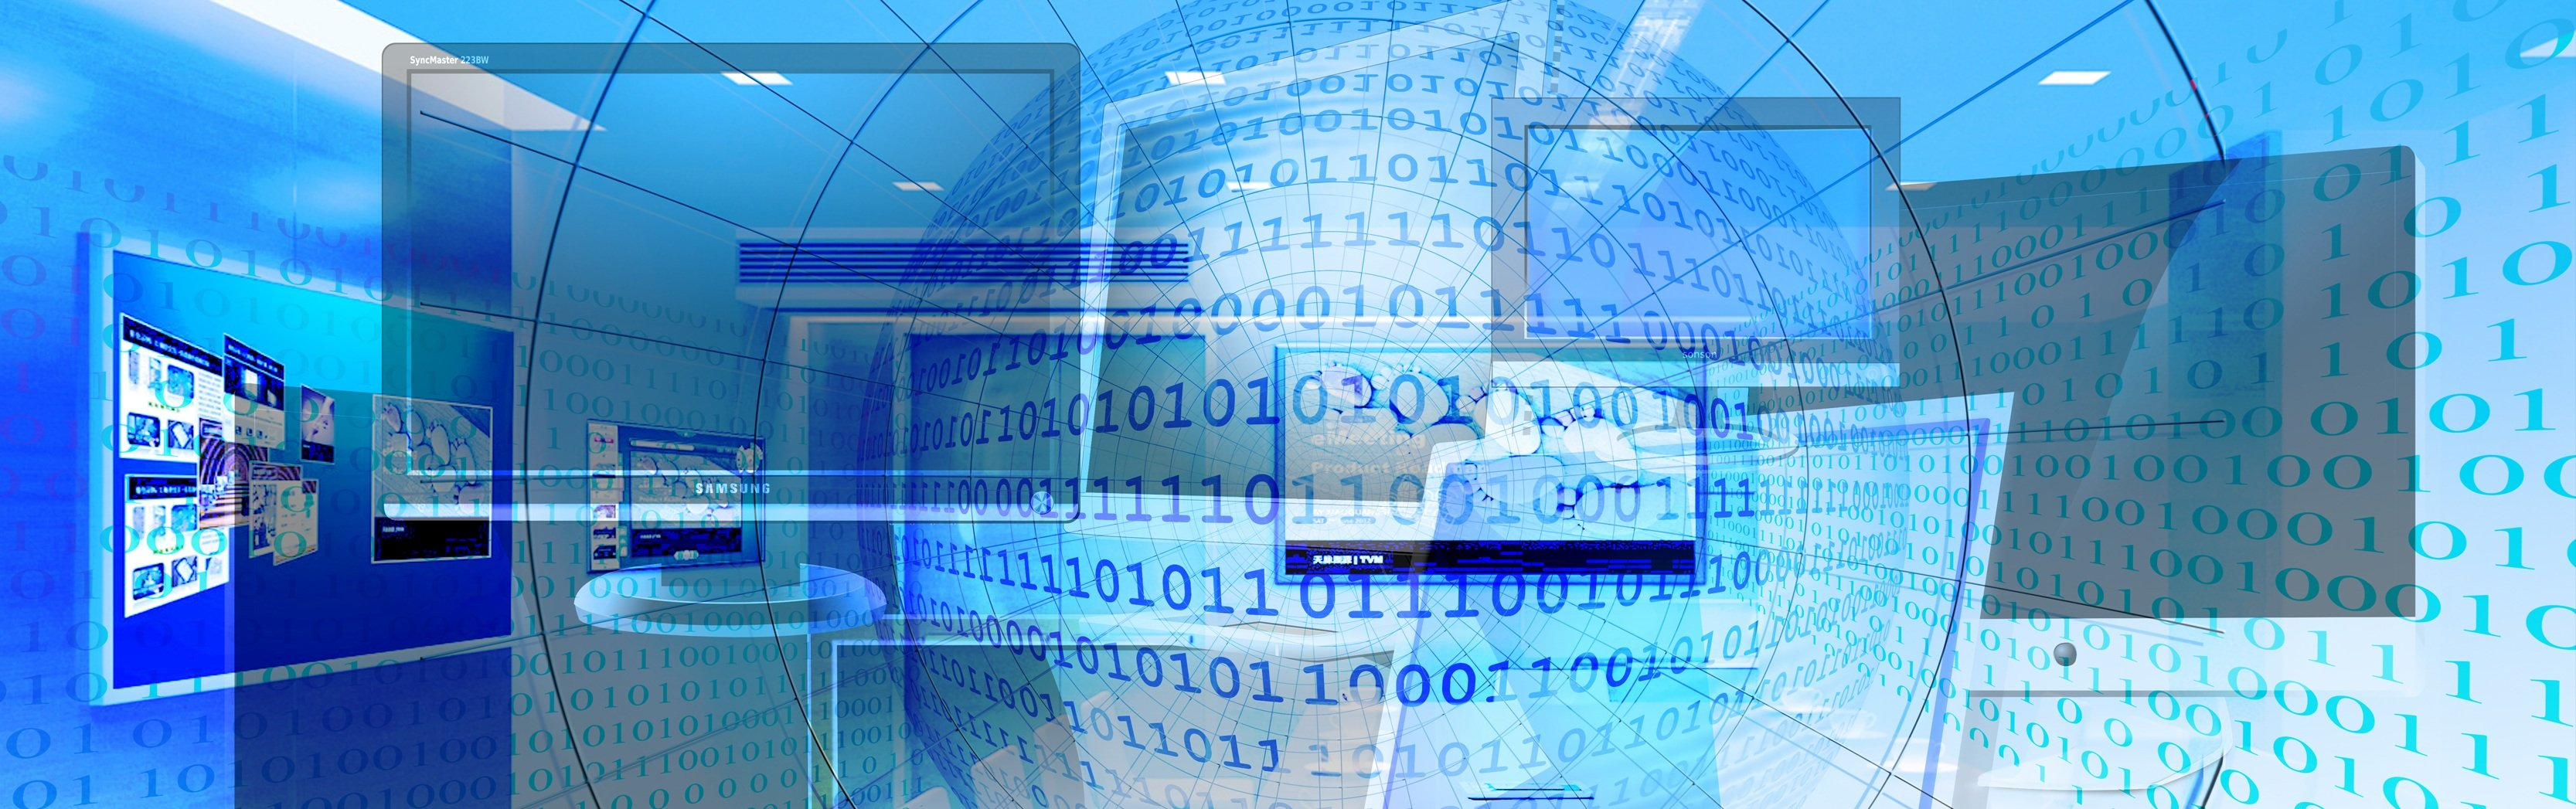
\includegraphics[width=\linewidth]{./Images/Chapter09/banner-pixabay-909710.jpg}
\end{jazzgraphic*}

\overparagraph{Ce que dit le programme}

\begin{tcolorbox}[title={Introduction}, toprule=0pt, leftrule=0pt, rightrule=0pt, arc=0pt,
                  fonttitle=\scshape\boxtitlefont,
                  colbacktitle=white, coltitle=firstcolor, colframe=firstcolor, colback=firstcolor!10,
                  breakable, enhanced jigsaw]
L’enseignement de sciences numériques et technologie en classe de seconde a pour objet de permettre d’appréhender les principaux concepts des sciences numériques, mais également de permettre aux élèves, à partir d’un objet technologique, de \emph{comprendre le poids croissant du numérique et les enjeux qui en découlent}.
L’enseignement de sciences numériques et technologie aide à mieux comprendre les enjeux scientifiques et sociétaux de la science informatique et de ses applications, à \emph{adopter un usage réfléchi et raisonné des technologies numériques} dans la vie quotidienne et à se préparer aux mutations présentes et à venir de tous les métiers.
Cet enseignement a vocation à multiplier les occasions de mise en activité des élèves, sous des formes variées (exposés, travaux en groupe, mini-projets, productions individuelles ou collectives, etc.) qui permettent de développer des compétences transversales [... comme] faire un \emph{usage responsable et critique} des sciences et technologies numériques.
\end{tcolorbox}

\begin{tcolorbox}[title={Impacts sur les pratiques humaines}, toprule=0pt, leftrule=0pt, rightrule=0pt, arc=0pt,
                  fonttitle=\scshape\boxtitlefont,
                  colbacktitle=white, coltitle=firstcolor, colframe=firstcolor, colback=firstcolor!10,
                  breakable, enhanced jigsaw]
L’évolution des capacités de stockage, de traitement et de diffusion des données fait qu’on assiste aujourd’hui à un phénomène de surabondance des données et au développement de nouveaux algorithmes capables de les exploiter.

Les centres de données (\textit{data center}) stockent des serveurs mettant à disposition les données et des applications les exploitant. \emph{Leur fonctionnement nécessite des ressources} (en eau pour le refroidissement des machines, en électricité pour leur fonctionnement, en métaux et en eau pour leur fabrication) et \emph{génère de la pollution} (manipulation de substances dangereuses lors de la fabrication, de la destruction ou du recyclage). De ce fait les \emph{usages numériques doivent être pensés de façon à limiter la transformation des écosystèmes} (notamment le réchauffement climatique) et à protéger la santé humaine.
\end{tcolorbox}

\subsubsection[Numérique : menace ou espoir pour l’environnement ?]{Numérique : menace ou espoir pour l’environnement ?}
\label{subsub:IX.4.1.2}

\noindent \href{https://ecoinfo.cnrs.fr/les-membres/francoise-berthoud-2/}{Françoise Berthoud},\caution[t]<firstcolor>{\href{https://ecoinfo.cnrs.fr/les-membres/francoise-berthoud-2/}{Françoise Berthoud}, ingénieure de recherche en informatique au \textsc{Cnrs} et cofondatrice du groupe \href{https://ecoinfo.cnrs.fr/}{EcoInfo} qu'elle dirige (créé en 2006), exerce une expertise reconnue sur la thématique des impacts environnementaux du numérique.}{À propos de l'intervenante} 
 conférences\parnote{Le diaporama est téléchargeable : \webdoc[\faFilePdfO/\faExternalLink]{https://www.fun-mooc.fr/asset-v1:inria+41018+session01+type@asset+block/Le_nume_rique_-_menace_ou_espoir_pour_l_environnement-inria_28_juin_2018_finale.pdf}{Numérique \textit{versus} environnement}.} Comprendre et Agir, \textsc{Inria}, juin 2018.
\parnotes

\vspace{6pt}

\begin{tcolorbox}[title={Résumé de l'intervention}, toprule=0pt, leftrule=0pt, rightrule=0pt, arc=0pt,
                  fonttitle=\scshape\boxtitlefont,
                  colbacktitle=white, coltitle=fourthcolor, colframe=fourthcolor, colback=fourthcolor!10,
                  breakable, enhanced jigsaw]
Envisagé comme solution technologique à la transition énergétique et plus globalement aux questions environnementales, le numérique est largement promu depuis plus de dix ans, par les sphères politiques, industrielles, voire par les citoyens et les chercheurs eux-mêmes. 

Quels effets aujourd’hui sur l’environnement pour quels impacts environnementaux ? Ne serait-il pas temps d’ouvrir les yeux sur une réalité qui a dépassé nos fantasmes collectifs ?
\end{tcolorbox}

\begin{marginvideo}
	[\label{vid:IX.9}Numérique \textup{versus} environnement.]%
	\movie[width=\marginparwidth,showcontrols]%
		{
\includegraphics[width=\marginparwidth]{./Images/Pictograms/film-strip-dark-electric-blue.png}}%
		{./Videos/Chapter09/vidIX-09-conf-digital-francoise-berthoud.mp4}%
	\launchvideo{./Videos/Chapter09/vidIX-09-conf-digital-francoise-berthoud.mp4}
\end{marginvideo}


\subsection[Impacts environnementaux]{Impacts environnementaux du numérique}
\label{sub:IX.4.2}

\subsubsection[Aspects de fabrication]{Aspects relatifs à la fabrication}
\label{subsub:IX.4.2.1}

\overparagraph{Des milliards d'appareils dans le monde}

\begin{jazzfigure}
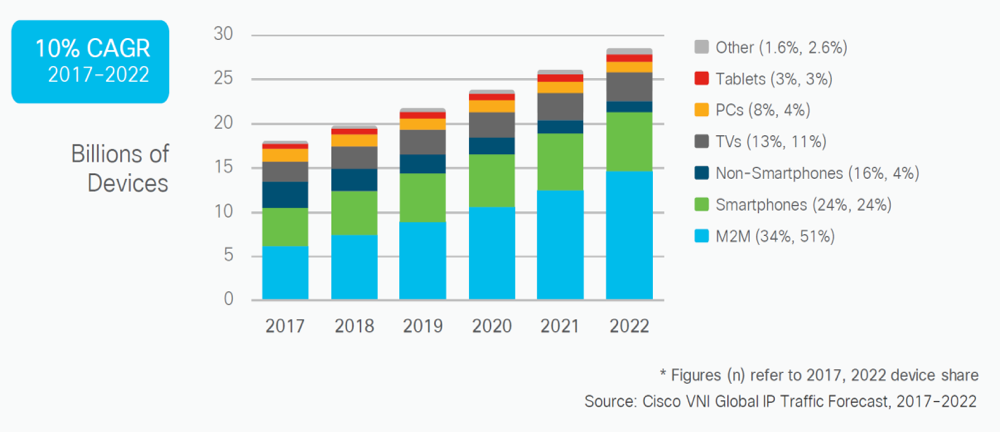
\includegraphics[width=\linewidth]{./Images/Chapter09/figIX-03-billions-of-devices.png}
\caption{\label{fig:IX.3}Évolution et prospectives des équipements numériques dans le monde.}
\end{jazzfigure}


\overparagraph{Utilisation de métaux rares --- or, argent, palladium...}

\begin{jazzitemize}
\item La fabrication\sidenote{L'article \pdfdoc[\faFilePdfO/\faExternalLink]{./Documents/Chapter09/docIX-02-marquet-etal-1024-sif-13-2019pdf}{Introduction aux impacts environnementaux du numérique} est disponible en consultation directe.} d’un \textit{smartphone} fait intervenir une cinquantaine de métaux [\href{https://www.societe-informatique-de-france.fr/wp-content/uploads/2019/04/1024-numero-13_Article19.pdf}{Introduction aux impacts environnementaux du numérique}, Kevin \textsc{Marquet}, Françoise \textsc{Berthoud}, Jacques \textsc{Combaz}, 1024 numéro 13, Avril 2019] (et plus généralement 70 matériaux différents).
\item « Au rythme actuel de production les réserves seraient de 15 ans pour l’étain, de 16 ans pour l’or, de 20 ans pour l’argent, ou encore de 39 ans pour le cuivre. Cependant, ces estimations doivent être prises avec précaution puisqu’elles ne tiennent compte que des réserves connues sans considérer les futures découvertes, les améliorations technologiques, ou les évolutions économiques ». [\href{https://www.societe-informatique-de-france.fr/wp-content/uploads/2019/04/1024-numero-13_Article19.pdf}{Introduction aux impacts environnementaux du numérique}, Kevin \textsc{Marquet}, Françoise \textsc{Berthoud}, Jacques \textsc{Combaz}, 1024 numéro 13, Avril 2019].
\item « Jusqu’à récemment, l’amélioration technologique a permis une augmentation continue de l’efficacité énergétique d’extraction (d’environ 1\,\% par an), et ce malgré la diminution en concentration du minerai de cuivre dans les exploitations. Du fait de limites physiques inhérentes aux processus d’extraction, cette tendance est en train de s’inverser et la quantité d’énergie nécessaire à l’extraction du cuivre devrait s’envoler d’ici la fin du siècle selon certains spécialistes » [O. Vidal, conférence dans le cycle « Comprendre et Agir », INRIA ,2019]. « Ce schéma s’applique à plus ou moins long terme à toutes les ressources minières, ce qui limitera tôt ou tard nos capacités d’extraction ». [\href{https://www.lemonde.fr/blog/binaire/2019/06/17/plus-d-ambitions-climatiques/}{Plus d’ambitions climatiques !} Françoise \textsc{Berthoud}, Jacques \textsc{Combaz} et Kevin \textsc{Marquet}, \textsc{Binaire}, 17 juin 2019].
\end{jazzitemize}

\begin{jazzfigure}
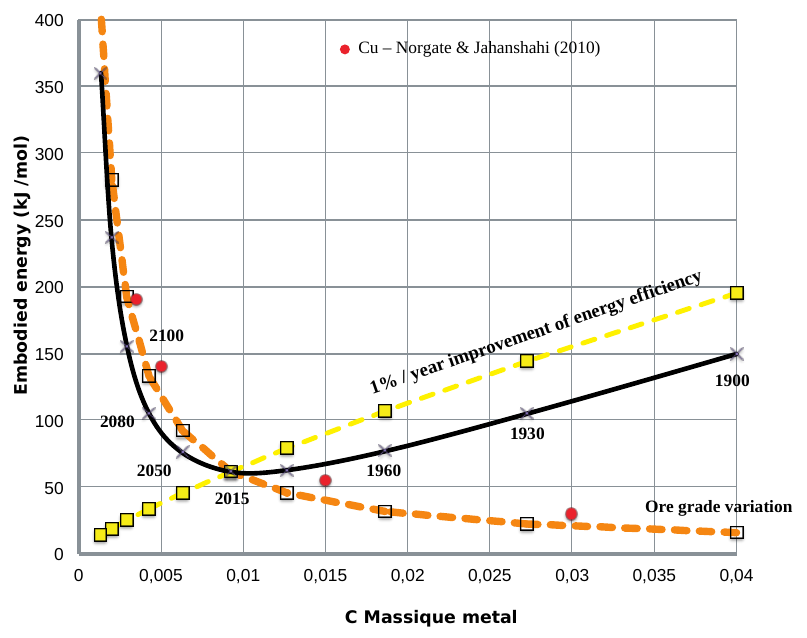
\includegraphics[width=\linewidth]{./Images/Chapter09/figIX-04-vidal-binaire-2019.png}
\caption{\label{fig:IX.4}Augmentation de l'énergie nécessaire à l’extraction du cuivre (d'après \textsc{Vidal}, conférence du cycle « Comprendre et Agir », \textsc{Inria}, 2019).}
\end{jazzfigure}

\begin{jazzfigure*}
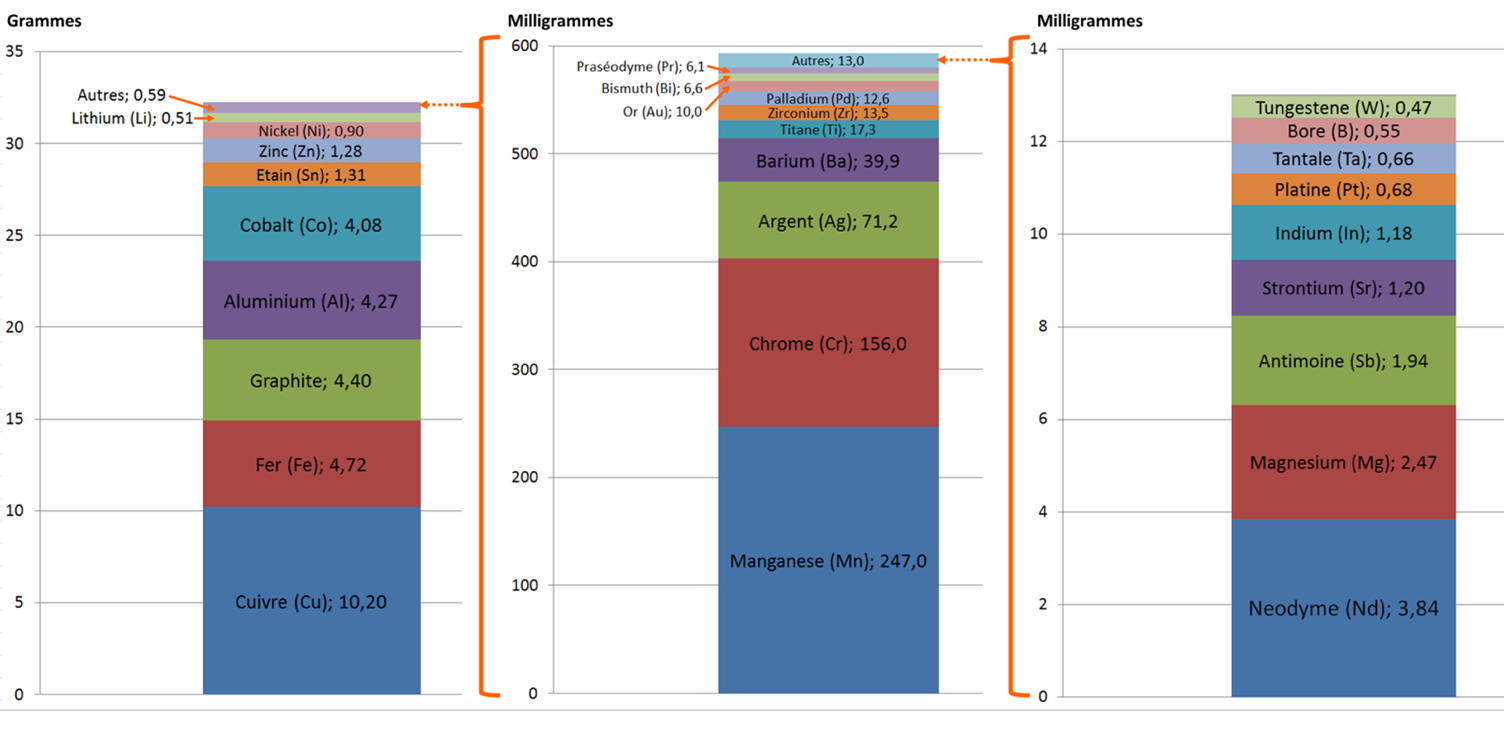
\includegraphics[width=\linewidth]{./Images/Chapter09/figIX-05-composition-smartphone-src-orange.png}
\caption{\label{fig:IX.5}Composition traditionnelle d’un \textup{smartphone} (source \textsc{Orange}).}
\end{jazzfigure*}


\overparagraph{Coûts énergétiques élevés de production}

« L’énergie est nécessaire non seulement pour le fonctionnement électrique des différents appareils électroniques (cf. \cref{fig:IX.3} terminaux : ordinateur personnel fixe et portable, tablette, \textit{smartphone}, téléphone portable traditionnel, box d’accès à internet, équipements audiovisuels connectés), mais aussi pour leur fabrication, leur transport et leur traitement en fin de vie »  \parencite{Marquet-et-al:2019}.

%[\href{https://www.societe-informatique-de-france.fr/wp-content/uploads/2019/04/1024-numero-13_Article19.pdf}{Introduction aux impacts environnementaux du numérique}, Kevin \textsc{Marquet}, Françoise \textsc{Berthoud}, Jacques \textsc{Combaz}, 1024 numéro 13, Avril 2019].

\begin{jazzfigure}
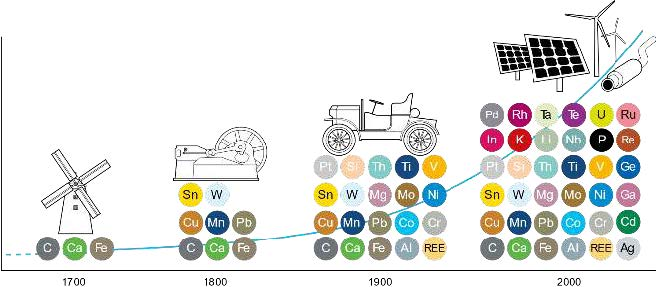
\includegraphics[width=\linewidth]{./Images/Chapter09/figIX-06-metals-tic-zepf-2014.jpg}
\caption{\label{fig:IX.6}Utilisation des métaux dans les TIC (d'après V. Zepf, 2014).}
\end{jazzfigure}

\begin{marginfigure}
\centering
%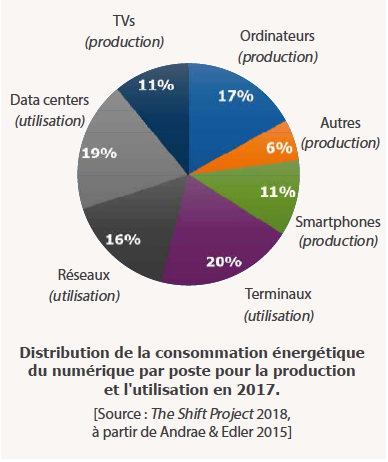
\includegraphics[width=\linewidth]{./Images/Chapter09/figIX-07-distribution-consommation.png}
\begin{tikzpicture}[scale=1, font=\scriptsize]
%\draw[step=0.25cm,style=help lines, line width=0.1pt] (-2.6,-2) grid (2.6,2);
%\draw[step=1cm,style=help lines, line width=0.8pt] (-2.5,-2) grid (2.5,2);
\pie[pos={-0.1,0}, radius=1.125, rotate=6]{%
6/{\fontsize{6.0pt}{0pt}\selectfont\begin{tabular}{@{}c@{}}Autres, \\(production)\end{tabular}},
17/{\fontsize{6.0pt}{0pt}\selectfont\begin{tabular}{@{}c@{}}Ordinateurs, \\(production)\end{tabular}}, 
11/{\fontsize{6.0pt}{0pt}\selectfont\begin{tabular}{@{}c@{}}TVs, \\(production)\end{tabular}},
19/{\fontsize{6.0pt}{0pt}\selectfont\begin{tabular}{@{}c@{}}Data centers, \\(utilisation)\end{tabular}},
16/{\fontsize{6.0pt}{0pt}\selectfont\begin{tabular}{@{}c@{}}Réseaux, \\(utilisation)\end{tabular}},
20/{\fontsize{6.0pt}{0pt}\selectfont\begin{tabular}{@{}c@{}}Terminaux, \\(utilisation)\end{tabular}},
11/{\fontsize{6.0pt}{0pt}\selectfont\begin{tabular}{@{}c@{}}Smartphones, \\(production)\end{tabular}}}
\end{tikzpicture}
\caption{\label{fig:IX.7}Distribution de la consommation énergétique du numérique par poste en 2017 (d'après \textup{The Shift Project}, 2018 --- à partir de \textsc{Andrae} \& \textsc{Edler} 2015).}
\end{marginfigure} %pour la production et l'utilisation

%\begin{jazzfigure}
%\begin{tikzpicture}[scale=1, font=\footnotesize]
%\piechart{%
%6/{\tiny\begin{tabular}{@{}c@{}}Autres, \\(production)\end{tabular}}/red,
%17/{\tiny\begin{tabular}{@{}c@{}}Ordinateurs, \\(production)\end{tabular}}/blue, 
%11/{\tiny\begin{tabular}{@{}c@{}}TVs, \\(production)\end{tabular}}/red,
%19/{\tiny\begin{tabular}{@{}c@{}}Data centers, \\(utilisation)\end{tabular}}/green,
%16/{\tiny\begin{tabular}{@{}c@{}}Réseaux, \\(utilisation)\end{tabular}}/yellow,
%20/{\tiny\begin{tabular}{@{}c@{}}Terminaux, \\(utilisation)\end{tabular}}/cyan,
%11/{\tiny\begin{tabular}{@{}c@{}}Smartphones, \\(production)\end{tabular}}/gray}
%\end{tikzpicture}
%\caption{\label{fig:IX.8}Test.}
%\end{jazzfigure}

\vspace{6pt}

On voit en \cref{fig:IX.7} que pour l'ensemble des appareils électroniques pris en compte, la phase de production correspond à 45\,\% de l'énergie totale utilisée durant le cycle de vie de ces appareils.

« Contrairement à une croyance bien installée, l’énergie consommée pendant la phase d’usage des équipements n’est pas prédominante. Le tableau [\ref{tab:IX.4}] donne le ratio du coût énergétique de la phase d’utilisation par rapport à la phase de production de divers appareils ». À noter que l'usage d'Internet est absent de ces estimations. Par exemple, en France, la phase d'usage d'un \textit{smartphone} n'est responsable que de 0,3\,\% des émissions de GES sur tout son cycle de vie (cf. \cref{fig:IX.8}) \parencite{Marquet-et-al:2019}. 

%[\href{https://www.societe-informatique-de-france.fr/wp-content/uploads/2019/04/1024-numero-13_Article19.pdf}{Introduction aux impacts environnementaux du numérique}, Kevin \textsc{Marquet}, Françoise \textsc{Berthoud}, Jacques \textsc{Combaz}, 1024 numéro 13, Avril 2019].

\vspace{8pt}

\begin{jazztable}
\caption{\label{tab:IX.4}Énergie consommée et gaz à effet de serre (GES) induits par les phases de production et d'usages de quelques équipements. }
\Centering
\begingroup
\small
\renewcommand*{\arraystretch}{1.6}
\rowcolors{2}{tableLineOne}{tableLineTwo}
\begin{tabularx}{\linewidth}{Xrrrrr}
\rowcolor{secondcolor}
\multicolumn{6}{c}{\Gape[6pt]{\textcolor{white}{\textbf{Énergie consommée des équipements numériques}}}} \\
\rowcolor{firstcolor}
\makecell{\scshape\titlingfont\textcolor{white}{Ratio}}
	& &	\multicolumn{4}{c}{\scshape\titlingfont\textcolor{white}{En émissions de GES}} \\
\rowcolor{firstcolor}
  %\multirowcell{-1}{\scshape\titlingfont\textcolor{white}{Ratio usage/production}}
  \makecell{\scshape\titlingfont\textcolor{white}{usage/production}}
  & \multirowcell{-2}{\scshape\titlingfont\textcolor{white}{En énergie}} 
  & \textsc{\titlingfont\textcolor{white}{France}}
  & \textsc{\titlingfont\textcolor{white}{Europe}}
  & \textsc{\titlingfont\textcolor{white}{USA}}
  & \textsc{\titlingfont\textcolor{white}{Chine}} \\
\textit{Smartphone} (2 ans)
  & 6\,\% & 0,3\,\% & 2,6\,\% & 4,5\,\% & 6,2\,\% \\
\textit{Laptop} (3 ans)
  & 11\,\% & 0,4\,\% & 2,9\,\% & 5,1\,\% & 6,9\,\% \\
Serveur
  & --- & 50\,\% & --- & --- & --- \\
TV connectée
  & --- & 1,1\,\% & 8,9\,\% & 15,0\,\% & 19,5\,\% \\
\end{tabularx}%
\endgroup
\end{jazztable}


\begin{jazzfigure*}
\Centering
\begin{tikzpicture}[scale=1, font=\footnotesize]
%\draw[step=0.25cm,style=help lines, line width=0.1pt] (0,-3.25) grid (16.5,2);
%\draw[step=1cm,style=help lines, line width=0.8pt] (0,-3.25) grid (16.5,2);
\node (S) at (2.75,0.5) {
\includegraphics[scale=0.4]{figIX-08-00-smartphone.pdf}};
\node[below=2pt of S, align=center, font=\footnotesize\lightboldfont, fill=secondcolor, text=white] (cartouche) 
  {\textit{Smartphone} gardé deux ans :\\ 90\,\% de consommation en énergie\\ avant l'achat (hors réseaux et \textit{data centers})};
\node[inner sep=0pt] (extraction) at (5.5,1) {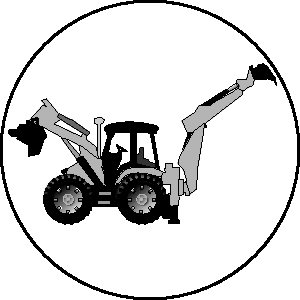
\includegraphics[width=2cm]{figIX-08a-extraction.pdf}};
\node[inner sep=0pt] (manufacturing) at (8,1) {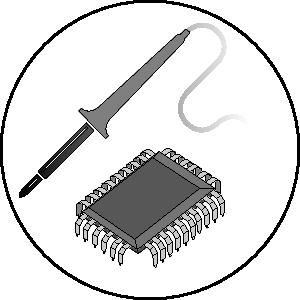
\includegraphics[width=2cm]{figIX-08b-manufacturing.pdf}};
\node[inner sep=0pt] (transport) at (10.5,1) {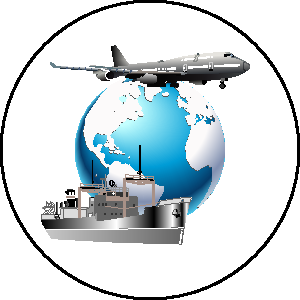
\includegraphics[width=2cm]{figIX-08c-transport.pdf}};
\node[inner sep=0pt] (use) at (13,1) {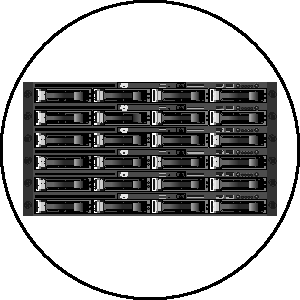
\includegraphics[width=2cm]{figIX-08d-use.pdf}};
\node[inner sep=0pt] (recycle) at (15.5,1) {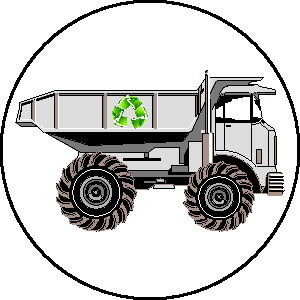
\includegraphics[width=2cm]{figIX-08e-recycle.pdf}};
%---
\node[inner sep=0pt, anchor=north east, font=\scriptsize] at ([xshift=-2.0mm, yshift=-0.5mm]extraction.south) {Extraction};
\node[inner sep=0pt, anchor=north east, font=\scriptsize] at ([xshift=-2.0mm, yshift=-0.5mm]manufacturing.south) {Fabrication};
\node[inner sep=0pt, anchor=north east, font=\scriptsize] at ([xshift=-2.0mm, yshift=-0.5mm]transport.south) {Transport};
\node[inner sep=0pt, anchor=north east, font=\scriptsize] at ([xshift=-2.0mm, yshift=-0.5mm]use.south) {Utilisation};
\node[inner sep=0pt, anchor=north east, font=\scriptsize] at ([xshift=-2.0mm, yshift=-0.5mm]recycle.south) {Recyclage};
%---
\draw[secondcolor, line width=1.6pt] (extraction.south) 
  -- ([yshift=-5mm]extraction.south) -- ([yshift=-5mm]manufacturing.south);
\draw[secondcolor, line width=1.6pt] (manufacturing.south) 
  -- ([yshift=-5mm]manufacturing.south) -- ([yshift=-5mm]transport.south);
\draw[firstcolor, line width=1.6pt] (transport.south) 
  -- ([yshift=-5mm]transport.south) -- ([yshift=-5mm]use.south);
\draw[firstcolor, line width=1.6pt] (use.south) 
  -- ([yshift=-5mm]use.south) -- ([yshift=-5mm]recycle.south);
\draw[firstcolor, line width=1.6pt] (recycle.south) -- ([yshift=-5mm]recycle.south);
%---
\draw[-latex, secondcolor, line width=1.6pt] (7.0,-0.5) -- (7.0,-1.25) -- (8.5,-1.25);
\draw[-latex, firstcolor, line width=1.6pt] (14.0,-0.5) -- (14.0,-1.25) -- (12.5,-1.25);
\node[inner sep=0pt, font=\scriptsize, align=center] at (10.5,-1.25) 
  {Consommation d'électricité\\ (10\,\% niveau mondial)};
\draw[-latex, secondcolor, line width=1.6pt] (7.5,-1.25) -- (7.5,-2.0) -- (8.5,-2.0);
\draw[-latex, firstcolor, line width=1.6pt] (13.5,-1.25) -- (13.5,-2.0) -- (12.5,-2.0);
\node[inner sep=0pt, font=\scriptsize, align=center] at (10.5,-2.0) 
  {Consommation d'énergie primaire\\ (4\,\% niveau mondial, +8\,\%/an)};
\draw[-latex, secondcolor, line width=1.6pt] (8.0,-2.0) -- (8.0,-2.75) -- (8.5,-2.75);
\draw[-latex, firstcolor, line width=1.6pt] (13.0,-2.0) -- (13.0,-2.75) -- (12.5,-2.75);
\node[inner sep=0pt, font=\scriptsize, align=center] at (10.5,-2.75) {Changement climatique};
\node[inner sep=0pt, font=\footnotesize, anchor=south west, text=secondcolor] at (7.25,-1.0) {\lightbf{90\,\%}};
\node[inner sep=0pt, font=\footnotesize, anchor=south east, text=firstcolor] at (13.75,-1.0) {\lightbf{10\,\%}};
%---
\node[inner sep=0pt] at (6.5,-1.25) {
\includegraphics[scale=0.6]{figIX-08-01-electric-arc.pdf}};
\node[inner sep=0pt] at (15.25,-1.75) {
\includegraphics[scale=0.4]{figIX-08-02-oil-pump.pdf}};
%\node[inner sep=0pt] at (13.5,-2.75) {
\includegraphics[scale=0.25]{figIX-08-03-thermometer.pdf}};
\node[inner sep=0pt] at (7.5,-2.75) {
\includegraphics[scale=0.2]{figIX-08-03-thermometer.pdf}};
\end{tikzpicture}
\caption{\label{fig:IX.8}Impact environnemental des TIC : énergie des \textup{smartphones} (d'après \href{./Documents/Chapter09/combaz-berthoud-2019-02-18-polytech.pdf}{Jacques \textsc{Combaz} et Françoise \textsc{Berthoud}}, 2019).}
\vspace{-4pt}
\end{jazzfigure*}


\subsubsection[Aspects de consommation]{Aspects relatifs à la consommation}
\label{subsub:IX.4.2.2}

\overparagraph{Consommation énergétique relative au numérique}

« Aujourd’hui, les Technologies de l’information et de la communication (TIC) (équipements terminaux dont téléviseurs, équipements réseau, serveurs et leur environnement) sont responsables d’au moins 10 \,\% de la consommation électrique mondiale, si l’on considère les phases de production et d’usage ». [\href{https://theshiftproject.org/lean-ict/}{Lean ict : Pour une sobriété numérique}. Technical report, \textit{The Shift Project}, 2018].

\vspace{6pt}
\begin{jazzfigure}
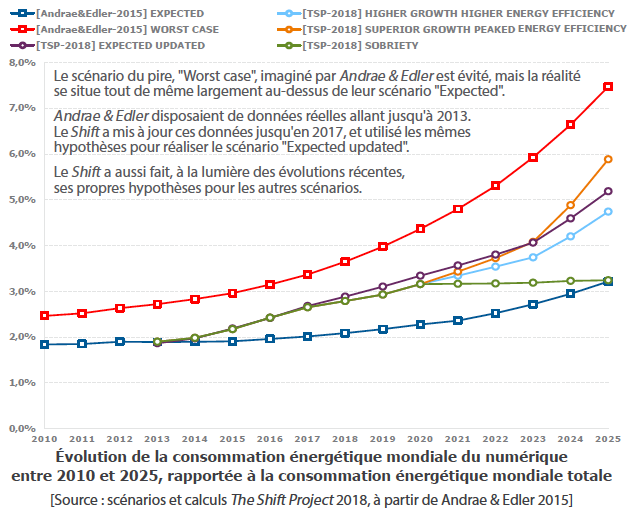
\includegraphics[width=\linewidth]{figIX-09-evolution-consommation.png}
\caption{\label{fig:IX.9}Évolution de la consommation énergétique mondiale du numérique rapportée à la con\-sommation énergétique totale (d'après The Shift Project, 2018 -- à partir de \textsc{Andrae} \& \textsc{Edler} 2015).}
\end{jazzfigure}

\vspace{6pt}
\begin{jazzfigure}
\centering
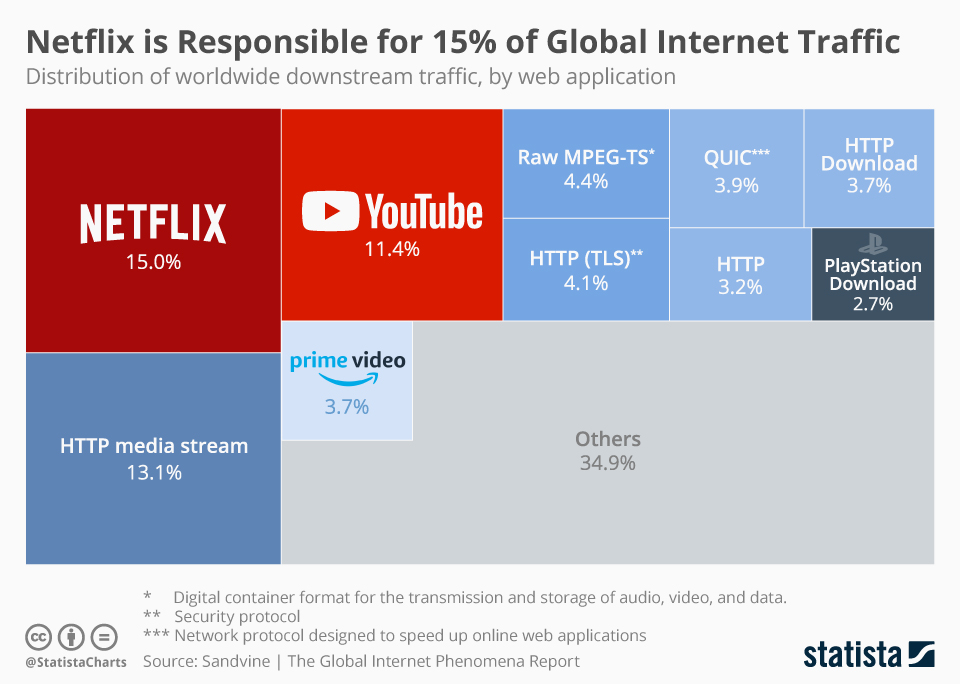
\includegraphics[width=0.95\linewidth]{figIX-10-global-downstream-traffic-2018.jpg}
\caption{\label{fig:IX.10}Distribution au niveau mondial du trafic de téléchargement (chiffres octobre 2018).}
\end{jazzfigure}


%\overparagraph{Streaming vidéo et production de \texorpdfstring{CO$_2$}{CO\texttwoinferior}}
\overparagraph{Streaming vidéo et production de CO\texorpdfstring{\textsubscript{2}}{\texttwoinferior}}

« L'association \textit{The Shift Project} a fait ses calculs, rendus publics la semaine dernière : l'usage des \textsc{Netflix} et autres \textsc{YouTube} a produit 306 millions de tonnes de CO\textsubscript{2} en 2018. Autant que l'Espagne.

Dans le détail, la consommation de vidéos dites “\textit{online}”, hébergées sur un serveur et transmises sur un terminal (\textit{smartphone}, TV…) distant \textit{via} un réseau, est à l’origine de 60\,\% du trafic de données numériques dans le monde l’an dernier. Inclus dans cette catégorie, les services à la \textsc{Netflix} et à la \textsc{Amazon Prime} comptent pour 34\,\% de ce total, suivis par les portails pornographiques (27\,\%), les plateformes telles que \textsc{YouTube} et \textsc{DailyMotion} (21\,\%) et enfin les vidéos partagées sur les réseaux sociaux (18\,\%) ».

\noindent Source : \href{https://www.techniques-ingenieur.fr/actualite/articles/le-streaming-video-une-usine-a-co2-68488/}{Le streaming vidéo, une usine à CO\textsubscript{2}}, Frédéric \textsc{Monflier}, Informatique et Numérique, juillet 2019.



\overparagraph{Consommation énergétique des centres de données}

En \cref{fig:IX.11}, une « ferme de serveurs » de \textsc{Facebook} aux États-Unis. Un gros \textit{data center} consomme 100 millions de watts (100 MW), soit un dixième de la production d’une centrale thermique. [Source : \href{https://lejournal.cnrs.fr/articles/numerique-le-grand-gachis-energetique}{Le grand gâchis énergétique}, 2018, Laure \textsc{Cailloce}, \textsc{Cnrs Le journal}].


\begin{marginfigure}
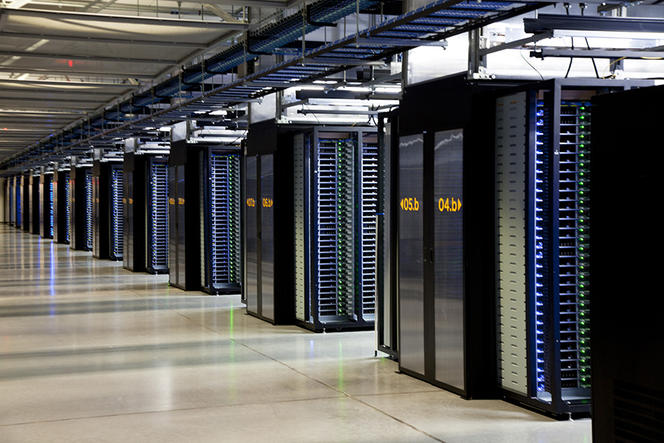
\includegraphics[width=\linewidth]{figIX-11-facebook-datacenter-kim-steele-gettyimages-72dpi.jpg}
\caption{\label{fig:IX.11}Data center \textsc{Facebook}.}
\end{marginfigure}

%\sidegraphic[\label{fig:IX.11}Data center \textsc{Facebook}.]{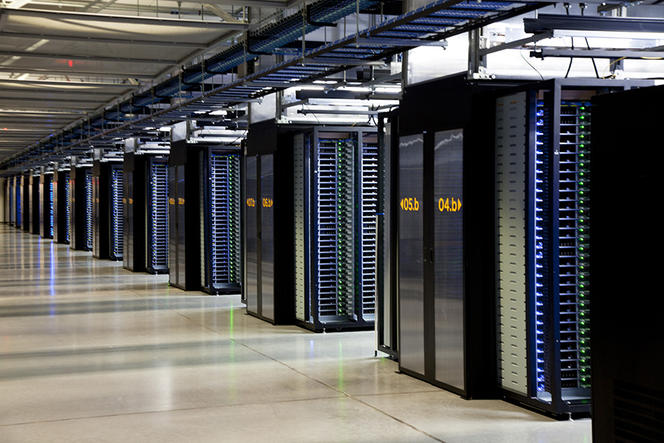
\includegraphics[width=\linewidth]{figIX-11-facebook-datacenter-kim-steele-gettyimages-72dpi.jpg}}{Kim Steele -- Getty images}

« Les \textit{data centers}, ces usines de la donnée qui abritent des milliers de serveurs informatiques, sont-ils des gouffres énergétiques ? Le numérique, qui a pris une place inédite dans nos vies, a lui aussi une empreinte écologique. Dans son ensemble, le secteur du numérique engloutissait près de 10\,\% de la production électrique mondiale en 2015. Les \textit{data centers} en accaparent 18\,\%, selon une \href{http://decrypterlenergie.org/la-revolution-numerique-fera-t-elle-exploser-nos-consommations-denergie}{synthèse publiée fin 2017 par l'association \textsc{négaWatt}} et reprise par le site \textsc{GreenIT}. À quoi servent ces centres de données et que penser de leur consommation d'énergie ? La révolution numérique est passée par là, entraînant dans son sillage de nouvelles pratiques, dont celle du \textit{cloud computing} (ou "informatique dématérialisée"). D'ici 2021, la capacité de stockage des data centers devrait encore être multiplié par quatre, selon \href{https://www.cisco.com/c/en/us/solutions/executive-perspectives/annual-internet-report/index.html}{une étude de \textsc{Cisco}}. En fait, le stockage des données est dans ce cas externalisé par des sociétés spécialisées, qui se chargent de ses aspects opérationnels et matériels. De quoi faciliter l'administration des serveurs, en les confiant à des professionnels... Et surtout réduire les durées d'interruption lorsque des pannes se produisent. Le numérique pesant désormais lourdement dans l'économie, on comprend qu'un site de e-commerce (par exemple) souhaite réduire au plus bas la durée où ses pages sont inaccessibles ». [\href{https://www.sciencesetavenir.fr/high-tech/informatique/numerique-et-ecologie-les-data-centers-des-gouffres-energetiques_121838}{Numérique et écologie : les \textit{data centers}, des gouffres énergétiques ?}, Sarah \textsc{Sermondadaz}, \textsc{Sciences et avenir}, Mars 2018].


\paragraph{Récupérer la chaleur des \textit{data centers}}
« En France, la consommation des \textit{data centers} s'élevait à environ 3 TWh en 2015, soit davantage que la consommation électrique de la ville de Lyon, selon l'\href{https://ufe-electricite.fr/}{Union française de l'électricité} (UFE). À quoi tient-elle ? Il faut bien entendu alimenter en électricité les nombreux appareils. Mais elle est principalement dissipée sous forme de chaleur lorsqu'elle passe dans un matériau conducteur, ce qu'on appelle "effet Joule". De ce fait, environ 50\,\% de la facture d'électricité d'un data center... Tient à la climatisation, \href{https://www.actu-environnement.com/ae/dossiers/efficacite-energetique/data-centers-reduire-facture-energetique-rester-competitifs.php}{comme l'expliquaient nos confrères de \textsc{Actu-Environnement}}. Pour réduire leurs coûts, les \textit{data centers} ont alors tout intérêt à maximiser le “\textit{free cooling}”, ou refroidissement naturel en utilisant l'air frais extérieur. C'est pour cette raison que des géants comme \textsc{Facebook} (par exemple) ont \href{https://www.sciencesetavenir.fr/decryptage/pourquoi-les-centres-de-traitement-des-donnees-migrent-ils-au-nord_37030}{délocalisé leurs serveurs dans des pays nordiques comme la Suède} » [\href{https://www.sciencesetavenir.fr/high-tech/informatique/numerique-et-ecologie-les-data-centers-des-gouffres-energetiques_121838}{Numérique et écologie : les \textit{data centers}, des gouffres énergétiques ?}, Sarah \textsc{Sermondadaz}, \textsc{Sciences et avenir}, Mars 2018].

\paragraph{Des équipements surdimensionnés}
« Autre particularité du Web, son « hyperdisponibilité » : toutes les infrastructures sont dimensionnées pour absorber les afflux de données liés aux pics d’utilisation, soit quelques heures par jour à peine, et demeurent sous-utilisées le reste du temps... Cette « tyrannie » de l’utilisateur se retrouve jusque dans la conception des box Internet qui ne possèdent pas de bouton d’arrêt et fonctionnent jour et nuit. « Il faut une minute trente pour rallumer une box éteinte ; les fournisseurs d’accès estiment que c’est un temps beaucoup trop long pour les utilisateurs impatients que nous sommes devenus », explique Françoise \textsc{Berthoud}. Résultat : les box représentent à elles seules 1\,\% de la consommation électrique française ». [\href{https://lejournal.cnrs.fr/articles/numerique-le-grand-gachis-energetique}{Le grand gâchis énergétique}, 2018, L. \textsc{Cailloce}, \textsc{Cnrs Le journal}].

\overparagraph{Stockage et acheminement des données}

« Dans la phase d’usage, une grande part de la dépense énergétique est le fait du stockage et de l’acheminement des données, c’est-à-dire des datacentres et des réseaux, sachant que le trafic réseau est en augmentation de 26\,\% par an ce qui est considérable. Il faut savoir qu’aujourd’hui 80 à 90\,\% du volume de données qui circule sur les réseaux est induit par la vidéo ».

« Dix minutes de streaming vidéo haute définition équivaut à utiliser à pleine puissance pendant cinq minutes un four électrique de 2000 W. L’\textsc{Ademe} estimait en 2011 que l’envoi d’un courriel contenant une pièce jointe de 1 Mo provoquait en moyenne l’émission d’environ 20 g de GES, soit l’équivalent libéré par la combustion du carburant nécessaire à la réalisation de 200 mètres en voiture » \parencite{Marquet-et-al:2019}.

\overparagraph{Des « obésiciels » trop gourmands}

« La couche logicielle qui permet à tous ces équipements de fonctionner n’est guère plus optimisée. C’est le cas des applications pour \textit{smartphones} développées à la va-vite pour pouvoir être mises rapidement sur le marché, qui consomment d’autant plus d’énergie qu’elles sont toujours ouvertes ». « La plupart des gens ne savent pas qu’en moyenne, trente-cinq applis tournent en permanence sur leur téléphone, qu’ils les utilisent ou pas », signale la chercheuse. Résultat, les batteries se vident en moins d’une journée, quand il suffirait de les éteindre en activant le mode économie d’énergie pour gagner jusqu’à plusieurs jours d’autonomie ». [\href{https://lejournal.cnrs.fr/articles/numerique-le-grand-gachis-energetique}{Le grand gâchis énergétique}, 2018, Laure \textsc{Cailloce}, \textsc{Cnrs Le journal}].

\sidegraphic{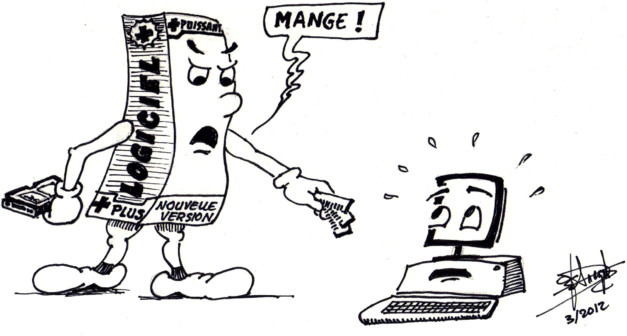
\includegraphics[width=\linewidth]{obesiciel-eric-drezet.png}}{Éric Drezet}%
« Cependant, toutes ces applications installées consomment des ressources de calcul et de stockage. Effectivement, même une application qui n’est jamais utilisée peut être programmée pour envoyer des notifications périodiques à des serveurs distants (des données de géolocalisation par exemple) et ainsi avoir une consommation énergétique non négligeable. Plusieurs techniques peuvent être mises en œuvre pour réduire l’impact des applications. Certaines relèvent de bonnes pratiques, notamment lorsqu’il s’agit d’être attentif et de personnaliser la configuration des applications. D’autres techniques s’inscrivent dans les domaines du génie logiciel et de l’éco-conception logicielle ». [\href{https://interstices.info/le-syndrome-de-lobesiciel-des-applications-energivores/}{Le syndrome de l’obésiciel : des applications énergivores}, Françoise \textsc{Berthoud}, Éric \textsc{Drezet}, Laurent \textsc{Lefèvre} et Anne-Cécile \textsc{Orgerie}, \textsc{Interstices}, juillet 2015].

\overparagraph{Pollutions diverses (eau, sol, air)}

\begin{jazzitemize}
\item Tarissement de l’eau.
\item Érosion des sols.
\item Fragmentation des territoires.
\end{jazzitemize}

\overparagraph{Efficience énergétique}

La loi de \textsc{Koomey} décrit une tendance à long terme dans l'histoire des ordinateurs. Selon cette loi, le nombre de calculs par joule d'énergie dépensé double tous les dix-huit mois environ. Il s'avère que cette tendance a été remarquablement stable depuis les années 1950, le nombre de calculs par joule d'énergie dépensé ayant doublé environ tous les 1,57 ans. Cette loi énoncée par Jonathan \textsc{Koomey} aurait été énoncée comme suit: la quantité d'énergie dont une machine a besoin pour effectuer un nombre donné de calculs va diminuer d'un facteur deux chaque année et demi [\href{https://fr.wikipedia.org/wiki/Loi_de_Koomey}{\faWikipediaW}].

\begin{marginfigure}
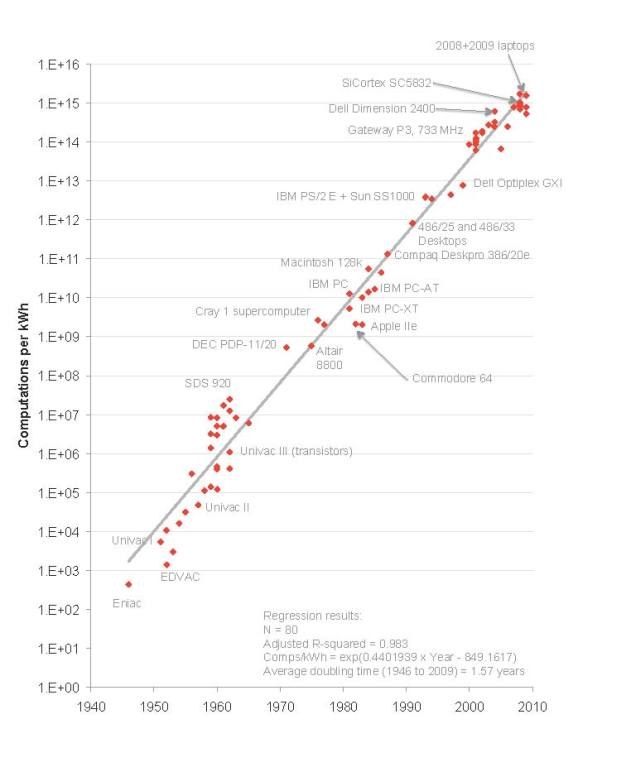
\includegraphics[width=\linewidth]{figIX-12-koomeys-law.jpg}
\caption{\label{fig:IX.12}Loi de Koney : nombre de calculs par kWh, de 1946 à 2009 (\href{https://fr.wikipedia.org/wiki/Loi_de_Koomey}{\normalfont\faWikipediaW}).}
\end{marginfigure}

\subsubsection[Aspects de recyclage]{Aspects relatifs au recyclage}
\label{subsub:IX.4.2.3}

\overparagraph{Traitement des déchets (DEEE)}

« Dans le monde, seulement 20\,\% (en poids) des déchets d’équipements électriques et  électroniques (DEEE) sont traités par des filières de recyclage identifiées. En France, ce taux est porté à 50\,\%. Aujourd’hui, la difficulté à réparer des appareils de plus en plus complexes mais aussi les diverses sources d’obsolescence nous incitent à un renouvellement toujours plus rapide de notre matériel électronique. Ainsi, un smartphone est remplacé après deux à deux années et demi en moyenne (88\,\% sont changés alors qu’ils fonctionnent encore), trois à cinq ans pour un ordinateur portable, cinq ans pour un ordinateur fixe~» \parencite{Marquet-et-al:2019}.

\overparagraph{Recyclage : espoir pour l'épuisement des ressources}

« Dans les composants électroniques, les métaux sont très peu recyclés ». [\href{https://lejournal.cnrs.fr/articles/numerique-le-grand-gachis-energetique}{Le grand gâchis énergétique}, 2018, L. \textsc{Cailloce}, \textsc{Cnrs Le journal}].

\begin{marginfigure}
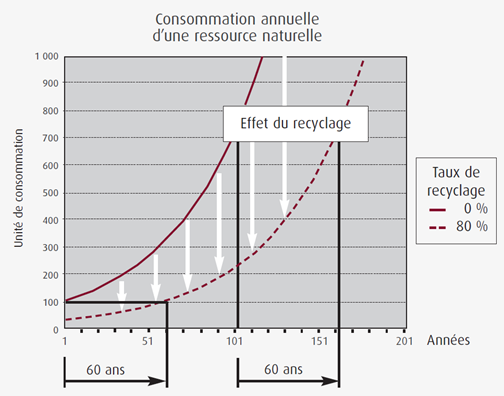
\includegraphics[width=\linewidth]{figIX-13-recyclage.png}
\caption{\label{fig:IX.13}Gain de temps permis par un fort taux de recyclage.}
\end{marginfigure}

« Le recyclage représente un espoir pour amortir l’épuisement des ressources, mais actuellement les taux de récupération des métaux dans les appareils électroniques sont faibles. Porter le recyclage à 80\,\% (et même à 100\,\% !) permettrait de retarder cet épuisement dans le contexte de demandes en croissance exponentielle observé actuellement, mais pas de s’inscrire dans un processus d’économie circulaire ». [\href{https://www.lemonde.fr/blog/binaire/2019/06/17/plus-d-ambitions-climatiques/}{Plus d’ambitions climatiques !} Françoise \textsc{Berthoud}, Jacques \textsc{Combaz} et Kevin \textsc{Marquet}, \textsc{Binaire}, 17 juin 2019].

\overparagraph{Obsolescence}

« La voracité en ressources matérielles des obésiciels contribue fortement à la chute de la durée moyenne d’utilisation des appareils électroniques (ordinateurs, smartphones, etc.) avant remplacement. En effet, ils ne sont pas capables de s’adapter à plusieurs générations successives de logiciels. C’est le phénomène de l’obsolescence : l’appareil est dépassé en raison de l’évolution des logiciels. »

\begin{jazzitemize}
\item Au niveau du matériel : lorsque les pièces détachées nécessaires à la réparation d’un appareil ne sont plus disponibles, l’appareil doit être remplacé en totalité.
\item Au niveau logiciel : incompatibilité de deux versions d’un logiciel, fin du support (par exemple, fin du support de \textsc{Windows XP} depuis 2014 qui devient vulnérable aux failles de sécurité).
\end{jazzitemize}

\noindent Source : \href{https://interstices.info/le-syndrome-de-lobesiciel-des-applications-energivores/}{Le syndrome de l’obésiciel : des applications énergivores}, Françoise \textsc{Berthoud}, Éric \textsc{Drezet}, Laurent \textsc{Lefèvre} et Anne-Cécile \textsc{Orgerie}, \textsc{Interstices}, Juillet 2015.

\subsubsection[Autre impacts]{Autre impacts}
\label{subsub:IX.4.2.4}

\overparagraph{Impacts sociopolitiques}

L'extraction des métaux nécessaires à la fabrication des équipements numériques est à l'origine de :
\begin{itemize}
\item conflits armés en République Démocratique du Congo ;
\item conflits sociaux liés à l'accès à l'eau et à la pollution en Amérique du Sud ;
\item conflits miniers en Amérique latine.
\end{itemize}

\overparagraph{Grandes inégalités d’accès aux services numériques}

Il faut également avoir à l'esprit que l'accès aux services numériques à travers le monde est très inégal. Les cartes en \cref{fig:IX.14} présente les proportions de population ayant accès à l'Internet dans les différentes parties du globe en 2017 (voir également \cref{fig:IX.2} pour 2016). Les écarts sont criants pour l'Afrique et une partie de l'Asie. % du Sud-Est.

%\vspace{6pt}
%\begin{jazzfigure*}
%\Centering
%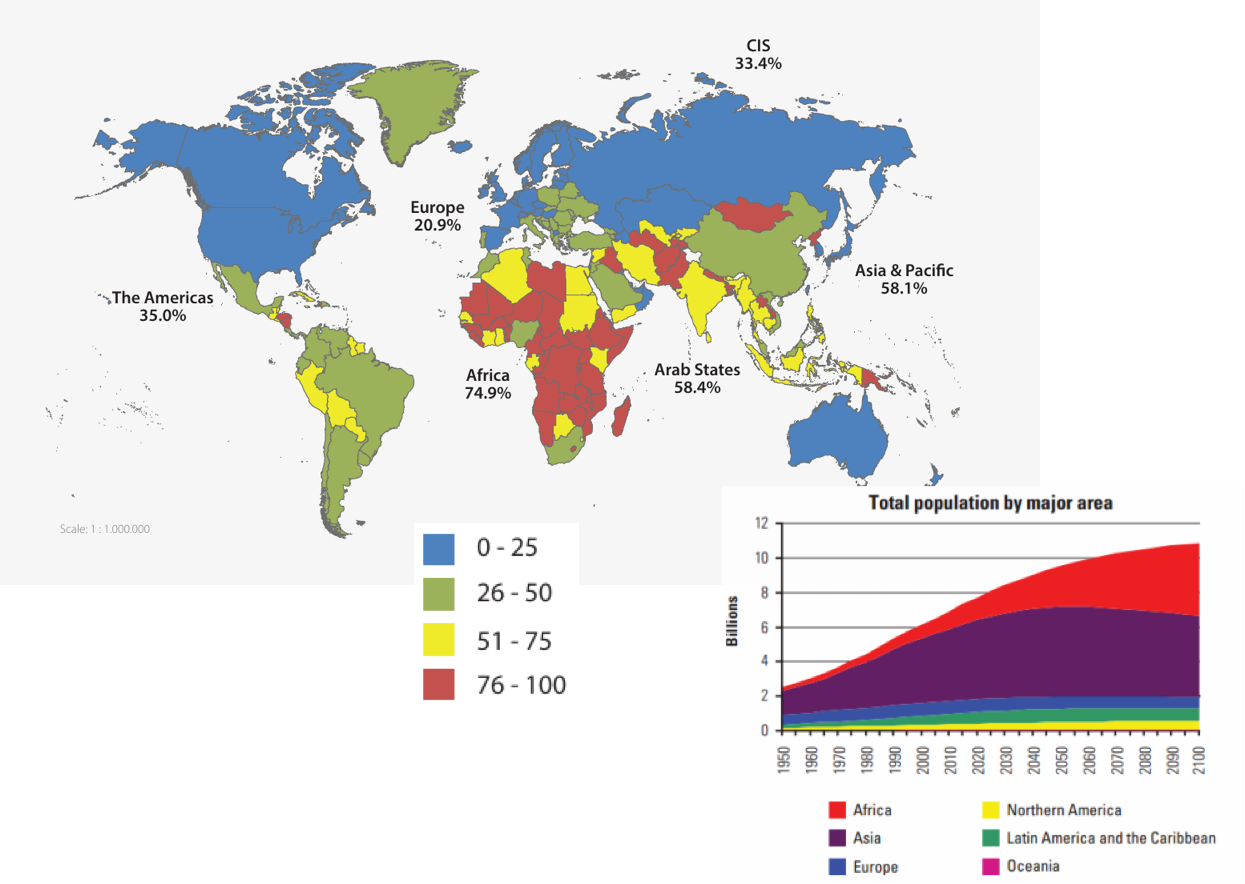
\includegraphics[width=\linewidth]{figIX-14-acces-internet-2016.png}
%\caption{\label{fig:IX.14}Évaluation par pays de l'accès à Internet des populations en 2017 (source \href{https://www.itu.int/fr/Pages/default.aspx}{ITU} et \href{https://ourworldindata.org/internet}{Our World in Data}).}
%\end{jazzfigure*}

\begin{jazzfigure*}
\begin{subfigure}{\linewidth}
\Centering
\includegraphics[width=\linewidth]{figIX-14a-number-of-internet-users-by-country-2017.pdf}
\caption{\label{figIX.14a}Nombre d'utilisateurs de l'Internet par pays.}
\end{subfigure}\\[6pt]
\begin{subfigure}{\linewidth}
\Centering
\includegraphics[width=\linewidth]{figIX-14b-share-of-individuals-using-the-internet-2017.pdf}
\caption{\label{figIX.14b}Part de la population utilisant l'Internet par pays.}
\end{subfigure}
\caption{\label{fig:IX.14}Évaluation par pays de l'accès à Internet des populations en 2017 --- les utilisateurs d'Internet sont les individus y ayant eu accès dans les trois derniers mois, tout équipement confondu (source \href{https://www.itu.int/fr/Pages/default.aspx}{ITU} et \href{https://ourworldindata.org/internet}{Our World in Data}).}
\vspace{-4pt}
\end{jazzfigure*}

\overparagraph{Impacts sur la santé}

Il faut noter également que l'usage du numérique a des impacts sur la santé, par exemple :
\begin{itemize}
\item addiction aux usages ;
\item troubles musculo-squelettiques...
\end{itemize}


\subsubsection[Comment agir ?]{Comment individuellement agir ?}
\label{subsub:IX.4.2.5}

« \emph{Choisir entre l’utile et le moins utile} : l’auto-régulation des fournisseurs de services et le volontarisme des usagers ne suffiront pas : l’association “\textit{The Shift Project}” plaide pour la mise en œuvre d’une régulation, à l’issue d’un débat sociétal, qui permet d’arbitrer entre ce qui est utile et ce qui l’est moins. 
\begin{margingraphic}
\includegraphics[width=\linewidth]{recycling-earth.pdf}
\end{margingraphic}
« Il ne s’agit pas d’être pour ou contre la pornographie, la télémédecine, \textsc{Netflix} ou les mails : il s’agit d’éviter qu’un usage précieux ne pâtisse de la surconsommation d’un autre jugé moins essentiel » expliquent les auteurs de l’étude. Cette démarche n’irait pas à l’encontre du principe de neutralité du net, pour lequel la nature des contenus prime sur leur volume ». [\href{https://www.techniques-ingenieur.fr/actualite/articles/le-streaming-video-une-usine-a-co2-68488/}{Le streaming vidéo, une usine à CO\textsubscript{2}}, F. \textsc{Monflier}, Informatique et Numérique, juillet 2019].


« L’allongement de la durée de vie des équipements est une des principales préconisations pour diminuer les impacts environnementaux des TIC » \parencite{Marquet-et-al:2019}.

On peut ainsi se tourner vers les « \textit{low tech} » à l'opposé de « \textit{high tech} ». « Le \textit{low-tech} ou basse technologie est un ensemble de techniques simples, pratiques, économiques et populaires. Elles peuvent faire appel au recyclage de machines récemment tombées en désuétude. Ce sont des solutions techniques qui cherchent à être simples, bien pensées, dimensionnées et réparables. Elles sont issues d'une fabrication locale, favorisant l'emploi, plus proche de l'artisanat que de la production industrielle, voire de la prosommation » [\href{https://fr.wikipedia.org/wiki/Low-tech}{\faWikipediaW}] (cf. \href{https://www.lowtechmagazine.com/}{\textsc{Low Tech Magazine}} pour plus d'informations sur le sujet).

\begin{jazzgraphic*}
\Centering
\includegraphics[width=\linewidth]{digital-thinking-banner-gerd-altmann-pixabay.jpg}
\end{jazzgraphic*}

« Afin d'éviter de saturer les serveurs distants : supprimer ses vieux courriels (et surtout ceux contenant de volumineuses pièces jointes), ou encore limiter son utilisation des services de streaming en ligne (\textsc{YouTube}, \textsc{Deezer}, \textsc{Netflix}, etc.). Une vidéo comme Gangnam Style, visionnée 2,7 milliards de fois sur la planète, a consommé l'équivalent de la production annuelle d'une petite centrale, expliquait en 2017 Gary \textsc{Cook}, analyste pour l'ONG \textsc{Greenpeace}, dans \textsc{Le Parisien} » [\href{https://www.sciencesetavenir.fr/high-tech/informatique/numerique-et-ecologie-les-data-centers-des-gouffres-energetiques_121838}{Numérique et écologie : les \textit{data centers}, des gouffres énergétiques ?}, Sarah \textsc{Sermondadaz}, \textsc{Sciences et avenir}, Mars 2018].

\afterpage{%
\begin{margingraphic}
\includegraphics[width=0.75\linewidth]{green_earth_illustration.pdf}
\end{margingraphic}}

« Éteindre les équipements non utilisés : ainsi, un serveur allumé mais inactif va consommer 100 W, contre 200 W au maximum s’il est en plein calcul. La différence entre ces deux états pour le routeur sera de quelques pourcents à peine... Pourtant, personne ne songe à éteindre --- au moins en partie --- ces équipements aux heures creuses » [\href{https://lejournal.cnrs.fr/articles/numerique-le-grand-gachis-energetique}{Le grand gâchis énergétique}, 2018, Laure \textsc{Cailloce}, \textsc{Cnrs Le journal}].

« L’impact environnemental de la transition numérique devient gérable si elle est plus sobre » [\href{https://theshiftproject.org/article/pour-une-sobriete-numerique-rapport-shift/}{Lean ict : Pour une sobriété numérique}. \textit{Technical report}, \textit{The Shift Project}, octobre 2018].

Bannir les courriels avec pièces jointes, limiter l'usage du \textit{streaming} et réduire la qualité des vidéos regardées en \textit{streaming}, et pourquoi pas instaurer un « jour sans numérique » par mois ou une soirée par semaine, de nombreuses actions simples peuvent être menées à l'échelle individuelle pour réduire l'impact du numérique sur l'environnement !


%----------
\section[Que faire de ces ressources ? Quiz]{Que faire de ces ressources ? Autoévaluation}
\label{sec:IX.5}

Les questionnaires\caution[t]<firstcolor>{%
La présentation des quiz du document\linebreak suit plus ou moins celle de la platefor\-me \textsc{Fun-Mooc}. La fonctionnalité manquante --- pas encore implémentée dans l'extension de style \LaTeX{} usitée --- est relative à la comptabilisation des points et à leur enregistrement. Aussi, il appartient au lecteur de jouer le jeu dans l'auto\-évaluation de ses connaissances.}{Note de la rédaction}
à choix multiple%
\parnote{De manière traditionnelle en \textsc{Ihm}, lorsqu'une seule réponse est correcte, les propositions sont précédées d'un cercle à cocher (\emph{radio button}) ; en revanche, dans le cas de plusieurs solutions possibles, il s'agit de carrés (\emph{check box}). En outre, après validation des réponses (« Vérifier »), leur explication s'affiche en marge ou infobulle (« Afficher la réponse »).}
--- QCM --- à suivre clôturent le présent chapitre \qnameref{chap:IX} et correspondent à chaque sujet qui y est abordé.
\parnotes

\vspace{6pt}

\begin{quiz}[title={Internet}]
\begin{quizquestion*}[b]{3}{1,2,4}{Analogie du courrier postal}
<C'est un \emph{modèle complètement distribué de factrices et de facteurs répartis sur le territoire} et qui se font passer les lettres éventuellement découpées en paquets.>
Quelle serait la meilleure analogie entre le courrier postal et le fonctionnement d’Internet ? 
\points{1}
	\mcqproposal{Il y un facteur ou une factrice pour chaque lettre, qui prend ma lettre et l’amène directement à mon destinataire.}
	\mcqproposal{C’est comme le courrier postal, les lettres sont rassemblées dans des sacs, stockées, puis acheminées groupées d’une destination à l’autre, à heures fixes.}
	\mcqproposal{Il y a plein de factrices ou facteurs répartis sur le territoire qui font circuler les lettres de proche en proche selon leurs destinations.}
	\mcqproposal{Il y a un super-facteur central à qui on apporte toutes les lettres et qui les redistribue.}
\end{quizquestion*}

\begin{quizquestion*}[b]{1}{2,3}{Neutralité du Net}
<La \emph{neutralité du Net} est une \emph{notion technique} mais elle a des \emph{impacts sociétaux} très importants : ne pas respecter cette neutralité conduit à une censure de fait. Elle a aussi été développée au-delà du transport d'informations, au niveau des plateformes applicatives, qui devraient normalement relier sans trier les informations. Il se trouve que ce n'est plus vraiment le cas, ne serait-ce que pour des raisons de quantité d'informations.>
Comment définir la « neutralité du Net » ? 
\points{1}
	\mcqproposal{C’est une notion technique : les opérateurs du Net doivent être de simples transmetteurs d’informations sans jamais trier, ou transmettre plus ou moins vite certains paquets d’informations.}
	\mcqproposal{C’est une notion sociétale qui impose aux personnes qui s’expriment de rester neutre, donc d'éviter d’exprimer leur opinion.}
	\mcqproposal{C’est une notion liée à la transmission électromagnétique à travers les câbles, qui ne doivent pas rayonner, donc rester neutres.}
\end{quizquestion*}

\begin{quizquestion*}[b]{1}{2,3,4}{DNS}
<Le « système de noms de domaine » ou DNS est le service informatique distribué utilisé pour \emph{traduire les noms de domaine Internet en adresses IP} ou autres enregistrements. Le DNS a été un composant essentiel du développement du réseau Internet, dès ses débuts vers 1985.>
À quoi sert un DNS ? 
\points{1}
	\mcqproposal{Il permet d’associer un nom de domaine ou le nom d’une machine à son adresse, dite IP.}
	\mcqproposal{C’est le mécanisme de routage, il permet de calculer les routes pour aller d’une machine à l’autre.}
	\mcqproposal{C’est un mécanisme obsolète, il ne sert plus à rien.}
	\mcqproposal{C’est un mécanisme de sécurité des échanges de données (DNS signifiant « \textit{Data Secure Network} »).}
\end{quizquestion*}

\begin{quizquestion*}[b]{3}{1,2,4}{Protocole et langage}
<Un \emph{protocole} spécifie un \emph{ensemble de messages} qu’il est possible d’envoyer ou de recevoir, et des \emph{actions à exécuter selon le message reçu}. Il spécifie donc un \emph{algorithme} qui va être exécuté collectivement par un ensemble de machines.>
Quelle est la différence entre un langage de programmation informatique et un protocole informatique ? 
\points{1}
	\mcqproposal{Aucune : dans les deux cas ce sont des instructions exécutées par une machine.}
	\mcqproposal{Dans les deux cas, ce sont des instructions exécutées par une machine, mais il y a une différence importante : dans un protocole informatique le langage n’a pas besoin d’être complètement formalisé.}
	\mcqproposal{Un protocole spécifie un ensemble de messages qu’il est possible d’envoyer ou de recevoir, et des actions à exécuter selon le message reçu}
	\mcqproposal{La différence est qu’un protocole spécifie un algorithme qui doit rester secret pour sécuriser les communications.}
\end{quizquestion*}

\begin{quizquestion*}[b]{2}{1,3,4}{Protocole et transmission}
<La troisième solution est à proscrire, on ne vérifie rien.
La première solution n'est pas très fiable parce que c'est Barbara qui valide le fait de croire avoir bien entendu ou non.
La quatrième solution fonctionne mais elle est très très lourde : il suffit d'une erreur dans un paquet et il faut renvoyer la totalité du message, ça risque de ne jamais finir !
C'est donc la deuxième solution qui est la plus fiable : on vérifie les paquets un par un et une fois qu'un paquet est valide on envoie le suivant.>
Entre humains aussi (surtout quand la transmission est mauvaise) il y a des protocoles de transmission. Supposons qu’Ali doive transmettre cette série de chiffres à Barbara :
141 592 653 589 793 238 462 643 383 279 502 884 197 169 399 375 105 820 974 944 592 307 816 406

Barbara et Ali communiquent de manière verbale, sur une ligne téléphonique.
Disons que sur cette ligne, et dans un échange vocal entre Barbara et Ali, on a une erreur de transmission tous les quatre ou cinq paquets de chiffres environ (et donc en cas d’erreur Barbara notera un paquet de chiffres qui n’est pas celui prononcé par Ali).

Ali et Barbara ne parlent pas la même langue mais ils ont un vocabulaire commun. Ils ne peuvent prononcer que les mots « Allo », « ok », « non~», « répète », « Terminé », « Merci », « Bye », ainsi que les chiffres.

Barbara et Ali cherchent avant tout un protocole sûr (donc qui permet des transmissions fiables). C’est leur contrainte prioritaire. Mais ils souhaitent aussi que ce protocole permette des échanges rapides (c’est leur deuxième contrainte, la fiabilité étant la priorité absolue).

Voici plusieurs protocoles possibles où ce que dit Ali est en italique et ce que répond Barbara en gras.
\begin{description}
\item[Protocole 1.] Ici, Barbara valide ou non la réponse (en disant « ok~» ou  «~répète »), paquet par paquet. En cas de doute ou de mauvaise réception, elle dit  « répète » pour demander à Ali la retransmission du chiffre :
\textit{Allo ?} \lightbf{Allo !} \textit{141} \lightbf{ok} \textit{592} \lightbf{répète} \textit{592} \lightbf{ok} ... [etc.] ... \textit{Terminé} \lightbf{Merci} \textit{Bye} \lightbf{Bye}.
\item[Protocole 2.] Ici, Barbara renvoie systématiquement le paquet qu’elle vient de recevoir et Ali valide ou pas (en disant « ok » ou « non~») paquet par paquet : \textit{Allo ?} \lightbf{Allo !} \textit{141} \lightbf{141} \textit{ok} \textit{592} \lightbf{529} \textit{non} \textit{592} \lightbf{592} \textit{ok} ... [etc.] ... \textit{Terminé} \lightbf{Merci} \textit{Bye} \lightbf{Bye}.
\item[Protocole 3.] Barbara reçoit directement le message entier et la transmission est terminée : \textit{Allo ?} \lightbf{Allo !} \textit{141 592 653 589 793 238 462 643 383 279 502 884 197 169 399 375 105 820 974 944 592 307 816 406 Terminé} \lightbf{Merci} \textit{Bye} \lightbf{Bye}.
\item[Protocole 4.] Ici, Barbara reçoit directement le message d’Ali en entier puis elle le renvoie à Ali pour qu’il valide ou pas. Tant que le message entier n’est pas validé en retour par Ali, il faut recommencer : \textit{Allo ?} \lightbf{Allo !} 1\textit{41 592 653 589 793 238 462 643 383 279 502 884 197 169 399 375 105 820 974 944 592 307 816 406 Terminé} \lightbf{141 529 653 589 793 238 462 643 383 279 502 884 197 169 399 375 105 820 974 944 592 307 816 406} \textit{non} ... [etc.] ... \textit{Terminé} \lightbf{Merci} \textit{Bye} \lightbf{Bye}.
\end{description}

Parmi les protocoles décrits, lequel assure une transmission fiable et, en plus, ralentit le moins possible la transmission d'informations ? 
\points{1}
	\mcqproposal{Le protocole 1.}
	\mcqproposal{Le protocole 2.}
	\mcqproposal{Le protocole 3.}
	\mcqproposal{Le protocole 4.}
\end{quizquestion*}
\end{quiz}

\begin{quiz}[title={Web et information}]
\begin{quizquestion*}[b]{2}{1,3}{Parties d'une page Web}
<La partie \texttt{<head>} qui est définie avant la partie \texttt{<body>} contient bien les métadonnées du document, alors que la partie \texttt{<body>} contient son contenu. C'est d'autant plus vrai dans les pages Web modernes.>
Quelle est la différence entre les parties \texttt{<head>} et \texttt{<body>} dans une page Web écrite en HTML5 ? 
\points{1}
	\mcqproposal{Le contenu de la partie \texttt{<head>} s’affiche au-dessus du contenu de la partie \texttt{<body>}.}
	\mcqproposal{Dans la partie \texttt{<head>} il y a les métadonnées du document et dans la partie \texttt{<body>} son contenu.}
	\mcqproposal{Cela n’existe plus dans les pages Web modernes.}
\end{quizquestion*}

\begin{quizquestion*}[b]{3}{1,2}{Web 2.0 {\upshape versus} Web 1.0}
<La notion de Web 2.0 par rapport au Web 1.0 ou Web documentaire correspond au Web social avec la possibilité de créer ses contenus sur les réseaux sociaux et au Web coopératif avec des outils comme Wikipédia.>
Que représente le Web 2.0 par rapport au Web 1.0 ? 
\points{1}
	\mcqproposal{2.0 signifie qu’on accède deux fois plus vite aux informations.}
	\mcqproposal{C'est une abréviation pour Web 2000 (Web à partir de l’an 2000).}
	\mcqproposal{Web 2.0 désigne l’idée de pouvoir lire les contenus et d'en créer.}
\end{quizquestion*}

\begin{quizquestion*}[b]{3}{1,2,4}{Ordinateur {\upshape versus} {\upshape smartphone}}
<C’est effectivement exactement le rôle de la feuille de style CSS. Il est évidemment aussi possible de créer deux pages webs ou de programmer du JavaScript pour cela, mais c'est beaucoup plus lourd et beaucoup moins standard, donc probablement moins robuste.>
On voudrait qu’une page Web s’affiche complètement différemment sur un ordinateur ou un \textit{smartphone}. Quelle est la meilleure façon de faire ? 
\points{1}
	\mcqproposal{Deux pages Web avec des balises HTML différentes, c’est plus sûr.}
	\mcqproposal{C’est très facile avec un peu de programmation en JavaScript qui remodèle la page selon le support. }
	\mcqproposal{C’est exactement le rôle de la feuille de style CSS.}
	\mcqproposal{Il n’y a rien à faire, tout est géré par les navigateurs.} %automatiquement
\end{quizquestion*}

\begin{quizquestion*}[b]{3}{1,2,4}{Hameçonnage --- {\upshape phishing}}
<C'est clairement l'\textit{adresse internet} qui est unique pour chaque site Web qu'il faut regarder attentivement, tout particulièrement le nom de la machine : il est quasiment impossible de pouvoir la pirater. Le contenu de la page en revanche peut être très facilement recopié pour déguiser en quelques sortes un faux site Web. Il faut aussi se méfier des fausses bonnes techniques qui ne sont pas basées sur une compréhension du fonctionnement de ces objets numériques.>
Comment éviter le hameçonnage (\textit{phishing}) qui consiste à me faire entrer mon mot de passe sur un site pirate pour me le voler et accéder frauduleusement à l'un de mes comptes ? 
\points{1}
	\mcqproposal{Très facile, il faut regarder attentivement que la page affichée corresponde dans ses moindres détails à la page usuelle.}
	\mcqproposal{Impossible, le mieux est de ne jamais se connecter sur un site.}
	\mcqproposal{Il faut s’assurer que l’URL, surtout le nom de machine qui suit \texttt{http://} ou \texttt{https://}, soit exactement le même que le site usuel.}
	\mcqproposal{Il y a une technique, entrer d’abord un mot de passe erroné pour voir la réponse du site Web, avant d’entrer le bon mot de passe.}
\end{quizquestion*}

\begin{quizquestion*}[b]{3}{1,2,4}{URL --- {\upshape Uniform Ressource Locator}}
<Tout est correct. Comprendre chacun de ces éléments permet à la fois d'adapter ces adresses Internet à nos besoins mais aussi d'approcher comment fonctionnent les mécanismes sous-jacents.>
Si on écrit \texttt{http://machine/chemin?paramètre=valeur} où... :
\begin{jazzitemize}
\item « \texttt{http} » désigne le protocole pour accéder à cette ressource du Web ;
\item « \texttt{machine} » le nom ou adresse du serveur auquel on se connecte ;
\item « \texttt{chemin} » le chemin sur le serveur pour accéder à la ressource ;
\item « \texttt{paramètre=valeur} » un ou des éventuels paramètres…
\end{jazzitemize}
Y a-t-il quelque chose de faux ? \points{1}
	\mcqproposal{C’est faux : « \texttt{http} » ne désigne pas un protocole mais le simple fait qu’on accède à Internet.}
	\mcqproposal{C’est faux : après « \texttt{http://} », ce n’est pas le nom ou l’adresse de la machine, mais une autre information.}
	\mcqproposal{Les quatre items ci-dessus sont exacts.}
	\mcqproposal{C’est ridicule : si on publiait le chemin vers la ressource sur le serveur, n’importe qui pourrait y accéder.}
\end{quizquestion*}
\end{quiz}

\begin{quiz}[title={Réseaux sociaux}]
\begin{quizquestion*}[b]{1}{2,3,4}{Petits mondes}
<Effectivement 2 x 2 x 2 x ... x 2 multiplié 26 fois, cela fait 2 à la puissance 26, soit 67 108 864 ce qui est à peu près la population de la France.>
À quelle vitesse se propage une rumeur à travers un réseau humain ?
Supposons que j’ai un ragot, top secret, que je ne raconte qu’à mes deux meilleurs camarades, qui eux aussi gardent le secret et ne le partagent qu’avec deux autres camarades (différent·e·s), et ainsi de suite.
En combien d’étapes la France entière sera-t-elle au courant ?
\points{1}
	\mcqproposal{Moins de 26 étapes.}
	\mcqproposal{Moins de 128 étapes.}
	\mcqproposal{Moins de 1\,024 étapes.}
	\mcqproposal{Moins de 65\,536 étapes.}
\end{quizquestion*}

\begin{quizquestion}[b]{3,4}{1,2}{Infox}
<C'est bien sûr en retrouvant la source de l'information que l'on peut la valider.
On peut aussi chercher si une information est fausse : il est souvent plus facile de déterminer si une information est fausse que de garantir qu'elle soit vraie.>
Comment vérifier une information vue sur Internet ?
\points{1}
	\mcqproposal{La question est sans fondement, si c’est sur Internet, c’est forcément vrai.}
	\mcqproposal{Il suffit de voir si l’information est reprise à plusieurs endroits, si plusieurs sites la reprennent, elle est crédible.}
	\mcqproposal{Il faut regarder la source de cette information, les sites crédibles citent toujours leurs sources.}
	\mcqproposal{Il y a des sites de confiance qui répertorient les rumeurs pour aider à les démasquer.}
\end{quizquestion}

\begin{quizquestion*}<tooltip>[b]{3}{1,2,4}{Résilience numérique}
<On parle de \emph{résilience numérique} pour surmonter le fait que des données personnelles délicates ont pu être rendues publiques pour notre plus grand désagrément.
Le Web étant hypermnésique, c'est-à-dire que nous ne sommes jamais sûr·e·s qu'une copie de données publiques (surtout de nature délicates) ne va pas ressortir, effacer toutes les traces de ces données n'a de sens que si elles n'ont pas été largement diffusées.
C'est donc bien une démarche de reconstruction en y intégrant l'ensemble de son héritage numérique qui prévaut : savoir vivre avec cet héritage (exemple : j’ai fait la fête, mais cela prouve mon ouverture sociale) et savoir reconstruire son identité numérique à partir de tout son héritage passé, en terme de données.>
Que signifie la notion de résilience numérique, par rapport à une information négative qui nous touche ? 
\points{1}
	\mcqproposal{Le fait qu’au bout d’un moment, les anciennes informations qui sont sur Internet s’estompent, enfouies sous les nouvelles.}
	\mcqproposal{Le fait que si on est poursuivi par son passé ou une rumeur il suffit de changer d’identité numérique pour s’en libérer.}
	\mcqproposal{Le fait d’intégrer cette information dans notre identité numérique pour en tirer le meilleur.}
	\mcqproposal{Le fait de réussir à faire disparaître cette information d’Internet définitivement.}
\end{quizquestion*}

\begin{quizquestion*}[t]{2}{1,3,4}{Ami ou ennemi ?}
<Si nous prenons un groupe de 6 élèves, alors il est certain de trouver 3 élèves qui sont tous amis ou tous ennemis.
Essayez tous les possibilités pour trouver. Si on cherchait à avoir un groupe dans lequel 4 élèves sont amis ou ennemis, il faudrait un groupe d'au moins 18 élèves, mais n'essayez pas toutes les possibilités, il y en a presque autant que d'atomes dans l'univers !
Plus généralement : étant donné un entier positif k, nous pouvons montrer par induction qu'il existe toujours un nombre N tel que tout réseau social avec au mois N utilisateurs contient un sous-ensemble de k utilisateurs qui sont tous amis ou tous ennemis. C'est le \href{https://fr.wikipedia.org/wiki/Th\%C3\%A9or\%C3\%A8me_de_Ramsey}{théorème de Ramsey}. Par exemple pour k=5, le problème est ouvert : nous ne savons pas quel est le plus petit nombre d'utilisateurs tel que qu'il est certain de trouver 5 utilisateurs qui sont tous amis ou tous ennemis. Nous savons juste que ce nombre est entre 43 et 49.>
Dans la classe, un élève est soit ami, soit ennemi, d'un autre, le lien est symétrique. Autrement dit : le diamètre du réseau est au plus deux. C’est à dire que deux personnes sont soit amis, soit ont au moins un ami commun. Mais quel est le plus petit nombre d'élèves tel qu'il est certain d'en trouver trois qui soient tou·te·s ami·e·s ou tou·te·s ennemi·e·s ?
On pourra procéder par essais successifs (Difficile).
\points{1}
	\mcqproposal{Dès 5 élèves, il y aura au moins un trio d'ami·e·s ou ennemi·e·s.}
	\mcqproposal{À partir de 6, quand on essaye toutes les possibilités cela marche.}
	\mcqproposal{Non, cela marche uniquement à partir de 7.}
	\mcqproposal{Encore un petit effort, il en faut en fait 8.}
\end{quizquestion*}

\begin{quizquestion*}<tooltip>[b]{3}{1,2,4}{Réseautage}
<Il est possible de construire un réseau avec 1, 2, 3, 4, 5, 6, 7, 8 utilisateurs, mais il n'y a pas de solution possible avec 9 utilisateurs, tandis qu'il existe une solution avec 10 utilisateurs et c'est le plus grand réseau qu'on puisse faire : c'est le \href{https://fr.wikipedia.org/wiki/Graphe_de_Petersen}{réseau (ou graphe) de \textsc{Petersen}}.
Ce problème peut être posé de manière plus générale avec un degré k et un diamètre au plus D, avec de nombreuses applications à la clef : conception d'ordinateurs ultra puissants, conception de réseaux et cela devient très difficile. La plupart des questions n'ont \href{https://en.wikipedia.org/wiki/Table_of_the_largest_known_graphs_of_a_given_diameter_and_maximal_degree}{pas encore été résolues}.>
Considérons un réseau social de type \textsc{Facebook} dans lequel deux personnes peuvent être amies.
\begin{jazzitemize}
\item Le diamètre du réseau est au plus 2, c'est-à-dire qu'il y a des personnes amies, et des amies d'amies, mais pas plus loin.
\item Le degré du réseau est au plus 3, c'est-à-dire que chaque personne a au plus 3 amies.
\end{jazzitemize}
Quel est le plus grand réseau (en termes de nombre de personnes) que nous pouvons construire ?
On pourra consulter \href{https://hal.inria.fr/hal-01383665/document}{ce document} pour asseoir sa réflexion. 
\points{1}
	\mcqproposal{Aucune limite, on peut toujours ajouter des personnes avec le bon nombre de liens.}
	\mcqproposal{Exactement 2 puissance 3, donc 8 personnes.}
	\mcqproposal{De 1 à 10 personnes, maximum, sauf pour le cas de 9 personnes qui est impossible.}
	\mcqproposal{Inutile de se poser la question, c'est un problème qui est résolu depuis fort longtemps.}
\end{quizquestion*}
\end{quiz}

\begin{quiz}[title={Numérique et environnement}]
Les questionnaires suivants ont vocation à mettre en évidence des chiffres ou des faits afin de sensibiliser aux problématiques soulevées. Les contenus de ces quiz pourront, dans la même perspective, être utilisés avec des élèves.

\textit{Nota bene} : Les sources des données utilisées et leur date sont indiquées dans les explications des questions qui sont affichées après avoir répondu.

\begin{quizquestion}[t]{1,2,4,5,6,7}{3}{Impact environnemental des équipements}
<Pour évaluer l'impact environnemental des équipements numériques, c'est toute la chaîne qu'il faut prendre en considération : de la fabrication à leur recyclage éventuel... Mais il faut également prendre en compte le contexte nécessaire au fonctionnement des ces équipements : circulation de données sur le réseau, stockage des données dans des \textit{data centers}... Bon, pour le café... On plaisante, mais surtout on a choisi cette réponse pour montrer que ces consommations sont bien supérieures à celles de se faire une tasse de café.>
Lorsqu'on parle de l'impact environnemental des équipements numériques (smartphones, ordinateurs, etc.), quelles sont les sources de pollution à considérer ? 
\points{1}
	\mcqproposal{L’extraction et le raffinage des métaux.}
	\mcqproposal{La production des composants nécessaires à la réalisation des équipements électroniques.}
	\mcqproposal{La consommation énergétique liée au café consommé quand on utilise tout ça.}
	\mcqproposal{La consommation énergétique liée au fonctionnement des équipements numériques.}
	\mcqproposal{La consommation énergétique liée à la circulation des données sur le réseau Internet.}
	\mcqproposal{La consommation énergétique des data centers (centres de stockage des données).}
	\mcqproposal{Le recyclage des équipements numériques s'il n'est pas fait correctement.}
\end{quizquestion}

\begin{quizquestion*}<tooltip>[b]{3}{1,2,4}{Consommation d'électricité}
<Ordinateurs, \textit{data centers}, réseaux sont à l'origine d'environ 10\% de la consommation mondiale en électricité, ce qui, sans être gigantesque, est loin d'être négligeable, d'autant plus que ce chiffre ne cesse d’augmenter (cf. \href{https://lejournal.cnrs.fr/articles/numerique-le-grand-gachis-energetique}{Le grand gâchis énergétique}, 2018, Laure \textsc{Cailloce}, \textsc{Cnrs Le journal}).>
Quelle part de la consommation mondiale d’électricité correspond au secteur du numérique ?
\points{1}
	\mcqproposal{0,1\%.}
	\mcqproposal{1\%.}
	\mcqproposal{10\%.}
	\mcqproposal{40\%.}
\end{quizquestion*}

\begin{quizquestion}[b]{1,2,3,4,6}{5}{Pollution numérique}
<Même si elles sont parfois approximatives et mériteraient d'être précisées, toutes ces affirmations sont globalement correctes sauf celle concernant le cerveau\parnote{Certes son activité correspond à près de 15 à 20\% de la consommation énergétique du corps, alors qu'il ne pèse que 2 à 3\% de son poids, environ 30 à 40 watts, soit une ampoule électrique classique, mais utiliser le numérique ne change rien à cette consommation.} évidemment !
Pour plus de détails sur ces données, consulter : \href{https://www.rfi.fr/fr/science/20190813-pollution-numerique-internet-environnement-infographie}{La pollution numérique, un fléau invisible}, David Pauget, RFI, 17 Août 2019.\parnotes>
La pollution numérique, un fléau invisible...

Parmi les affirmations suivantes, sélectionnez toutes celles qui sont vraies --- même si elles manquent de précisions. 
\points{1}
	\mcqproposal{Si Internet était un pays, il serait le troisième consommateur mondial d’électricité, derrière la Chine et les États-Unis.}
	\mcqproposal{Internet émet aujourd’hui 4\% des gaz à effet de serre du monde, soit 1,5 fois plus que le transport aérien civil.}
	\mcqproposal{Envoyer un mail avec une pièce jointe qui pèse environ 1Mo équivaut à laisser une ampoule de 60 watts allumée pendant 25min.}
	\mcqproposal{Les mails professionnels d'une centaine de salariés pendant 1 an sont l'équivalent de 13 allers-retours Paris/New-York en avion.}
	\mcqproposal{Nos propres cerveaux sont tellement sollicités par le numérique que leur consommation énergétique contribue au réchauffement climatique.}
	\mcqproposal{Les vidéos en ligne équivalent à 1\% des émissions mondiales de gaz à effet de serre.}
\end{quizquestion}

\begin{quizquestion}[t]{1,2,3,4,5,6}{7}{Conséquences écologiques et sociétales}
<L'extraction des métaux destinés aux appareils électroniques peut engendrer toutes les conséquences listées, à l'exception de la modification du pôle magnétique terrestre ;-)
Source : \href{https://www.youtube.com/watch?v=b8yL-ikvszE}{Le numérique : menace ou espoir pour l’environnement ?} Intervention de Françoise \textsc{Berthoud}, conférences Comprendre et Agir, \textsc{Inria}, 28 juin 2018.>
Au-delà de l'épuisement des ressources, quelles autres conséquences sont liées à l'extraction des métaux utilisés dans la fabrication des appareils électroniques ?
\points{1}
	\mcqproposal{Guerres civiles.}
	\mcqproposal{Conflits d'usage de l'eau.}
	\mcqproposal{Pollution de l'eau.}
	\mcqproposal{Érosion des sols.}
	\mcqproposal{Perte de biodiversité.}
	\mcqproposal{Problèmes de santé.}
	\mcqproposal{Modification du pôle magnétique terrestre.}
\end{quizquestion}

\begin{quizquestion*}<tooltip>[b]{3}{1,2,4}{Emploi des métaux}
<La fabrication d’un \textit{smartphone} fait intervenir une cinquantaine de métaux différents et plus largement 70 matériaux différents \parencite{Marquet-et-al:2019}.>
Combien de métaux différents sont utilisés dans un smartphone ?
\points{1}
	\mcqproposal{Une dizaine.}
	\mcqproposal{Une vingtaine.}
	\mcqproposal{Pollution de l'eau.}
	\mcqproposal{Une cinquantaine.}
	\mcqproposal{Une centaine.}
\end{quizquestion*}

\begin{quizquestion*}[b]{3}{1,2,4}{Vidéos en streaming}
<Les chiffres à ce sujet varient de 60\% à 80\% selon les sources et les méthodes de calcul mais n'en restent pas moins impressionnants quel que soit celui que l'on retient :
\begin{jazzitemize}
\item en 2018, la consommation de vidéos dites « \textit{online} » occasionne 60\% du trafic de données numériques dans le monde. Ce trafic a généré 306 millions de tonnes de CO\textsubscript{2} dans l’atmosphère en 2018, c’est une production de gaz à effet de serre comparable à celle d’un pays comme l’Espagne. [\href{https://www.techniques-ingenieur.fr/actualite/articles/le-streaming-video-une-usine-a-co2-68488/}{Le streaming vidéo, une usine à CO\textsubscript{2}}, Frédéric \textsc{Monflier}, Informatique et Numérique, juillet 2019] ;
\item selon Kevin \textsc{Marquet} et al., qui s'appuient sur les chiffres du “\textit{The zettabye era : Trends and analysis}” 80\% à 90\% du volume de données qui circule sur les réseaux est induit par la vidéo \parencite{Marquet-et-al:2019}.
\end{jazzitemize}>
Les vidéos en streaming correspondent à ...\% du trafic des données numériques dans le monde (chiffres 2018).\\
Complétez la phrase avec l'un des chiffres suivants.
\points{1}
	\mcqproposal{20\%.}
	\mcqproposal{40\%.}
	\mcqproposal{60\%.}
	\mcqproposal{80\%.}
\end{quizquestion*}

\begin{quizquestion}[b]{1,2,3,4,5,6,7,8}{}{Actions et bonnes pratiques}
<Il est assez difficile voire impossible de se passer du numérique dans nos vies quotidiennes. Toutefois, à l'échelle individuelle, ce type d'actions peut réduire l'impact de notre usage du numérique.>
Une fois que l'on a pris conscience de l'impact du numérique sur l'environnement, comment peut-on agir au niveau individuel ?\\ Parmi les propositions suivantes, sélectionnez les actions qui permettent de limiter l'impact de l'usage des outils numériques.
\points{1}
	\mcqproposal{Bannir les mails avec pièces jointes.}
	\mcqproposal{Supprimer ses vieux courriels.}
	\mcqproposal{Limiter son utilisation des services de streaming en ligne : \textsc{YouTube}, \textsc{Deezer}, \textsc{Netflix}...}
	\mcqproposal{Ne pas toujours opter pour un visionnage des vidéos en HD.}
	\mcqproposal{Éteindre les équipements non utilisés.}
	\mcqproposal{Réfléchir avant de renouveler un équipement qui marche encore.}
	\mcqproposal{Mettre en place un « jour sans numérique par mois ».}
	\mcqproposal{Se tourner vers les « \textit{low tech} ».}
\end{quizquestion}
\end{quiz}



\vfill\pagebreak\thispagestyle{empty}
